\documentclass[article,A4,11pt]{llncs}
\usepackage[T1]{fontenc}
\usepackage{amsmath}
\usepackage{amssymb}
\usepackage{amsfonts}
\usepackage{mathrsfs, bm}

\usepackage{graphicx}
\usepackage{tabularx}
\usepackage{subfig}
\usepackage{epsf,times}
\usepackage{color}
\usepackage{wrapfig}
\usepackage{cases}
\usepackage{multicol}

\usepackage[T1]{fontenc}
%\newcommand{\tmname}[1]{\textsc{#1}}
%\newcommand{\tmop}[1]{\ensuremath{\operatorname{#1}}}
%\newcommand{\tmsamp}[1]{\textsf{#1}}
%\newcommand{\tmtextsc}[1]{{\scshape{#1}}}
%\newcommand{\tmtextsl}[1]{{\slshape{#1}}}
%\newcommand{\tmtexttt}[1]{{\ttfamily{#1}}}

\leftmargin=0.2cm
\oddsidemargin=1.2cm
\evensidemargin=0cm
\topmargin=0cm
\textwidth=15.5cm
\textheight=21.5cm
\pagestyle{plain}
\setlength{\columnsep}{20pt}

\def\m{\mathbf{m}}
\def\H{\mathbf{H}}
\def\E{\mathbf{E}}
\newcommand{\vepsi}{{\varepsilon}}
\def\hnorm#1#2{\vert\,#1\,\vert_{#2}}
\newcommand{\R}{{\mathbb R}}
\newcommand{\Sph}{{\mathbb S}}
\def\x{\mathbf{x}}
\def\hvec{\overline{\mathbf{h}}}
\def\evec{\overline{\mathbf{e}}}

\newcommand{ \etal}{\mbox{\emph{et al. }}}

\newcommand\vect[1]{\mbf{#1}}
\newcommand{\mbf}[1]{\mbox{\boldmath$#1$}} 
\newcommand{\RC}[1]{#1 $\times$ #1 $\times$ #1}
\def\um{$\mu$m}
\def\C{$^{\circ}\mathrm{C}$}

\newcommand{\Rmnum}[1]{\expandafter\@slowromancap\romannumeral #1@}

% DEFINITION OF CUSTOM FONT SIZE
\newcommand{\customfontA}{\fontsize{50}{55}\selectfont}
\newcommand{\customfontB}{\fontsize{14.4}{20}\selectfont}
\newcommand{\customfontC}{\fontsize{30}{35}\selectfont}

\DeclareMathAlphabet{\mathpzc}{OT1}{pzc}{m}{it}

\def\clovek#1{\noindent\bgroup\vbox{\noindent#1}\egroup\vskip1em}

% TO INPUT BACKGROUND IMAGE
\usepackage{eso-pic}
\newcommand\BackgroundPic{
\put(0,0){
\parbox[b][\paperheight]{\paperwidth}{
\vfill
\centering
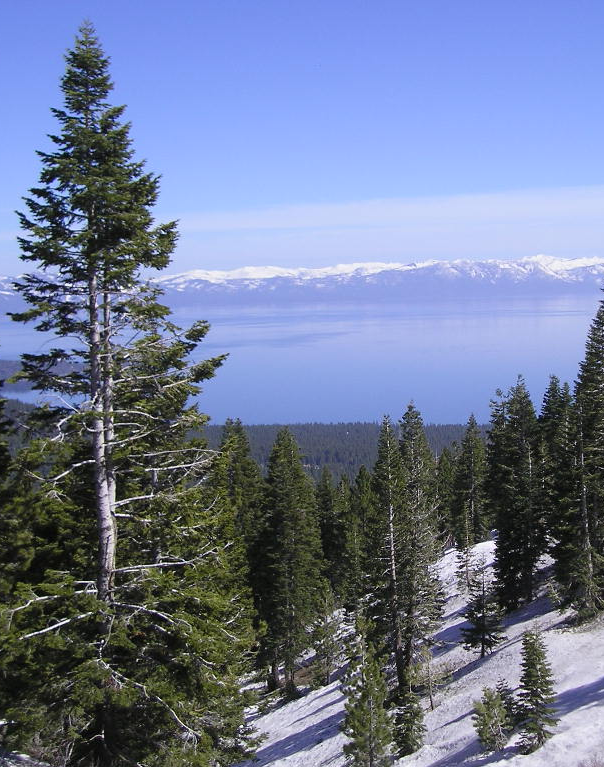
\includegraphics[width=\paperwidth,height=\paperheight]{background.jpg}
\vfill
}}}

\begin{document}

% INPUTTING BACKGROUND IMAGE
\AddToShipoutPicture{\BackgroundPic}
\vbox{}
\pagestyle{empty}
\newpage
\textwidth=15.5cm
\ClearShipoutPicture
\newpage

\section*{}

\vspace*{60mm}
ISBN ???-??-????-???-?\\ \\
This is a joint publication of the 
University of Nevada (Reno), 
Desert Research Institute (Reno),
Idaho National Laboratory (Idaho Falls),
U.S. Army R\&D Center (Vicksburg), 
Institute of Thermomechanics (Prague, Czech Republic), 
and University of West Bohemia (Pilsen, Czech Republic).\\

\noindent
FEMTEC 2011:
3rd International Conference on Computational Methods in Engineering and Science\\

\noindent
\begin{tabular}{ll}
Editors: & Pavel Solin (University of Nevada, Reno \& Institute of Thermomechanics, Prague) \\
& Glen Hansen (Idaho National Laboratory)\\
& Pavel Karban (University of West Bohemia, Pilsen) \\
& Chris Kees (U.S. Army R\&D Center, Vicksburg, Mississippi) \\
& Darko Koracin, Matt Reeves (Desert Research Institute, Reno) \\
Publisher: & University of Nevada, Reno \\
& 1664 North Virginia Street \\
& Reno, NV 89557 - 0084\\
& U.S.A.\\
Printed by: & XXXXXXXXX \\
& XXXXXXXXX\\
& XXXXXXXXX\\
Year: & 2011\\
\end{tabular}

\subsection*{Contact Information}

Mailing address:\\
FEMTEC 2011 Conference\\
Department of Mathematics and Statistics\\
University of Nevada, Reno, NV 89557 - 0084\\ 

\noindent
E-mail: {\tt femtec2011@unr.edu}\\
Web page: {\tt http://hpfem.org/events/femtec-2011/}\\
Phone: 1-775-848-7892

\chapter*{\huge FEMTEC 2011}
\vspace{-5mm}
\normalsize   
\begin{center}
3rd International Conference on Computational Methods in Engineering and Science\\
Harvey's Casino and Resort\\ 
May 9 - 13, 2011\\
\end{center}
\vspace{-3mm}

\section*{Conference topics}

\begin{itemize}
\item Computational methods in geosciences including, but not limited to, 
      atmospheric sciences (weather and climate), hydrology, geology, 
      atmospheric chemistry, air pollution, and related disciplines. 
\item Computational methods in nuclear, mechanical, civil, electrical, and 
      other engineering fields. 
\item Mesh generation and scientific visualization. 
\item Open-source scientific computing software.
\item Interactive browser tools, web-based computing and visualization.
\item Python in open source scientific computing projects.
\item Novel scientific computing tools such as SciPy, NumPy, SymPy etc.
\item Common platforms for scientific computing, interfacing and interoperability.
\end{itemize}

\subsection*{Scientific Committee}

\begin{itemize}
\item Valmor de Almeida (Oak Ridge National Laboratory, Oak Ridge, USA)
\item Ivo Dolezel (Czech Technical University, Prague, Czech Republic)
\item Glen Hansen (Idaho National Lab, Idaho Falls, USA)
\item Pavel Karban (University of West Bohemia, Pilsen, Czech Republic)
\item Christopher Kees (U.S. Army Engineer Research and Development Center, USA)
\item Matthew Knepley (University of Chicago, USA)
\item Darko Koracin (Desert Research Institute, Reno, USA)
\item Dmitri Kuzmin (University of Erlangen, Germany)
\item Stephane Lanteri (INRIA, France)
\item Matthias Moeller (Technical University of Dortmund, Germany)
\item Sascha Schnepp (Technical University of Darmstadt, Germany)
\item Stefan Turek (Technical University of Dortmund, Germany)
\item Gael Varoquaux (CEA Saclay, France)
\end{itemize}

\subsection*{Organizing Committee}

\begin{itemize}
\item Pavel Solin (University of Nevada, Reno and Institute of Thermomechanics, Prague)
\item Glen Hansen Idaho National Laboratory, Idaho Falls
\item Pavel Karban  (University of West Bohemia, Pilsen)
\item Christopher Kees U.S. Army Engineer R\& Center, Vicksburg
\item Darko Koracin, Matt Reeves, Desert Research Institute, Reno
\end{itemize}

\newpage
{\ }
\tableofcontents
\pagestyle{plain}

%--------------------------------------------------------------------------------------
%--------------------------------------------------------------------------------------

\part{Abstracts of Keynote Lectures}

\title{Finite Elements in Coastal Ocean Circulation Modeling}
\author{} \institute{}
\tocauthor{C.~Dawson}
\maketitle

\begin{center}
{\large Clint Dawson}\\
The University of Texas at Austin\\
{\tt clint@ices.utexas.edu}
\end{center}

\section*{Abstract}
Finite element methods of various types have been implemented by a number of researchers for modeling global and regional ocean circulation.  In this talk, we will discuss and compare two approaches investigated by the author and several collaborators for modeling circulation in the coastal ocean: a continuous Galerkin finite element method based on the generalized wave continuity equation (GWCE) \cite{dawson1}, and a discontinuous Galerkin (DG) formulation \cite{dawson2,dawson3} based on the primitive form of the shallow water equations.

The GWCE is the basis for the Advanced Circulation (ADCIRC) model \cite{dawson4}, which is a widely used quasi-operational shallow water simulator.    While this model has been shown to work well in many ``real-world'' situations, such as in modeling hurricane storm surges in the Gulf coast of the U.S. \cite{dawson5}, it suffers from some drawbacks, including mass conservation errors, stability isues, and is restricted to low order approximations.  The DG formulation has certain potential advantages, including local mass conservation, the use of numerical fluxes and slope-limiters to prevent spurious oscillations, and the ability to use higher-order approximations locally within an element.

We will compare both methods for standard model problems, examining both accuracy and parallel efficiency.  We will also discuss how features particular to coastal regions, such as wetting/drying and levees, are handled in each model. Finally, we will discuss results for both models  applied to actual hurricanes along the Gulf of Mexico coast, including Hurricane Ike, which hit Texas in 2008.  We will conclude with a discussion of current challenges and future research directions.

\bibliographystyle{plain}
\begin{thebibliography}{10}
\bibitem{dawson1}
\textsc{D. R. Lynch and W. R. Gray}. {A wave equation model for finite element computations}. Computers and Fluids, 7, pp.\ 207-228, 1979.  

\bibitem{dawson2}
\textsc{V.~Aizinger, C.~Dawson}. {A discontinuous Galerkin method for two-dimensional flow and transport in shallow water}. Advances in Water Resources, 25, pp.\ 67-84, 2002

\bibitem{dawson3}
\textsc{E. J.~Kubatko, J. J.~Westerink, C.~Dawson}. {$hp$ Discontinuous Galerkin methods for advection dominated problems in shallow water flow}. Comput.~Meth.~Appl.~Mech.~Engrg.~196, pp. 437--451, 2006.

\bibitem{dawson4}
\textsc{R. A. Luettich, J. J. Westerink and N. W. Scheffner}. {ADCIRC: An advanced three-dimensional circulation model for shelves, coasts and estuaries}. Report 1: Theory and methodology of ADCIRC-2DDI and ADCIRC-3DL, Dredging Research Program Technical Report DRP-92-6, U.S. Army Engineers Waterways Experiment Station, Vicksburg, MS, 1992.

\bibitem{dawson5}
\textsc{S.~Bunya, J.C.~Dietrich, J.J.~Westerink, B.A.~Ebersole, J.M.~Smith,  J.H.~Atkinson, R.~Jensen, D.T.~Resio, R.A.~Luettich, C.~Dawson, V.J.~Cardone, A.T.~Cox, M.D.~Powell, H.J.~Westerink, H.J.~Roberts}. {A high-resolution coupled riverine flow, tide, wind, wind wave and storm surge model for Southern Louisiana and Mississippi: Part I - Model development and validation}. Monthly Weather Review, 138, pp. 345--377, DOI: 10.1175/2009MWR2906.1, 2010.  

%\bibitem{dawson6}
%\textsc{J.C.~Dietrich, S.~Bunya, J.J.~Westerink, B.A.~Ebersole, J.M.~Smith,  J.H.~Atkinson, R.~Jensen, D.T.~Resio, R.A.~Luettich, C.~Dawson, V.J.~Cardone, A.T.~Cox, M.D.~Powell, H.J.~Westerink and H.J.~Roberts}. {A high-resolution coupled riverine flow, tide, wind, wind wave and storm surge model for Southern Louisiana and Mississippi: Part II - Synoptic description and analyses of Hurricanes Katrina and Rita}. Monthly Weather Review, 138, pp.\ 378--404, DOI: 10.1175/2009MWR2907.1, 2010.

%\bibitem{dawson7}
%\textsc{J.C.~Dietrich, J.J.~Westerink, A.B.~Kennedy, J.M.~Smith,R.~Jensen, M.~Zijlema, L.H.~Holthuijsen, C.~Dawson, R.A.~Luettich, Jr., M.D.~Powell, V.J.~Cardone, A.T.~Cox, G.W.~Stone, M.E.~Hope, S.~Tanaka, L.G.~Westerink, H.J.~Westerink, and Z.~Cobell, Hurricane Gustav}. {(2008) waves, storm surge and currents:  Hindcast and synoptic analysis in Southern Louisiana}. submitted to Monthly Weather Review.

%\bibitem{dawson8}
%\textsc{E.~Kubatko, S.~Bunya, C.~Dawson and J.J.~Westerink}. {Dynamic $p$-adaptive Runge-Kutta discontinuous Galerkin methods for the shallow water equations}. Comput.~Methods Appl.~Mech.~Engrg., 198, pp.\ 1766--1774, 2009.
\end{thebibliography}
\newpage


% *****************************
% *   YOUR TEXT STARTS HERE   *
% *****************************

\title{Scalability of Trilinos: People, Processes and Parallelism}
\author{} \institute{} % Intentionally left blank
\tocauthor{Michael A. Heroux}
\maketitle
\begin{center}
{\large Michael Heroux}\\
Sandia National Labs, Albuquerque, NM\\
{\tt maherou@sandia.gov}\\
\end{center}

\section*{Abstract}

Trilinos~\cite{trilinoshomepage,Trilinos-Overview-TOMS} is a large collection of open source libraries for scalable technical computing, winner of an R\&D 100 award and the HPC Software Challenge award at the IEEE/ACM Supercomputing conference in 2004.  The name Trilinos is a Greek term that loosely translates to ``a string of pearls'' and is meant to evoke the image of useful, independently-developed packages that are even more valuable as a collection.  Although the ``Tri'' in Trilinos symbolizes our grand vision of 3 packages when the project started ten years ago, we quickly realized that the community, infrastructure and package concepts were useful on a broader scope.  Presently Trilinos contains approximately 60 packages and continues growing.  

The computing community is in the early years of a fundamental shift in parallel computing from single core nodes to large-count multicore and GPU (collectively called manycore) nodes.  Trilinos is well on the path to execution on scalable manycore systems, providing basic computational capabilities using OpenMP, Pthreads, Intel Threading Building Blocks and CUDA.  Presently we are performing research and development in manycore algorithms in areas such as sparse factorizations and solves, communication-avoiding methods and multi-precision methods.

In this presentation we discuss how we are addressing scalability of Trilinos in (i) coordinating the efforts of project contributors, (ii) developing processes that enable scalability in package count and (iii) migration to new parallel systems at the desktop, department and computing center design points.

We conclude the presentation with lessons learned about large-scale scientific software engineering and our view of architecting software for current and future parallel systems.

\bibliographystyle{plain}
%\bibliography{/Users/maherou/Software/research/bibliography/mybib}
\begin{thebibliography}{1}

\bibitem{trilinoshomepage}
{Michael A. Heroux and James M. Willenbring and Roscoe A. Bartlett and Andrew
  G. Salinger and Jonathan Hu and Pavel Bochev and Karen Devine and Ron
  Oldfield}.
\newblock {Trilinos Home Page}, 2011.
\newblock http://www.trilinos.org.

\bibitem{Trilinos-Overview-TOMS}
{Michael A. Heroux and Roscoe A. Bartlett and Vicki E. Howle and Robert J.
  Hoekstra and Jonathan J. Hu and Tamara G. Kolda and Richard B. Lehoucq and
  Kevin R. Long and Roger P. Pawlowski and Eric T. Phipps and Andrew G.
  Salinger and Heidi K. Thornquist and Ray S. Tuminaro and James M. Willenbring
  and Alan Williams and Kendall S. Stanley}.
\newblock {{An Overview of the Trilinos Project}}.
\newblock {\em ACM Trans. Math. Softw.}, 31(3):397--423, 2005.

\end{thebibliography}

\newpage
\title{Solution Methods for Multiple-time-scale Multiphysics Systems: Application to Transport/Reaction and Resistive MHD}
\author{J. N. Shadid et. al.} \institute{Sandia National Laboratories}
\tocauthor{R. P. Pawlowski, E. C. Cyr, P. T. Lin, R. S. Tuminaro}

\begin{center}

\textbf{\Large Solution Methods for Multiple-time-scale Multiphysics Systems: Application to Transport/Reaction and Resistive MHD}\\
\vspace{10mm}
{\large \underline{J. N. Shadid}, R. P. Pawlowski, E. C. Cyr, P. T. Lin, R. S. Tuminaro}\\
Sandia National Laboratories\\
{\tt jnshadi@sandia.gov}\\
\vspace{4mm}
{\large L. Chacon}\\
Oak Ridge National Laboratory

\end{center}

\section*{Abstract}

A current challenge before the computational science and numerical mathematics community is the efficient computational solution of multiphysics systems.  These systems are strongly coupled, highly nonlinear and characterized by multiple physical phenomena that span a very large range of length and time scales.   These characteristics make the scalable, robust, accurate, and efficient computational solution of these systems over, relevant dynamical time scales of interest extremely challenging.

In this presentation I will discuss issues related to the stable, accurate and efficient time integration, nonlinear, and linear solution of multiphysics systems. The discussion will begin with a few illustrative examples that compare operator split and semi-implicit approaches, to fully-coupled fully-implicit methods. I will then overview a number of the important fully-coupled solution methods that our research group has applied to the solution of coupled multiple-time-scale multi-physics systems. The solution methods that we employ include, fully-implicit time integration, direct-to-steady-state solution methods, continuation, bifurcation, and optimization techniques that are based on Newton-Krylov iterative solvers [1,2]. To enable the robust, scalable and efficient solution of large-scale sparse  linear systems algebraic multilevel (AMG) preconditioners are employed. These include a fully-coupled graph-based aggregation AMG technique [3] and approximate block factorization techniques [4]. To demonstrate the capability of these methods I will present representative results for solution of transport / reaction and resistive 
magneto-hydrodynamic systems with stabilized finite element methods. In this context I will discuss robustness, efficiency, and the parallel and algorithmic scaling of the solution methods.

This work was partially supported by  the DOE office of Science AMR program at Sandia National Laboratory. Sandia is a multiprogram laboratory operated by Sandia Corporation, a Lockheed Martin Company, for the United States Department of Energy's National Nuclear Security Administration under contract DEM-AC04-94AL85000

\bibliographystyle{plain}
\begin{thebibliography}{10}

\bibitem{EwingWangYang03}
{\sc M. Sala and R.S. Tuminaro}. {Jacobian-free {N}ewton--{K}rylov methods: a survey of approaches and applications}. J. Comput. Phys 31 (2004), pp.~357--397.

\bibitem{CockburnGopalakrishnan04}
{\sc J. N. Shadid, A. G. Salinger, R. P. Pawlowski, P. T. Lin, G. L. Hennigan, R. S. Tuminaro and R. B. Lehoucq}. {Large-scale Stabilized FE Computational Analysis of Nonlinear Steady State Transport/Reaction Systems}. CMAME 195 (2006), pp.~1846--1871.

\bibitem{EwingWangYang03}
{\sc M. Sala and R.S. Tuminaro}. { A new Petrov-Galerkin smoothed aggregation preconditioner for nonsymmetric linear systems}. SIAM J. Sci. Stat. 31 (2008), pp.~143--166.

\bibitem{A104}
{\sc H. Elman, V. Howle, J. N.  Shadid, R. Shuttleworth, and R. Tuminaro}.
\newblock A Taxonomy of Parallel Mulit-level Block Preconditioners for the Incompressible Navier-Stokes Equations.
\newblock J. Comp. Phys. 227 (2008), pp. 1790 --  1808. 

\end{thebibliography}\newpage
\title{The Challenge to Provide Computational Tools for Increasingly Complex Models and Physics}
\author{} \institute{}
\tocauthor{L.~M.~Taylor}
\maketitle

\begin{center}
{\large Lee M. Taylor}\\
ANATECH Corp., San Diego, CA\\
{\tt taylor@anatech.com}
\end{center}

\section*{Abstract}
The use of computational methods in nuclear, civil and other engineering fields has become routine as the theory and algorithms have matured over the past fifty years. Nonlinear analysis including both geometric large deformations and nonlinear materials is now common. The size and complexity of the models and the necessity to perform multi-physics simulations is the big challenge for the computational mechanics community. Increasingly, the demand from the analyst community is for easy-to-use, cost-effective, time efficient analysis tools for these more complex problems. Three-dimensional analyses using the TeraGrande finite element code \cite{taylor1} will be presented to illustrate the concepts discussed in this presentation. The examples will include of aircraft impact on large pre-stressed concrete structures\cite{taylor2}, geomechanics solutions of deformations in highly faulted and stratified oil reservoirs, and blast loading on buried underground structures.

With the advent of geometry-based automatic mesh generation, engineers can now create extremely detailed finite element models that contain many parts with complex geometry. Models with millions of finite elements and hundreds of parts are now routinely generated. The ease of model generation is rapidly outpacing the ability of the computational engines to perform the analyses in a timely manner. The computational effort required for the analysis of the models is generally dominated by the CPU time spent in the equation solver and in the contact search and tracking algorithms required to determine the physical contact interactions between the parts. To reduce the turn-around time for large complex models, parallel algorithms using multiple processors are becoming common. Algorithms and the software architectures will be presented that address the issues required for successfully spanning the range from a handful of processors up to the massively parallel case of thousands of
processors in the context of both shared memory and distributed memory hardware.

%The complexity of the models is also driven by an increasing use of highly nonlinear material models that include material failure and deletion. It is no longer sufficient to simply predict the nonlinear stresses and strains in the model. Now the analyst wants to predict tearing or perforation of the parts of the model. The contact search and tracking algorithms must now determine contact between parts that have eroding surfaces. This is complicated by the requirement that these algorithms perform in a multi-processor parallel analysis. Contact algorithms will be presented that address these issues.

Geometry-based model generation using automatic mesh generation is dominated by tetrahedral finite element meshes. Tetrahedral meshes inherently have element counts much larger than comparable hexahedral meshes and exacerbate the problems of mesh size. Furthermore, mesh quality is always an issue. Some examples of tetrahedral models in the context of these issues will be presented.

\bibliographystyle{plain}
\begin{thebibliography}{1}
\bibitem{taylor1} 
\textsc{ANATECH Corp.}.
\newblock{TeraGrande User's Manual -- Version 1.0}.
\newblock{San Diego, CA, 2005.}

\bibitem{taylor2}
\textsc{Y. R. Rashid, R. J. James, et.al.}
\newblock{{Failure Analysis and Risk Evaluation of Lifeline Structures Subjected to Blast Loadings and Aircraft/Missile Impact,}}
\newblock{Proceedings of the International Workshop on Structures Response to Impact and Blast, Technion, Israel Institute of Technology, Haifa, Israel, November 15--17, 2009.}
\end{thebibliography}
\newpage
\title{GPU-Accelerated Computing}
\author{} \institute{}
\tocauthor{\underline{S.~Kodiyalam}, S.~Posey, H.~Lee}
\maketitle

\begin{center}
{\large \underline{Srinivas Kodiyalam}, Stan Posey, Hyung Lee}\\
NVIDIA Corporation\\
{\tt skodiyalam@nvidia.com, sposey@nvidia.com, hblee7060@gmail.com}
\end{center}

\section*{Abstract}
Current trends in high performance computing (HPC) are moving towards the availability of several cores on the same chip of contemporary processors in order to achieve speed-up through the extraction of potential fine-grain parallelism of applications. The trend is led by GPUs, which have been developed exclusively for computational tasks as massively-parallel co-processors to the CPU. During 2010 an extensive set of new HPC architectural feature were developed in the third generation of NVIDIA GPUs (Fermi), giving computational mechanics an opportunity to expand use of GPU modelling and simulation.

This presentation will examine examples relevant to industry-scale HPC practice of GPU-accelerated computational structural mechanics and computational fluid dynamics software that support product design in manufacturing industries. For each example, the choice of CPU-GPU system configurations will be described based upon the physics features, and resolution requirements of a particular simulation. Performance results compare use of conventional CPUs with and without GPU acceleration.

\bibliographystyle{plain}
\begin{thebibliography}{10}
\bibitem{kodiyalam1}
\textsc{R. Lucas, G. Wagenbreth, D. Davis}. {Implementing a GPU-Enhanced Cluster for Large Scale Simulations}. I/ITSEC, 2007. Orlando, FL.  

\bibitem{kodiyalam2}
\textsc{S. Kodiyalam, M. Kremenetsky, S. Posey}. {Balanced HPC Infrastructure for CFD and Associated Multidiscipline Simulations of Engineering Systems}. 7th Asia CFD Conference 2007. Bangalore, India, November 26 – 30, 2007.

\bibitem{kodiyalam3}
\textsc{A. Corrigan, F. Camelli, R. Lohner, Mut, F.}. {Porting of an edge-based CFD solver to GPUs}. 48th AIAA Aerospace Sciences Meeting Including The New Horizons Forum and Aerospace Exposition, number AIAA-2010-522. Orlando, FL, January 2010.

\bibitem{kodiyalam4}
\textsc{P. LeGresley, E. Elsen, E. Darve}. {Large calculation of the flow over a hypersonic vehicle using a GPU}. Journal of Computational Physics, 227:10148-10161. 2008.

\bibitem{kodiyalam5}
\textsc{N. Bell, M. Garland}. {Implementing sparse matrix-vector multiplication on throughput-oriented processors}. SC '09: Proceedings of the Conference on High Performance Computing Networking, Storage and Analysis, pages 1-11. New York, NY, USA, 2009. ACM.

\bibitem{kodiyalam6}
\textsc{T. Brandvik, G. Pullan}. {An accelerated 3D Navier-Stokes Solver for Flows in Turbomachines}. Proceedings of GT2009 ASME Turbo Expo 2009: Power for Land, Sea and Air, June 2009.

\bibitem{kodiyalam6}
\textsc{ACUSIM Corporation, AcuSolve}. www.acusim.com.
\end{thebibliography}\newpage

%--------------------------------------------------------------------------------------

\part{Abstracts of Contributed Lectures}

\title{Anisotropic Thermal Conductivity of Cermet Nuclear Waste}
\author{} \institute{}
\tocauthor{\underline{V.~F.~de~Almeida}, C.~Ausmus, R.~T.~Jubin, P.~Solin}
\maketitle

\begin{center}
{\large \underline{Valmor F. de Almeida}, Clint Ausmus, and Robert T. Jubin}\\
Oak Ridge National Laboratory\\
{\tt dealmeidav@ornl.gov}\\
\vspace{4mm}

{\large Pavel Solin}\\
University of Nevada\\
{\tt solin@unr.edu}
\end{center}

\section*{Abstract}
Cermet is a microscopically heterogeneous material by design wherein a  ceramic phase coexists with a metal phase. One of the objectives of this combination is to improve heat removal from the  ceramic phase in this nuclear waste form. The purpose of this work is to develop methods to predict effective thermal conductivity coefficients from knowledge of the microstructure of the material. This transport property is required in coarser continuum models for thermo-mechanics of cermet material bodies. This work describes the use of hp-adaptivity using HERMES-2D in two disparate applications that share the same mathematical framework. In one application, a heat-conduction-like equation is used in the image processing of cermet elemental maps obtained with scanning electron microscopy (SEM) to identify solid phases. In the other application, a corresponding multi-phase, micro-continuum heat conduction equation is solved to obtain the temperature field which provides the means for deriving an averaged thermal conductivity tensor. Results show that a cylindrical pellet of cermet nuclear waste  may experience higher heat flux in the radial direction by as much as 30\% when compared to the axial direction. In addition, results suggest that the material is nearly orthotropic and they demonstrate that simple volume fraction average overestimates heat conduction.

\begin{figure}
\centering
\begin{tabular}{cccc}
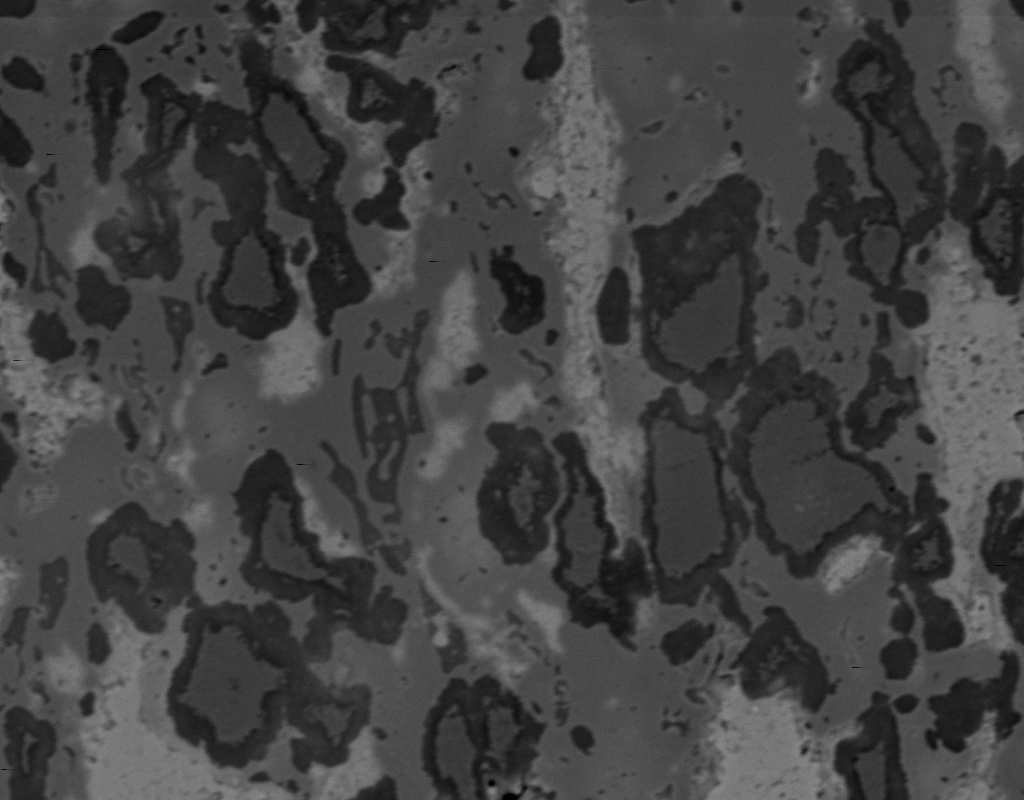
\includegraphics[height=1.1in]{./almeida/cermet-SEM.png} &
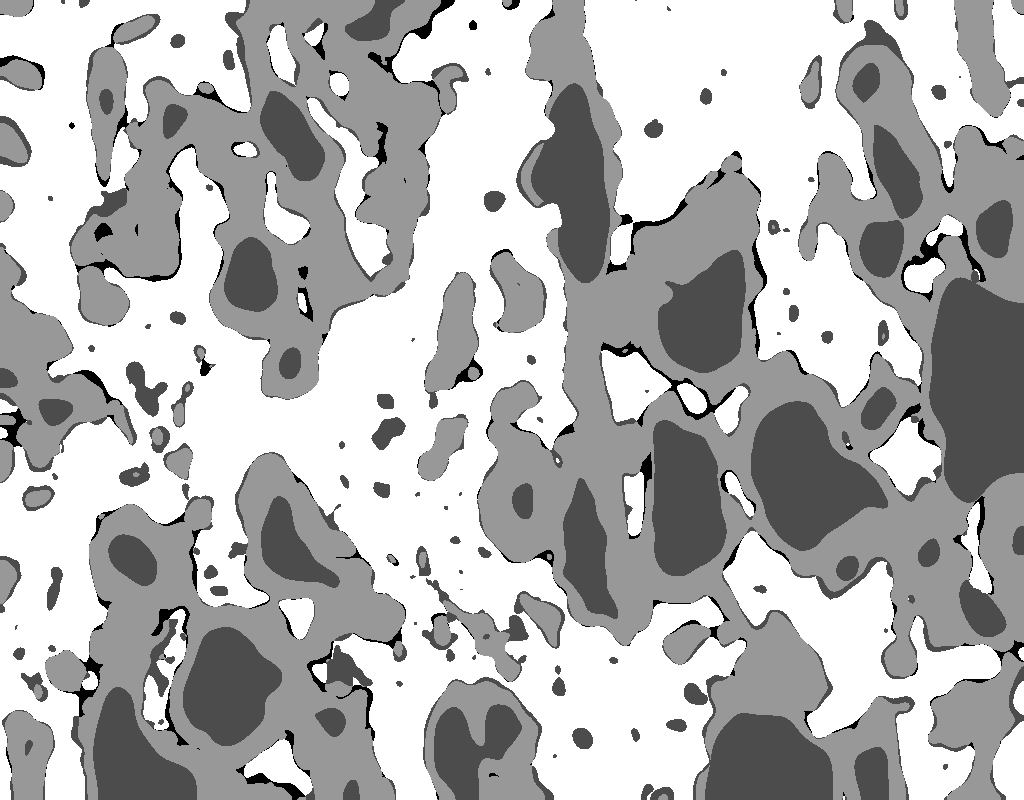
\includegraphics[height=1.1in]{./almeida/cermet-phases.png} &
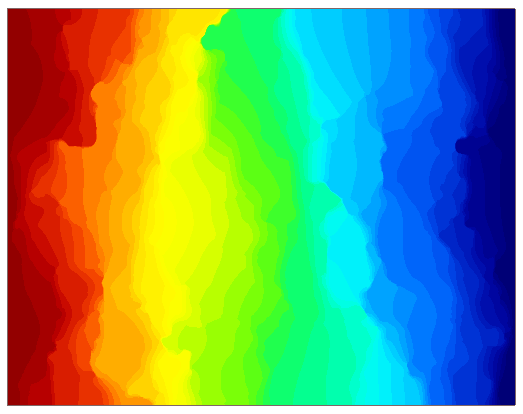
\includegraphics[height=1.1in]{./almeida/cermet-xtfield.png} &
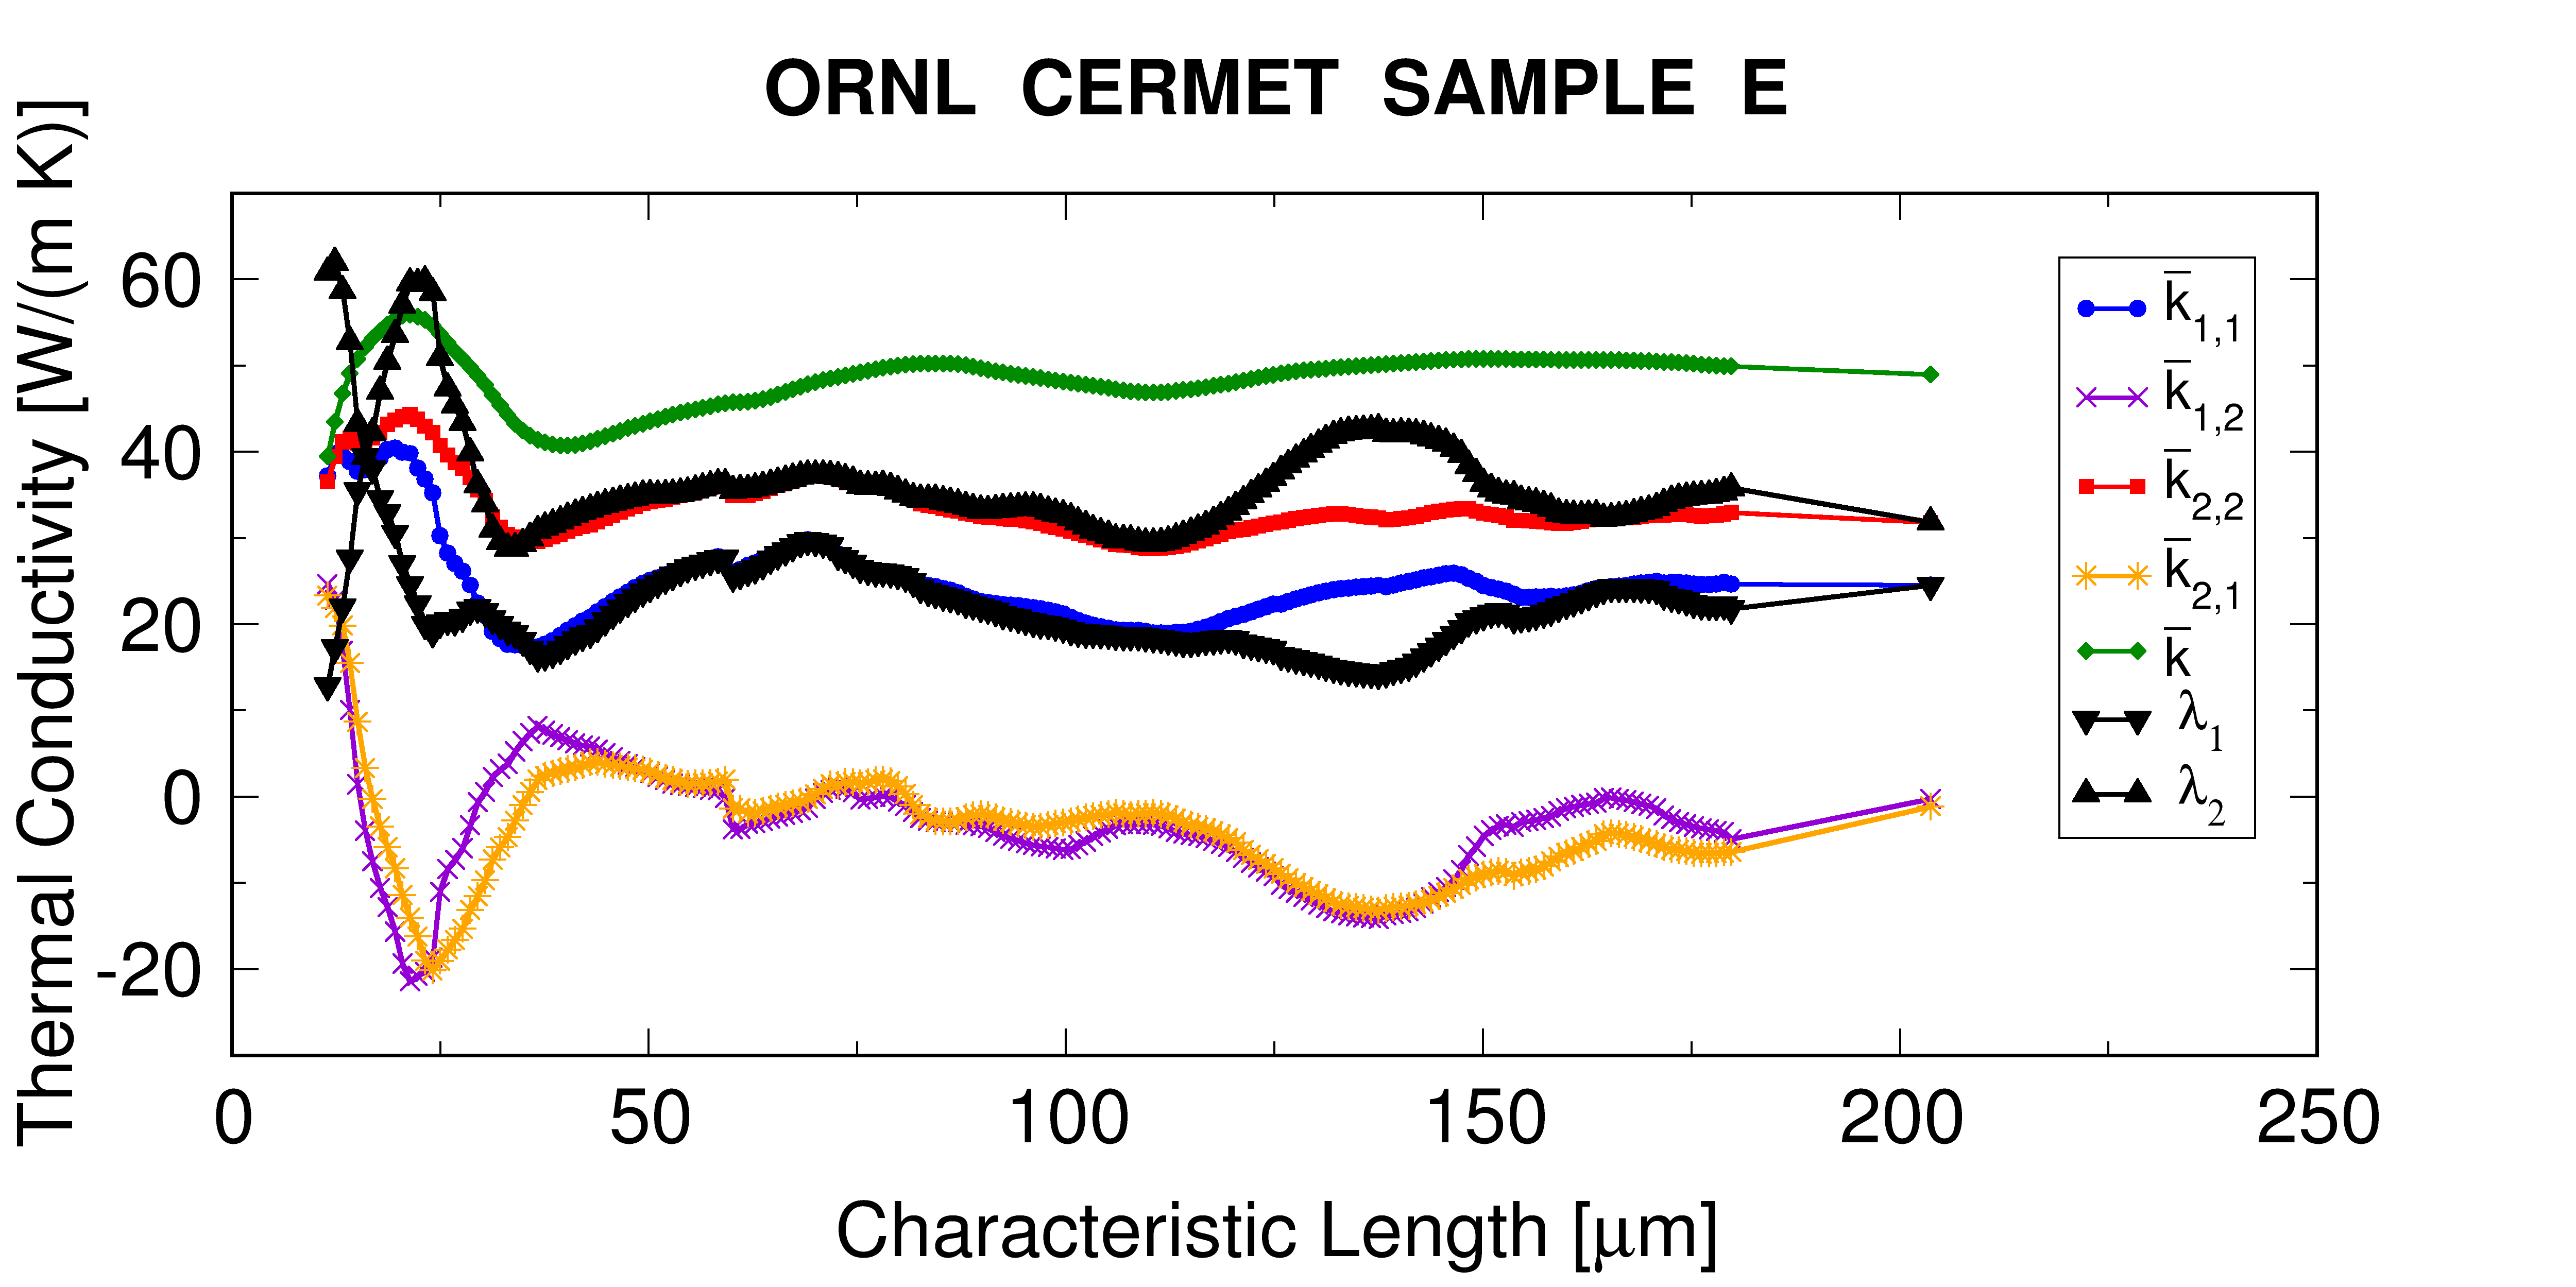
\includegraphics[height=1.1in]{./almeida/cermet-ktensor.png}
\\
(a) & (b) & (c) & (d)
\end{tabular}

\caption[Anisotropic thermal conductivity of cermet nuclear waste]{Main steps for computing the effective thermal conductivity tensor of a cermet waste form. \textbf{(a)} SEM image at origin of $z$--$r$ plane of pellet (${230x180\mathrm{\mu}m}^{2}$). \textbf{(b)} Multiphase segmentation using non-linear, inhomogeneous, anisotropic diffusion. \textbf{(c)} Temperature field when the sample is heated horizontally (a similar realization is applied vertically). \textbf{(d)} Averaging length scale variation of the derived thermal conductivity tensor components $\kappa_{i,j}$, eigenvalues $\lambda_i$, and volume fraction average conductivity $\overline{\kappa}$.}
\end{figure}

\bibliographystyle{plain}
\begin{thebibliography}{10}
\bibitem{jubin-etal-11}
{\sc R.T.~Jubin \emph{et al.}}. {Development of advanced cermet waste forms}. Waste Management Conference 2011, February 27--March 3, Phoenix, AZ.
\end{thebibliography}\newpage % Prilis dlouhe
\title{Geometrically Nonlinear Bending and Buckling Analysis of Shallow Spherical Shells}
\author{} \institute{}
\tocauthor{\underline{M.~Altekin}, R.~F.~Yukseler}
\maketitle

\begin{center}
{\large \underline{M. Altekin}, R. F. Yukseler}\\
Department of Civil Engineering, Yildiz Technical University\\
{\tt altekin@yildiz.edu.tr, yukseler@yildiz.edu.tr}
\end{center}

\section*{Abstract}
Geometrically nonlinear analysis of shallow spherical shells under uniform external pressure is made. Ordinary differential nonlinear shell equations are solved numerically by the finite difference and the Newton-Raphson methods. Totally six unkowns (three displacements and three stress resultants) are considered at each point along the radial coordinate. The study includes two cases: (i) the bending analysis is made by computing the displacements and stress resultants for uniform pressure, and (ii) the deflection-load curve is traced and the value of the external load corresponding to the first extremum of this curve is regarded as the critical (buckling) load. The material is assumed to be isotropic and homogeneous. The influence of the parameter of depth on the deflection and the critical load is investigated. The results obtained in the current work are compared with those available in the open literature.

\bibliographystyle{plain}
\begin{thebibliography}{10}
\bibitem{YamadaUchiyamaYamada83}
{\sc S.~Yamada, K.~Uchiyama, and  M.~Yamada}. {Experimental investigation of the buckling of shallow spherical shells}. Int. J. of Nonlinear  Mechanics 18  (1983), pp.~37--54.

\bibitem{TengRotter89}
{\sc J.G.~Teng, and J.M.~Rotter}. {Elastic-plastic large deflection analysis of axisymmetric shells}. Computers and Structures 31 (1989), pp.~211--233.

\bibitem{Huang64}
{\sc N.C.~Huang}. {Unsymmetrical buckling of thin shallow spherical shells}. J. of Applied Mechanics. 1 (1964), pp.~447--457.

\bibitem{Uddin87}
{\sc M.D.W. ~Uddin}. {Buckling of general spherical shells under external pressure}. Int. J. of Mechanical Sciences.  29 (1987), pp.~469--481.

\bibitem{Kai-YuanWei-PingCleghorn94}
{\sc Y.~Kai-Yuan, S.~Wei-Ping, and W.L.~Cleghorn}. {Axisymmetric buckling of thin shallow circular spherical shells under uniform pressure for large values of geometric parameter}. Int. J. of Nonlinear Mechanics 29 (1994), pp.~603--611.

\bibitem{NowinkaLukasiewicz91}
{\sc J.~Nowinka, and S.~Lukasiewicz}. {Symmetric elements in geometrical analysis of large deformations of spherical shells}. Int. J. of Nonlinear Mechanics. 26 (1991), pp.~151--168.
\end{thebibliography}\newpage
\title{An Efficient Preconditioner for Elliptic Problems Discretized by High-Order Finite Element Problems}
\author{} \institute{}
\tocauthor{\underline{T.~Austin}, B.~Jamroz, C.~Jhurani, M.~Brezina, T.~Manteuffel, J.~Ruge}
\maketitle

\begin{center}
{\large \underline{Travis Austin}, Ben Jamroz, Chetan Jhurani}\\
Tech-X Corporation\\
{\tt austin@txcorp.com}\\
\vspace{4mm}

{\large Marian Brezina, Thomas Manteuffel, John Ruge}\\
Department of Applied Mathematics, University of Colorado
\end{center}

\section*{Abstract}
The popularity of the high-order finite element method has grown with the increased awareness that greater accuracy can be achieved for a given amount of computational work compared against the linear finite element method.  However, for a given mesh size, the higher-order finite element method yields less sparse matrices that can have an impact on iterative solver performance.   Direct usage of preconditioned Krylov methods designed for linear finite element problems may not achieve the best possible linear solver performance over one carefully tailored to the problem at hand.

For example, the wider stencil patterns found in high-order finite element matrices increases the memory consumed by the algebraic multigrid method (AMG) at all levels.  To reduce the memory and yield a more efficient preconditioner, researchers have proposed a preconditioner built from a low-order version of the high-order finite element matrix \cite{Ors1980,Heys2005}. In \cite{Heys2005}, it was established that for polynomial order $p > 4$, this sparser preconditioner is more efficient for 2D Poisson's equation than preconditioning the original high-order finite element system with algebraic multigrid built from the higher-order system.  

The approach of \cite{Ors1980,Heys2005} requires rediscretizing the problem on a finer finite element mesh constructed from the nodes of the high-order finite elements.  We have designed a method that automatically constructs a lower-order matrix by constructing sparse versions of dense, high-order element stiffness matrices and then employing these sparser element stiffness matrices in a global assembly routine \cite{Aus2011}.  The sparseness pattern can be constructed automatically and the sparse matrix entries can be calculated using a small least-squares problem.  We present recent results using this method for elliptic problems, and compare to the canonical two-level additive Schwarz method \cite{Fis1997}.  We consider uniform and non-uniform meshes and techniques for reducing the cost of the sparse preconditioner setup.  Results are presented for the single processor case as well as for hundreds of processors.

\bibliographystyle{plain}
\begin{thebibliography}{10}
\bibitem{Ors1980}
\textsc{S.~Orszag}. {Spectral methods for problems in complex geometries}. J. Comp. Phys. 37 (1980), pp.~70--92.

\bibitem{Heys2005}
\textsc{J.~Heys, T.~Manteuffel, S.~McCormick, L.~Olson}. {Algebraic multigrid for higher-order finite elements}. J. Comp. Phys. 204 (2005),  pp.~520--532.

\bibitem{Aus2011}
\textsc{T.~Austin, M.~Brezina, T.~Manteuffel, J.~Ruge}. {Automatic construction of sparse preconditioners for high-order finite element problems.} Accepted for publication in Bentham eBook: {\em Efficient Preconditioned Solution Methods for Elliptic Partial Differential Equations}. 

\bibitem{Fis1997}
\textsc{P.~Fischer}. {An overlapping Schwarz method for spectral element solution of the incompressible Navier-Stokes equations.} J. Comp. Phys. 133  (1997), pp.~84--101.
\end{thebibliography}\newpage
\title{Generation of Structured Mesh in 2D Domain with Singularities on Boundary by using Elliptic PDEs}
\author{Boris Azarenok} \institute{Dorodnicyn Computing Center of Russian Academy of Sciences, Moscow}

\begin{center}

\textbf{\Large Generation of Structured Mesh in 2D Domain with Singularities on Boundary by using Elliptic PDEs}\\
\vspace{10mm}
{\large Boris Azarenok}\\
Dorodnicyn Computing Center of Russian Academy of Sciences \\ Vavilov str. 40 , Moscow, 119333, Russia \\
{\tt azarenok@ccas.ru}

\end{center}

\section*{Abstract}

In structured grid generation methods a widespread way is the use of a mapping $\mathbf F$ of the parametric domain $\mathcal P$ (square or rectangle), divided into square cells, onto the underlying physical domain $\Omega$. If the mapping $\mathbf F\,{:}\,\mathcal P{\rightarrow}\Omega$ is a homeomorphism then the image of the square mesh on the domain $\mathcal P$ is an unfolded grid on the domain $\Omega$. In a variational approach, the functions $\mathbf F{=}(f_1,f_2)$ are extremals of a functional or solution of the boundary value problem for the corresponding Euler equations. For the elliptic partial differential equations (PDEs) of the second order, to be more precise for the Laplace equations, the Rad\'o theorem \cite{Rado26} asserts that the harmonic mapping of a simply connected bounded domain onto a simply connected bounded convex domain is univalent subject to a given homeomorphism between their boundaries. To satisfy the conditions of the Rad\'o theorem on nonconvex physical domains, the inverted Laplace equations are applied (cf. \cite{Winslow67,Thomp74}). Despite the inverse harmonic mapping is a homeomorphism, its discrete realization (Winslow's method) produces a folded mesh on the domain $\Omega$ with breaks (sharp interior corners) on the boundary $\partial\Omega$. To understand the reason of grid folding we construct an analytical harmonic mapping $\mathbf F$ of the backstep domain $\Omega$ onto the parametric square $\mathcal P$. The mapping $\mathbf F\,{:}\,\Omega{\rightarrow}\mathcal P$ is sought using the conformal mapping of the unit disk onto the backstep (hexagon). This conformal mapping is sequentially performed, first, using the linear fractional map of the unit disk onto the upper half-plane and, second, Schwarz-Christoffel mapping of the upper half-plane onto the hexagon. In the unit disk, it is solved the Dirichlet problem for the each component of the harmonic mapping $f_1$ and $f_2$ by the Poisson integral. The inverse harmonic mapping $\mathbf F^{-1}{:}\,\mathcal P{\rightarrow}\Omega$ is sought by inverting numerically the analytic functions $f_1,f_2$. The obtained inverse harmonic mapping $\mathbf F^{-1}$ is very precise and close to the analytical mapping. Our solution demonstrates that the internal corner point on the backstep boundary is a singularity point where the level-set of different families are stuck, i.e. the angle between level-set $\xi{=}const$ and  $\eta{=}const$ is equal to zero. This causes the grid lines to overlap. The effect of stuck level-set at a singular point on the domain boundary is observed for the mapping produced by elliptic second-order PDEs. To eliminate mesh folding near the singular point we apply an additional local mapping. To construct the quasiconformal mapping, producing the mesh, it is solved the Dirichlet problem for quasilinear elliptic PDEs \cite{Azar09,Azar10}.


\bibliographystyle{plain}
\begin{thebibliography}{10}

\bibitem{Rado26} {\sc T.\,Rad\'o}. {Aufgabe 41}. Jahresber. Deutsche Math.-Verein. 35 (1926), p. 49.

\bibitem{Winslow67} {\sc A.M.\,Winslow}. {Numerical solution of the quasi-linear Poisson equation in a nonuniform triangle mesh}. J. Comput. Phys. 2 (1967), pp. 149--172.

\bibitem{Thomp74} {\sc J.F.\,Thompson, C.W.\,Mastin, F.C.\,Thames}. {Automatic numerical generation of body-fitted curvilinear coordinate system for field containing any
number of arbitrary two-dimensional bodies}. J. Comp. Phys. 15 (1974), pp. 299--319.

\bibitem{Azar09} {\sc B.N.\,Azarenok}. {Generation of structured difference grids in two-dimensional nonconvex domains using mappings}. Comput. Math. Math. Phys. 49 N. 5 (2009),
pp. 797--809.

\bibitem{Azar10} {\sc B.N.\,Azarenok}. {On 2D structured mesh generation by using mappings}. Numerical Methods for Partial Differential Equations. (2010), Published online in Wiley
InterScience (www.interscience.wiley.com). DOI 10.1002/num.20570.

\end{thebibliography}\newpage % Prilis dlouhe
\title{Modeling the Influence of Wind Characteristics and the Atmospheric Parameters on the Wind Turbine Performances}
\author{} \institute{}
\tocauthor{\underline{R.~Belu}, D.~Koracin}
\maketitle

\begin{center}
{\large \underline{Radian Belu}}\\
Drexel University\\
{\tt rbelu@dri.edu}\\
\vspace{4mm}

{\large Darko Koracin}\\
Desert Research Institute\\
{\tt darko@dri.edu}
\end{center}

\section*{Abstract}
The power output uncertainty is closely related to the uncertainty of the wind velocity and other meteorological parameters and their effects on wind turbine performances. For example, there is an inherent uncertainty in the power curve estimate by using the wind speed measured at the hub height. The assumption behind this is that these wind speeds are representative of the wind over the whole rotor area.  While this assumption was adequate for smaller wind turbines this is essentially not true for modern multi-MW ones, and considerable deviations often occur between the expected and produced power. Wind shear and direction, turbulence, and atmospheric stability vary with height as a result of either meteorological and/or terrain conditions. This calls for an adoption of new measurement and power estimation methods (Sumner and Masson, 2006, Wagner et al., 2007). The rotor size combined with the hub height implies that wind turbines are often exposed to highly varying wind conditions with large wind shears, turbulence and atmospheric stability variations within the rotor span. These may affect both the production and the structural safety of the turbine. Consequently, a better power or load prediction requires more representative wind measurements and power computations over the turbine's rotor. The impact of atmospheric stability, turbulence, wind shear and wind gust on the wind turbine output power and site evaluation are reviewed. Velocity, temperature, and turbulence intensity profiles are generated using Monin-Obukov similarity theory. The resulting system of nonlinear equations was solved numerically and tested against field observations. The experimental data used in this study were collected during 14 months on an 80 m instrumented meteorological tower at four levels (10 m, 40 m, 60 m, and 80 m), using sonic anemometer. The rotor's averaged wind and meteorological parameters are then evaluated by integrating the resulting velocity profile over the swept area of the rotor. Further analyses were conducted to determine if other factors accompanying the change in turbulence level and atmospheric stability could cause or contribute to the observed sensitivity of the power curves to the turbulence and atmospheric stability as reported in the literature.

\bibliographystyle{plain}
\begin{thebibliography}{10}
\bibitem{belu_11}
{\sc J.~Sumner and C. ~Masson}. {Influence of Atmospheric Stability on Wind Turbine Power Performance Curves}. J. Sol. Energy Eng. 128(2006), pp.~531--537.

\bibitem{belu_12}
{\sc R. ~Wagner, I. ~Antoniou, S.M. ~Pedersen, M.S. ~Courtney, and H.E. ~Jorgensen}. The influence of the wind speed profile on wind turbine performance measurements. Wind Energy 12(4) (2009), pp. 348--362.
\end{thebibliography}\newpage
\title{Numerical Simulation Studies for Vertical Axis Wind Turbine Performance Prediction with Applications in Built Environment}
\author{} \institute{}
\tocauthor{\underline{R.~Belu}, A.~Trzynadlowski}
\maketitle

\begin{center}
{\large \underline{Radian Belu}}\\
Drexel University\\
{\tt rbelu@dri.edu}\\
\vspace{4mm}

{\large Andrzej Trzynadlowski}\\
University of Nevada\\
{\tt chin@engr.unr.edu}
\end{center}

\section*{Abstract}
Worldwide interest in renewable energy systems has increased dramatically due to environmental concerns like climate change as well as the likely future shortages in the energy supply. Wind power is a major source of sustainable energy and can be harvested using both horizontal and vertical axis wind turbines. This paper presents studies of various configurations of vertical axis wind turbines performance for built environment. Numerical simulations are presented to predict fluid flows through the various Darrrieus wind turbine configurations. Simulations of air flows through the turbine rotor were performed to analyze the performance characteristics of the devices (Agren et al. 2005). In the last four decades several aerodynamic prediction models have been formulated for wind turbine performances and characteristics. We can identified two families pf models: stream-tube and vortex (Paraschivoiu, 1988). The former needs much less computation at the expense of accuracy. The later requires more computational resources but is more accurate. This paper presents a simplified numerical technique for simulating vertical axis wind turbine flow based on the lifting line theory and a free vortex wake model including dynamic stall effects for predicting the performances of a 3-D vertical axis wind turbine. A vortex model is used in which the wake is composed of trailing stream-wise and shedding span-wise vortices whose strengths are equal to the change in the bound vortex strength as required by the Helmholz and Kelvin theorems. Using limited computer resources the stream-tube performance prediction model is capable of predicting the overall rotor power output and the distribution of aerodynamic forces along the rotor blades. Predictions by using our method are shown to compare favorably with existing experimental data and the outputs of other numerical models. The results of the numerical simulations are used in the design and optimization of wind turbines for built environment applications.     

\bibliographystyle{plain}
\begin{thebibliography}{10}
\bibitem{Paraschivoiu88}
{\sc I.~Paraschivoiu}. {Double-Multiple Streamtube Model for Studying Vertical-Axis Wind Turbines}. AIAA Journal of Propulsion and Power, 4 (1988), pp.~370--378.

\bibitem{A104}
{\sc Agren ~O. Berg O., and M. Leijon}. {A time-dependent potential flow theory for the aerodynamics of vertical axis wind turbines}. J.~Appl. Phys. 97 (2005), pp. 1--13.
\end{thebibliography}\newpage


% *****************************
% *   YOUR TEXT STARTS HERE   *
% *****************************

\title{Uintah - an Adaptive Scalable Framework for Fluid Structure Interaction.}
\author{} \institute{} % Intentionally left blank
\tocauthor{\underline{Martin Berzins},{Justin Luitjens}{Qingyu Meng}{Todd Harman}{Charles A. Wight}{Joseph R. Peterson} }
\maketitle
\begin{center}
\vspace{-4mm} % Use this space when including 3rd author
{\underline {Martin Berzins}, {Justin Luitjens}, {Qingyu Meng}}\\
SCI Institute, University of Utah, Salt Lake City UT 84112\\
{\tt mb@cs.utah.edu, luitjens@cs.utah.edu,  qymeng@cs.utah.edu}
%\vspace{4mm} % Use this space when including 3rd author
%{\large \underline{Justin Luitjens}}}\\
%SCI Institute, University of Utah, Salt Lake City UT 84112\\
%{\tt luitjens@cs.utah.edu}
%\vspace{4mm} % Use this space when including 3rd author
%{\large \underline{Qingyu Meng}}}\\
%SCI Institute, University of Utah, Salt Lake City UT 84112\\
%{\tt qymeng@cs.utah.edu}

%\vspace{-4mm} % Use this space when including 3rd author
{\large {Todd Harman}}\\
Department of Mechanical Engineering, University of Utah, Salt Lake City UT 84112\\
{\tt T.Harman@utah.edu}

%\vspace{-4mm} % Use this space when including 3rd author
{\large { Charles A. Wight, Joseph R. Peterson}}\\
Department of Chemistry, University of Utah, Salt Lake City UT 84112\\
{\tt Chuck.Wight@utah.edu, Joseph.R.Peterson@utah.edu}
\vspace{-4mm} % Use this space when including 3rd author
%{\large \underline{Joseph R. Peterson}}}\\
%Department of Chemistry, University of Utah, Salt Lake City UT 84112\\
%{\tt Joseph.R.Peterson@utah.edu}
\end{center}

\section*{Abstract}
%
%Enter your abstract here. Authors of contributed lectures: Please do not 
%exceed one page including references. References to related or 
%competitive work are mandatory. Presenting author should be underlined. 
%Please do not alter the internal structure of the template. Do not 
%introduce any new definitions or commands, they cause problems during the 
%compilation of the final Book of Abstract. The Book of Abstracts will be 
%compiled using pdflatex. If using images, please make sure thay are
%in PDF or PNG. Thank you!

The Uintah Software has been developed over the last decade 
\cite{csafe2,csafe3} to 
solve fluid-structure interaction problems on structured
adaptive grids on large-scale, long-running, data-intensive
problems, \cite{fourthmit}. Uintah uses flow solvers linked to
a particle method utlizing a finite element type formulation.
The challenge of making Uintah scale to large numbers of cores
on realistic engineering applications is addressed in this presentation.
Uintah uses a particularly simple block-structured AMR method, \cite{IPDPS10}. The scalability
of this method is contrasted with the Berger-Rigoutsos approach \cite{BergerRigoutsos}. 
Uintah uses a novel asynchronous task-based approach with
fully automated load balancing. This involves out of order execution of tasks \cite{Meng}  and measurement-based
load balancing. The application of Uintah to a petascale problem
in hazard analysis arising from {\it sympathetic} explosions in which the
collective interactions of a large ensemble of explosives results in
dramatically increased explosion violence, is considered, \cite{Ber2010b}. 
The advances in scalability and combustion
modeling needed to begin to solve this problem are discussed and illustrated by prototypical
computational results. Finally the challenges of multicore
architectures, are considered as is the potential for  
high-order methods (e.g. Discontinuous Galerkin) to compute solutions with the least 
energy use per significant digit of accuracy. 

\bibliographystyle{plain}
\begin{thebibliography}{10}

\bibitem{BergerRigoutsos}
M.~Berger and I.~Rigoutsos.
\newblock An algorithm for point clustering and grid generation.
\newblock {\em IEEE Trans. Systems Man Cybernet.}, 21(5):1278--1286, 1991.

\bibitem{Ber2010b}
M.~Berzins, J.~Luitjens, Q.~Meng, T.~Harman, C.~Wight, and J.~Peterson.
\newblock Uintah - a scalable framework for hazard analysis.
\newblock In {\em Proceedings of the Teragrid 2010 Conference}, number~3, page
  (published online), 2010.

\bibitem{csafe2}
J.~D. de~St.~Germain, J.~McCorquodale, S.~G. Parker, and C.~R. Johnson.
\newblock {U}intah: {A} massively parallel problem solving environment.
\newblock In {\em Ninth {IEEE} International Symposium on High Performance and
  Distributed Computing}, pages 33--41. {IEEE}, Piscataway, NJ, November 2000.

\bibitem{fourthmit}
J.~E. Guilkey, T.~B. Harman, and B.~Banerjee.
\newblock An eulerian-lagrangian approach for simulating explosions of
  energetic devices.
\newblock {\em Computers and Structures}, 85:660--674, 2007.
 
\bibitem{IPDPS10}
J.~Luitjens and M.~Berzins.
\newblock Improving the performance of {U}intah: {A} large-scale adaptive
  meshing computational framework.
\newblock In {\em Proceedings of the 24th IEEE International Parallel and
  Distributed Processing Symposium (IPDPS10)}, 2010. 

\bibitem{Meng}
Q. Meng, J. Luitjens, M. Berzins. 
\newblock Dynamic Task Scheduling for the Uintah Framework, 
\newblock In {\em Proceedings of the 3rd IEEE Workshop on Many-Task Computing on Grids and Supercomputers (MTAGS10)}, 2010.

\bibitem{csafe3}
S.~G. Parker, J.~Guilkey, and T.~Harman.
\newblock A component-based parallel infrastructure for the simulation of
  fluid-structure interaction.
\newblock {\em Engineering with Computers}, 22:277--292, 2006.

\end{thebibliography}

% ***************************
% *   YOUR TEXT ENDS HERE   *
% ***************************
\newpage % Prilis dlouhe
\title{Simulation of Fluid Flow Through an Abrasive Water Jet Nozzle using Computational Fluid Dynamics}
\author{} \institute{}
\tocauthor{A.~Bhaskar}
\maketitle

\begin{center}
{\large Abhinav Bhaskar}\\
{\tt abhinavbhaskar@gmail.com}
\end{center}

\section*{Abstract}
The present work is a compilation of efforts to gain a fundamental knowledge of the ultra-high velocity dynamic characteristics such as the velocity distribution, pressure distribution, turbulence intensity and kinetic energy of an abrasive water jet(AWJ) system. This knowledge can help enhance the AWJ technology, understanding the kerfs formation or cutting process and modelling the various cutting performance measures that are required for process control and optimization. For this purpose, Computational fluid analysis is found to be a viable approach because direct measurements of particle velocities and visualizations of particle trajectories are very difficult for the ultrahigh speed and small dimensions involved.

The development of a theoretical approach to the evaluation of turbulent flow and particle dynamic properties in the nozzle is attractive because of difficulties associated with direct measurements in nozzles of high flow speed and small dimensions. Axis symmetric simulations have been performed with the help of commercial code (Fluent 6.3), using the standard k-e turbulence model. One way coupling was considered in the simulations, which means that the effect of the presence of the dispersed solid phase in the liquid phase was not considered. The single phase coupling is considered to avoid the calculation of frictional and viscous losses in the flow, as these factors are dependent on the shape factor and sphericity of the abrasi ve particle to be used. The inside profile of the abrasive water jet nozzle was modelled by measuring the co-ordinates of the nozzle using a co-ordinate measuring machine and feeding the co-ordinates into Gambit. The profile was meshed and analysed using commercial CFD code (6.3) The results have been compared with available experimental and theoretical results published by other investigators. These results will assist in the optimal design of premixed abrasive water-jet nozzle systems and the prediction of water jet cutting performance. The turbulence characteristics can be used by the manufacturing industries for the calculation of an optimum cutting speed.\newpage

% *****************************
% *   YOUR TEXT STARTS HERE   *
% *****************************

\title{Heat Transport Simulation for CO$_2$ Enhanced Gas Recovery}
\author{} \institute{} % Intentionally left blank
\tocauthor{\underline{Norbert B\"ottcher}, Rudolf Liedl}
\maketitle
\begin{center}
{\large \underline{Norbert B\"ottcher}, Rudolf Liedl}\\
Technische Universit\"at Dresden\\
Helmholtzstr. 10, 01062 Dresden, Germany\\
{\tt norbert.boettcher@tu-dresden.de}\\
\vspace{4mm} % Use this space when including 3rd author
{\large Ashok Singh, Olaf Kolditz}\\
Helmholtz-Centre for Environmental Research - UFZ\\
Permoserstr. 15, 04318 Leipzig, Germany
\end{center}

\section*{Abstract}


Designing gas injection applications, the knowledge of the temperature development in a borehole or the nearby gas reservoir is of prime importance. If gas temperature drops too far, the gas will change its state rapidly that may cause a shock pressure, which can damage the borehole or the integrity of the nearby rock matrix. On the other hand, the gas cannot be warmed up to any temperature due to energy costs. To find the optimal injection temperature, numerical simulation is a suitable tool for planning and designing gas injection scenarios such as carbon dioxide sequestration applications. 

In this work, we perform numerical simulations of compressible gas injection of carbon dioxide into a depleted natural gas reservoir using OpenGeoSys \cite{Wang2009}, an open source simulator based on a finite element method. The project goal is to find strategies to increase natural gas production on the one hand, and the sequestration of carbon dioxide on the other hand, known as enhanced gas recovery (EGR). The depleted reservoir resides in a depth of 3800~m, and the initial temperature is about 400~K. Injection of a cold gas will reduce the reservoir temperature. Additionally, gas temperature drops due to expansion and throttling in the reservoir according to the \textit{Joule-Thomson} \cite{SpaWag96} effect. Our simulations consider heat and mass transport in a multi-component fluid under non-isothermal conditions. Fluid properties (density, viscosity, thermal conductivity, Joule-Thomson coefficient) are determined using precise equations of state and correlation functions for gas mixtures \cite{Duan2008}.

The simulation results show the influence of injection conditions on the temperature development in the vicinity of the borehole. We show several scenarios with different injection rates and the resulting reservoir condition development. Furthermore, it can be shown that the accuracy of constitutive equations is very relevant for simulation results, particularly for conditions close to the fluids phase boundaries. Our simulations can be used to find optimal injection conditions for a gas injection application.


\bibliographystyle{plain}
\begin{thebibliography}{10}

\bibitem{Wang2009}
{\sc W.~Wang, G.~Kosakowski, O.~Kolditz}. 
\newblock{A parallel finite element scheme for thermo-hydro-mechanical (THM) coupled problems in porous media.}
\newblock{Computers\&Geosciences 35 (8) (2004), pp.~1631--1641.}

\bibitem{SpaWag96}
{\sc R.~Span, W.~Wagner}. 
\newblock{A new {E}quation of State for Carbon Dioxide Covering the Fluid Region from the Triple-Point Temperature to 1100 K at Pressures up to 800 MPa.}
\newblock{J. Phys. Chem. Ref. Data 25 (6) (1996), pp.~1509--1596.}

\bibitem{Duan2008}
{\sc Z.~Duan, J.~Hu, D.~Li, S.~Mao}. 
\newblock{Densities of the CO$_2$-H$_2$O and CO$_2$-H$_2$O-NaCl Systems Up to 647 K and 100 MPa.} 
\newblock{Energy \& Fuels 22 (2008), pp.~1666--1674.}


\end{thebibliography}

% ***************************
% *   YOUR TEXT ENDS HERE   *
% ***************************
\newpage
\title{Finite Element Calculations for Multi Coulomb Center Systems}
\author{} \institute{}
\tocauthor{M.~Braun}
\maketitle

\begin{center}
{\large Moritz Braun}\\
Physics Department, University of South Africa\\
{\tt moritz.braun@gmail.com}
\end{center}

\section*{Abstract}
The presence of multiple Coulomb centers in molecules poses a challenge for the solution of effective Schr\"odinger equations needed as crucial ingredient, when applying the density functional or Hartree-Fock methods to these system. This is due to two factors:
\begin{enumerate}
\item Kato's cusp condition\cite{Kato}
$
\lim_{r_i\to 0}
\overline
{\frac{d\Psi/dr_i}{\Psi(r_i)}}=-Z_i\,,
$
needs to be satsified close to each nucleus. 
\item Matrix elements of the coulomb potential due to each nucleus are rather  difficult to evaluate.
\end{enumerate}
A standard method in calculations for molecules has been the expansion in a Gaussian basis set. This is computationally convenient since all  matrix elements can be evaluated analytically, but the cusp condition cannot be satisfied in this case. Another problem is, that the long range behaviour of Gaussians is not of the correct type. Nevertheless Gaussian basis sets have been rather successfull  in molecular calculations.  Another basis that was used in the past  are Slater orbitals of the type $r_i^lexp(-\alpha r_i) Y_{lm}({\hat r_i})$. Both Gaussians as well as Slater orbitals do not constitute complete basis sets, which leads to the problem of basis dependence in molecular calculations.

Using a finite element basis in Cartesian coordinates, which can be considered as complete on a finite parallelepiped in three dimensions in principle allows for a basis independent calculation, which can also be used to validate calculations done with, for example, Gaussian basis sets. Such calculations have been done by Batcho\cite{Batcho} and  Lehtovaara et al.\cite{Lehto}. In order to evaluate the Coulomb matrix elements specially shaped elements and intergration grids were used in both cases.

In the present contribution I will present finite element calculations based on a product ansatz for the wave function, such that one function is chosen to {\it exactly} satisfy the cusp condition at each nuclei and the other function is calculated via requiring the variational principle for the wave function  to be satisfied. This leads to modified potential without Coulomb singularities.

Results of both two and three dimensional calculations for simple molecules  such as  $H_2^+$ are presented, that were obtained using both using custom written Python/Fortran code as well as the hermes C++ library (\url{http://www.hpfem.org/hermes/}).

\bibliographystyle{plain}
\begin{thebibliography}{10}
\bibitem{Kato}
\textsc{T. Kato, Commun}. {Pure Appl. Math {\bf 10} (151)}

\bibitem{Batcho}
\textsc{P. F. Batcho}. {Computational method for general multicenter electronic structure calculations}. Phys. Rev. E {\bf 61} (6) (2000) 7169-7183

\bibitem{Lehto}
\textsc{L. Lehtovaara, V. Havu, M. Puska}. {All-electron density functional theory and time-dependent density functional theory with high-order finite elements}. J. Chem. Phys.{\bf 131} (054103).
\end{thebibliography}\newpage
\title{A Rebar P-version Finite Element for Three-dimensional Reinforced Concrete Structures}
\author{} \institute{}
\tocauthor{N.~Celik}
\maketitle

\begin{center}
{\large  Nilay Celik}\\
Faculty of Civil Engineering, Istanbul Technical University\\
{\tt celikni@itu.edu.tr}
\end{center}

\section*{Abstract}
Nowadays, majority of structures around the world are built of reinforced concrete. This trend in construction engineering led to intense investigation on its behavior, both experimentally and analytically. As a result of the advances in computing technology, the behavior of reinforced concrete can be numerically examined in an effective way by Finite Element Analysis. During the initial steps of the advances in reinforced concrete technology, mathematical models for two-dimensional structures were widely used. Within these models, reinforcement was modeled as passing through the concrete element nodes. As the rebar technology is introduced, the elements representing the reinforcement are started to be thought as a layer to share the same nodes with the overlaying concrete elements without introducing additional degrees of freedom. As a result, meshing the structure becomes independent of the reinforcement positioning. This new approach has initially been applied to two-dimensional structures. It is then expanded for three-dimensional structures, which is more realistic and accurate. This work is based on a previous study on developing a finite rebar element for three-dimensional reinforced concrete frames \cite{Celik04}.

In order to minimize the discretization error, either mesh refinement, called h-version, or increasing the polynomial degree of the shape functions, called p-version, are used. Here, the three-dimensional p-version hexahedral element of C. Becker et al. \cite{Becker09} is mostly utilized. As the governing material models, coupled elasto-plastic damage model of G. Meschke et al. \cite{Meschke98} and hardening plasticity model of J.C. Simo \& T.J.R. Hughes \cite{Simo98} are taken for concrete and reinforcement, respectively. Moreover, the developed rebar element is tested on an experimental structure \cite{Tsuchiya02}.

\bibliographystyle{plain}
\begin{thebibliography}{10}
\bibitem{Celik04}
{\sc N.~Celik}. {Development of a finite rebar-element for numerical analyses of reinforced concrete structures by means of hierarchical p-elements}. Master's Thesis, Ruhr-University Bochum (2004)

\bibitem{Becker09}
{\sc C.~Becker, S.~Jox and G.~Meschke}. {Anisotropic and field-specific higher order spatial discretization methods for multiphase durability analyses}. Computers \& Structures, 87, 1349-1359. (2009)

\bibitem{Meschke98}
{\sc G.~Meschke, R.~Lackner and H.A.~Mang}. {An anisotropic elasto-plastic damage model for plain concrete}. Int. Journal for Numerical Methods in Engineering, 42, 703-727. (1998)

\bibitem{Simo98}
{\sc J.C.~Simo and T.J.R.~Hughes}. {Computational Inelasticity}. Berlin, Springer. (1998)

\bibitem{Tsuchiya02}
{\sc S.~Tsuchiya, T.~Mishima and K.~Maekawa}. {Shear failure and numerical performance evaluation of RC beam members with high-strength materials}. J. Mater. Conc. Struct. Pavements, JSCE, 54(697) 65-84. (2002)
 \end{thebibliography}\newpage
\title{Adaptive Solar Radiation Numerical Model}
\author{} \institute{}
\tocauthor{\underline{F.~D\' iaz}, G.~Montero, J.~M.~Escobar, R.~Montenegro}
\maketitle

\begin{center}
{\large \underline{Felipe D\' iaz}}\\
Electrical Engineering Department, University of Las Palmas de Gran Canaria\\
{\tt fdiaz@die.ulpgc.es}\\
\vspace{4mm}

{\large Gustavo Montero, Jos Mara Escobar, Rafael Montenegro}\\
University Institute for Intelligent Systems and Numerical Applications in Engineering\\
University of Las Palmas de Gran Canaria\\
{\tt gustavo@dma.ulpgc.es, jescobar@dsc.ulpgc.es, erodriguez@dis.ulpgc.es, rafa@dma.ulpgc.es}
\end{center}

\section*{Abstract}
A solar radiation numerical model is presented. With it, the user can estimate the radiation values in any location easily and compute the solar power generation taking into account not only the radiation level, but also the terrain surface conditions considering the cast shadows.

The terrain surface is made using 2-D adaptive meshes of triangles~\cite{Montero}, which are constructed using a refinement/derefinement procedure in accordance with the variations of the terrain surface and albedo. The model can be used in atmospheric sciences as well as in electrical engineering since it allows the user to find the optimal location for the maximum power generation in photovoltaic or solar thermal power exploitaitions. For this purpose, the effect of shadows is considered in each time step. Solar radiation is first computed for clear-sky (CS) conditions~\cite{Suri} and then, real-sky values are computed daily in terms of the CS index. Maps for CS index are obtained from a spatial interpolation of observational data which are available for each day at several points of the studied zone. Finally, the solar radiation maps of a month are calculated from the daily results.

The model can be also applied in solar radiation forecasting using a meteorological model. The estimation of daily solar radiation provided by such model is used to adjust the clear sky results and obtain the real sky radiation.

\bibliographystyle{plain}
\begin{thebibliography}{10}
\bibitem{Montero}
{\sc G.~Montero, J.M.~Escobar, E.~Rodr\'{\i}guez and R.~Montenegro}. {Solar radiation and shadow modelling with adaptive triangular meshes}. Solar Energy 83 (7) (2009), pp.~998--1012.

\bibitem{Suri} 
{\sc M.~\v{S}\'uri and J.~Hofierka}. {A New GIS-based Solar Radiation Model and its application to photovoltaic assessments}. Transactions in GIS 8 (2) (2004), pp.~175--170.
\end{thebibliography}\newpage
\title{High Order Curvilinear Finite Elements for Lagrangian Hydrodynamics}
\author{} \institute{}
\tocauthor{\underline{V.~A.~Dobrev}, T.~V.~Kolev, R.~N.~Rieben}
\maketitle

\begin{center}
{\large \underline{Veselin A. Dobrev}, Tzanio V. Kolev}\\
Center for Applied Scientific Computing, Lawrence Livermore National Laboratory\\
{\tt dobrev1@llnl.gov, kolev1@llnl.gov}\\
\vspace{4mm}

{\large Robert N. Rieben}\\
Weapons and Complex Integration, B-Division, Lawrence Livermore National Laboratory\\
{\tt rieben1@llnl.gov}
\end{center}

\section*{Abstract}
The discretization of the Euler equations of gas dynamics in a moving Lagrangian frame is at the heart of many multi-physics simulation algorithms. In this talk,
we present a general framework for high-order Lagrangian discretizations of the compressible shock hydrodynamics equations using curvilinear finite elements in
2D, 3D and axisymmetric geometries. This method is an extension of the approach outlined in \cite{DobrevEllisKolevRieben10}.

Our method is derived through a variational formulation of the momentum and energy conservation equations using high-order continuous finite elements for the velocity and position, and a high-order discontinuous basis for the internal energy field. The use of high-order position description enables curvilinear zone geometries allowing for better approximation of the mesh curvature which develops naturally with the flow. The semi-discrete equations involve velocity and energy ``mass matrices'' which are constant in time due to our notion of {\em strong mass conservation}. We also introduce the concept of {\em generalized corner force matrices}, which together with the strong mass conservation principle, imply the {\em exact total energy conservation on a semi-discrete level}, an important feature of our method which holds in very general settings. The fully-discrete equations are obtained by the application of a Runge Kutta-like energy conserving time stepping scheme.

We review the implementation of these ideas in our research code BLAST \cite{BLAST}, and present a number of 2D, 3D and axisymmetric computational results demonstrating the benefits of the high-order approach for Lagrangian computations, including improved robustness and symmetry preservation, significant reduction in mesh imprinting, and high-order convergence for smooth problems.

\bibliographystyle{plain}
\begin{thebibliography}{10}
\bibitem{DobrevEllisKolevRieben10}
{\sc V.A.~{Dobrev}, T.E.~{Ellis}, Tz.V.~{Kolev} and R.N.~{Rieben}}. {Curvilinear Finite Elements for {Lagrangian} Hydrodynamics}. Int. J. Numer. Meth. Phys. doi: 10.1002/fld.2366 (2010).

\bibitem{BLAST} {BLAST -- a high-order object-oriented Lagrangian hydrocode}. {\tt http://www.llnl.gov/CASC/blast}
\end{thebibliography}\newpage
\title{Monolithic Model of Combined Electromagnetic-Thermoelastic Actuator for Accurate Setting of Position}
\author{} \institute{}
\tocauthor{\underline{I.~Dole\v{z}el}, V.~Kotlan, B.~Ulrych}
\maketitle

\begin{center}
{\large \underline{Ivo Dole\v{z}el}}\\
Institute of Thermomechanics, v.v.i., Academy of Sciences of the Czech Republic\\
{\tt dolezel@it.cas.cz}
\vspace{4mm}\\

{\large V\'{a}clav Kotlan, Bohu\v{s} Ulrych}\\
University of West Bohemia in Pilsen, Faculty of Electrical Engineering, RICE\\
{\tt vkotlan@kte.zcu.cz, ulrych@kte.zcu.cz}\\
\end{center}

\section*{Abstract}
An actuator for accurate setting of position based on a combined electromagnetic-thermoelastic principle is proposed and modeled. The device can be used in many technical domains such as optics, laser or microscope technologies, and others.

The device (with an axisymmetric arrangement) works in two steps. The first one is electromagnetic and its purpose is to set a rougher position. Its fine tuning is then realized thermoelastically in the following step. From the physical viewpoint, the device represents a strongly nonlinear system and modeling of both mentioned regimes represents a nonlinear and nonstationary coupled problem characterized by the interaction of electromagnetic field, temperature field and field of thermoelastic displacements. The authors modeled them numerically in the weakly coupled formulation in \cite{dolezel1} and \cite{dolezel2} for smaller
temperature variations of the active parts of the actuator. This paper presents their monolithic solutions using own codes Hermes2D and Agros2D \cite{dolezel3} based on a fully adaptive finite element method of higher order of accuracy and other algorithms described in \cite{dolezel4}. The results are evaluated and discussed.

This work was supported by the European Regional Development Fund and Ministry of Education, Youth and Sports of the Czech Republic under the project No. CZ.1.05/2.1.00/03.0094: Regional Innovation Center for Electrical Engineering (RICE), further by Grant project GACR 102/09/1305 and Research Plan MSM6840770017.

\bibliographystyle{plain}
\begin{thebibliography}{10}
\bibitem{dolezel1}
{\sc I.~Dole\v{z}el, B. Ulrych, and V. Kotlan}. {Combined electromagnetic-thermoelastic actuator for accurate setting of position}. Proc. EPNC 2010 Essen, Germany, pp.~53--54.

\bibitem{dolezel2}
{\sc I.~Dole\v{z}el, V. Kotlan, and B. Ulrych}. {Electromagnetic-thermoelastic actuator for accurate wide-range setting of position}. Przegl\c{a}d Elektrotechniczny (Electrical Review) 87/04 (2011), accepted.

\bibitem{dolezel3}
{http://hpfem.org}.

\bibitem{dolezel4}
{\sc P.~Solin, J.~Cerveny, L.~Dubcova, and D.~Andrs}. {Monolithic discretization of linear thermoelasticity problems via adaptive multimesh \textit{hp}-FEM}. J. Comput. Appl. Math. 234 (2010), pp.~2350--2357.
\end{thebibliography}\newpage
\title{A Python Implementation of the Wilson-Fowler Spline for Open and Closed Curves}
\author{} \institute{}
\tocauthor{\underline{Rod W. Douglass}, Laura M. Lang}

\begin{center}

\textbf{\Large A Python Implementation of the Wilson-Fowler Spline for Open and Closed Curves}\\
\vspace{10mm}
{\large \underline{Rod W. Douglass}, Laura M. Lang}\\
XCP-1, MS T085\\
Los Alamos National Laboratory \\
Los Alamos, NM 87545\\
{\tt rwd@lanl.gov, llang@lanl.gov}

\end{center}

\section*{Abstract\footnote{The title and abstract have been approved for unrestricted release as Los Alamos 
National Laboratory report LA-UR 11-00577.}}

We present a Python-class implementation of the Wilson-Fowler spline algorithm as outlined in \cite{Wilson66} and as modified by Melvin \cite{Melvin82}.  That is, consider a set of $N$ discrete points in two-dimensional space, $\{P_i = (x_i, y_i), i = 1,\ldots,N\}$ so that if $P_1 = P_{N}$, the resulting curve is closed.  Define a set of continuous cubic Hermitian curves, $\Omega_s(u,v)$,  for local (segment) coordinates $(u,v)$ defined on each of the $s = 1,\ldots,N-1$ segments spanning $P_s$ to $P_{s+1}$. The curve, $\Omega$, is a Wilson-Fowler spline if \cite{Melvin82}: for each $s = 1, \ldots, N-1$, $\Omega$, restricted to the segment from $P_s$ to $P_{s+1}$, is a member of $\Omega_s$, $\Omega$ has a continuous slope and curvature, and $\Omega$ has tangent vectors, $\vec{T}_1$ at $P_1$ and $\vec{T}_{N}$ at $P_{N}$, if $P$ forms an open curve.  For closed curves, the tangents are found by applying the algorithm to the first/last point, forming a "cyclic" non-linear algebraic system.  The non-linear algebra problem for the tangents at each node is solved using Newton's method with a line-search update (based on pg. 383, ff. \cite{Press92}).

Once the spline is computed, methods were written to perform operations on the spline.  These include ray-spline intersection (based on \cite{Williams03}), insertion of $m$-points between original points, and point re-distribution methods.  Point insertion and re-distribution may use either equal arc-length, equal angles, or equal Euclidean length between points criteria.

Results demonstrate the efficacy and accuracy of the spline for a variety of test problems.

\bibliographystyle{plain}
\begin{thebibliography}{10}

\bibitem{Wilson66}
{\sc A. H..~Fowler and C. W.~Wilson}. {Cubic spline, A curve fitting routine}. Report No. Y-1400 (Revision 1),
Oak Ridge National Laboratory (1966).

\bibitem{Melvin82}
{\sc W. R..~Melvin}. {Error analysis and uniqueness properties of the Wilson-Fowler spline}. Los Alamos National Laboratory Report LA-9178, (1982).

\bibitem{Williams03}
{\sc Amy~Williams, Steve~Barrus, R.~Keith~Morley, and Peter~Shirley}. {An efficient and robust ray-box intersection algorithm}. J. Graphics Tools, 10 (2003). pg. 54 ff.

\bibitem{Press92}
{\sc W.H~Press, S.A.~Teukolsky, W.T.~Vettering, and B.P.~Flannery}. {Numerical Recipes in C: The Art of Scientific Computing}. Second Edition, Cambridge University Press, New York (1992).

\end{thebibliography}\newpage
\title{Laplace-Beltrami Enhancement for Unstructured Meshes having Dendritic Elements and Boundary Node Movement}
\author{} \institute{}
\tocauthor{\underline{R.~W.~Douglass}}
\maketitle

\begin{center}
{\large \underline{Rod W. Douglass}}\\
XCP-1, MS T085, Los Alamos National Laboratory\\
{\tt rwd@lanl.gov}
\end{center}

\section*{Abstract\footnote{The title and abstract have been approved for unrestricted release as Los Alamos 
National Laboratory report LA-UR 11-00578.}}
The Laplace-Beltrami mesh enhancement algorithm \cite{Hansen05} has been implemented in two-dimensional space for meshes containing dendritic elements and with, possibly, boundary node movement. In particular, we solve
\begin{equation*}
\frac{1}{\sqrt{g}} \frac{\partial}{\partial u^{\alpha}}\left(\sqrt{g} g^{\alpha \beta}
 \frac{\partial x^i}{\partial u^{\beta}} \right) = 0, \ \ i = 1,2
 \end{equation*}
\noindent where $x^i$ are the coordinates in physical space describing the mesh and $u^{\alpha}, \ \ \alpha=1,2$ are local coordinates.  $g^{\alpha \beta}$ are the contravariant components of the metric tensor, and $g$ is the determinant of $g_{\alpha \beta}$, the covariant components of the metric tensor so that $g^{\alpha\gamma}\ g_{\gamma \beta} = \delta^{\alpha}_{\beta}$. This implementation operates on an unstructured mesh by forming an equivalent weak statement using finite element interpolation, assembly, and solution ideas to iteratively place those nodes allowed to move.  (Structured multi-block meshes may be converted to an equivalent unstructured mesh, nodes moved with results mapped back onto the structured mesh.)  Boundary nodes, if allowed to move, are constrained to follow the boundary geometry as described as a Wilson-Fowler spline ({\it e.g.}, Section 2.1.3.1 of \cite{Hansen05}).  Implementation details concerning the metric tensor for dendritic element treatment and boundary node movement are presented since it is the metric tensor which drives nodal movement. Since the formulation is rather general, the elliptic Laplace enhancement metric and the Wilson-Crowley metric are easily included.  Results are presented which illustrate the algorithm for a variety of test problems.

\bibliographystyle{plain}
\begin{thebibliography}{10}
\bibitem{Hansen05}
{\sc Glen A.~Hansen, Rod W.~Douglass, and A.~Zardecki}. {Mesh Enhancement: Selected Elliptic Methods, Foundations, and Applications}. Imperial College Press, London (2005).
\end{thebibliography}\newpage
\title{Convergence of the mixed finite element method for Maxwell's equations with non-linear conductivity}
\author{} \institute{}
\tocauthor{\underline{S.~Durand}, M.~Slodi\v{c}ka}
\maketitle

\begin{center}
{\large \underline{Stephane Durand}, Mari\'{a}n Slodi\v{c}ka}\\
Department of Mathematical Analysis, Ghent University\\
{\tt sdurand@cage.ugent.be, marian.slodicka@ugent.be}
\end{center}

\section*{Abstract}
Let $\Omega$ be a bounded polyhedral domain in $\mathbb{R}^3$ with a Lipschitz continuous boundary $\partial \Omega$ and outward unit normal vector $\mathbf n$. We consider the following Maxwell's system,

\begin{equation}
\label{eq:system}
\left\{
\begin{array}{rllll}\displaystyle
\mu \partial_t \mathbf H + \nabla \times \mathbf H &=\mathbf 0,   &\mbox{ in } (0,T) \times \Omega,\\
\epsilon \partial_t \mathbf E + \mathbf J(\mathbf E) - \nabla \times \mathbf H &= \mathbf F, & \mbox{ in } (0,T) \times \Omega,\\
\mathbf n \times \mathbf E &= \mathbf 0,      &\mbox{ in } (0,T) \times \partial \Omega,\\
\mathbf E(0) &= \mathbf E_0,   &\mbox{ in } \Omega,\\
\mathbf H(0) &= \mathbf H_0,  &\mbox{ in } \Omega,
\end{array}
\right.
\end{equation}

where $\mathbf E$ and $\mathbf H$ denote the electric and magnetic field and $\mathbf J(\mathbf E)$ is a general non-linear constitutive law describing the conductivity of the medium. The other parameters $\mu$ and $\epsilon$ denote the permeability and permittivity of the material. This system of equations models the electromagnetic behaviour of type-II superconductors \cite{Slodicka.2008}, where $\mathbf J(\mathbf E) = |\mathbf E|^{\alpha-1} \mathbf E$, $\alpha >0$.

We present sufficient conditions on the function $\mathbf J(\mathbf E)$, such that the system \eqref{eq:system} has a unique weak solution. Our approach is based on Rothe's method, which starts with the analysis of a time-discretized approximation scheme and we prove convergence as the timestep goes to zero. We also derive the corresponding error estimates. As a next step, we develop a fully discretized approximation scheme for \eqref{eq:system} based on mixed finite elements. The approximation of $\mathbf E$ is based on curl-conforming edge elements, whereas $\mathbf H$ is approximated be $L^2$-conforming elements. We prove that this discretization scheme is stable with sub-optimal convergence rate.

The previous analysis allows us to study the singular limit $\epsilon \to 0$. Based on the techniques from \cite{Yin1999} we are able to prove that the solution of \eqref{eq:system} solves the quasi-static problem as $\epsilon \to 0$. 

Finally, we support the theory by some numerical examples programmed in the software package GetDP \cite{Dular1998}.

\bibliographystyle{plain}
\begin{thebibliography}{10}
\bibitem{Dular1998}
\textsc{P.~Dular, C.~Geuzaine, F.~Henrotte, and N.~Legros}.
\newblock A general environment for the treatment of discrete problems and its application to the finite element method.
\newblock {\em IEEE Transactions On Magnetics}, 34(5):3395--3398, September 1998.

\bibitem{Slodicka.2008}
\textsc{M.~Slodi\v{c}ka}.
\newblock Nonlinear diffusion in type-II superconductors.
\newblock {\em J. Comput. Appl. Math.}, 215(2):568--576, 2008.

\bibitem{Yin1999}
\textsc{H.~M. Yin}.
\newblock On a singular limit problem for nonlinear {M}axwell's equations.
\newblock {\em Journal Of Differential Equations}, 156(2):355--375, August 1999.
\end{thebibliography}\newpage
\title{Conforming Voronoi Meshing Based on Maximal Poisson Sampling}
\author{} \institute{}
\tocauthor{\underline{M.~S.~Ebeida}, P.~Knupp, V.~Leung}
\maketitle

\begin{center}
{\large \underline{Mohamed Ebeida}, Patrick Knupp, Vitus Leung}\\
Sandia National Laboratories\\
{\tt msebeid@sandia.gov, pknupp@sandia.gov, vleung@sandia.gov}
\end{center}

\section*{Abstract}
We present a conforming Voronoi meshing algorithm for non-convex domains with internal features. Based on a uniform distance function, our algorithms starts with generating a bias-free random point cloud within the domain boundaries. This bias-free feature is crucial for simulations of propagating cracks since it minimizes the effect of the tessellation on the direction of the crack growth. The generated point cloud satisfies the requirements of maximal Poisson sampling, leading to a constrained Voronoi mesh with guaranteed angle bounds. The presented algorithm is linear in the number of generated points and can be efficiently implemented in parallel. Several examples are presented below to show the capabilities of this new approach.

\begin{figure}[htb]
\centering
{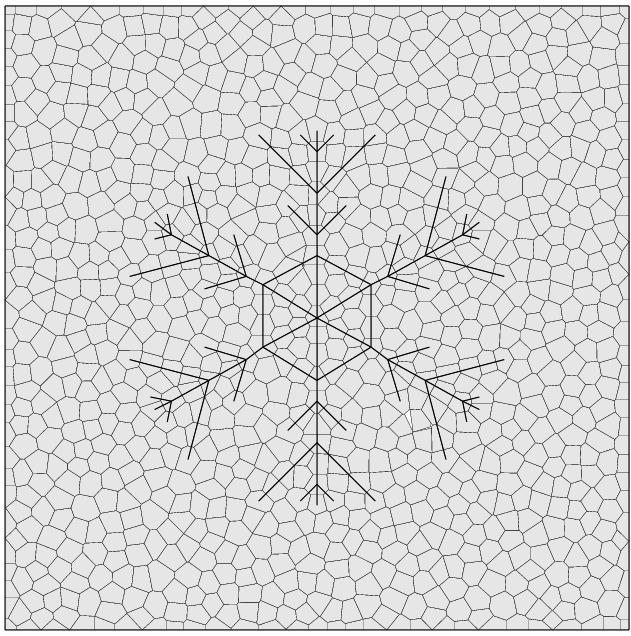
\includegraphics[height=3.7cm]{./ebeida/snowflake_voronoi.png}}$\,$
{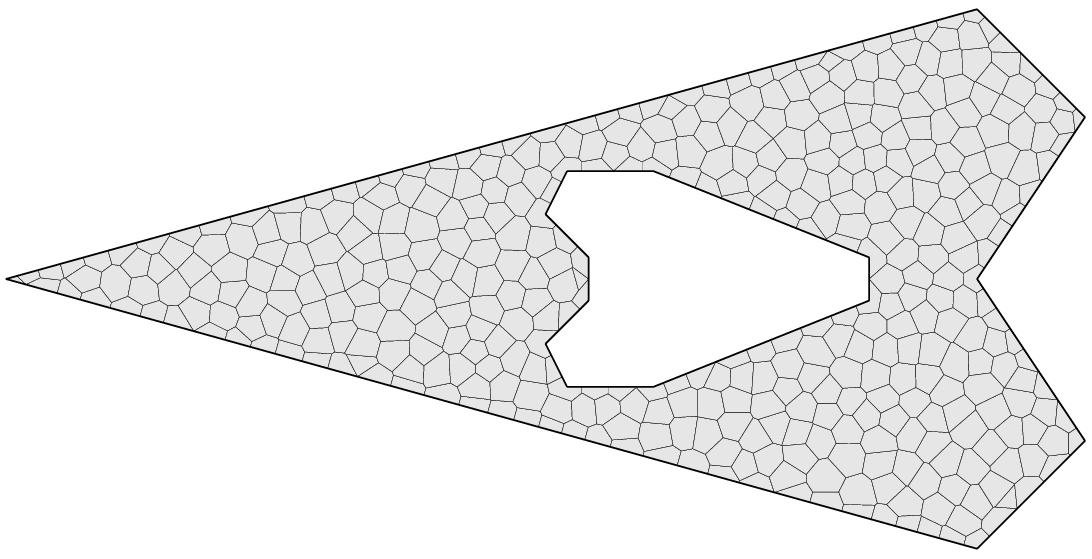
\includegraphics[height=3.7cm]{./ebeida/wedge_voronoi.png}} $\,$
{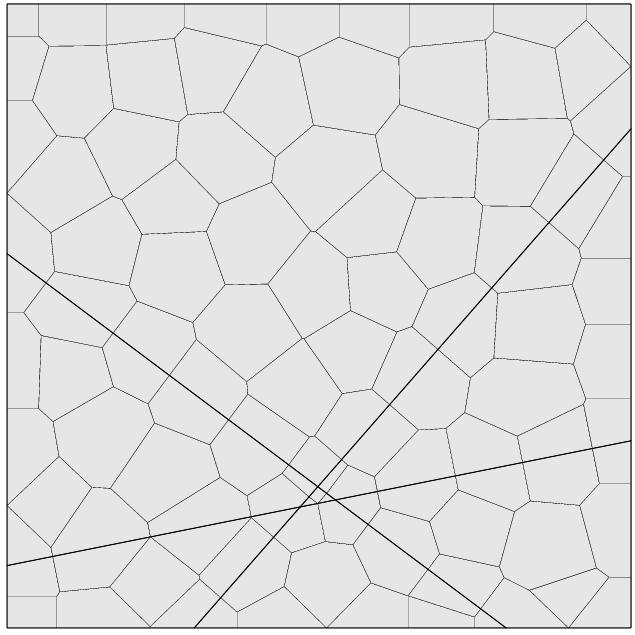
\includegraphics[height=3.7cm]{./ebeida/cracks_voronoi.png}}
\caption{Conforming Voronoi Tessellations based on a uniform distance function for a square domain with internal boundaries (left), a non-convex domain with a hole (middle) and a square domain with multiple regions in contact (right). A serial implementation of our algorithm is capable of distributing 100,000 random points/second and tessellating the output point cloud at a rate of 250,000 points/second}
\label{fig:cdt_steps}
\end{figure}\newpage
\title{Finite Element Analysis of Laser Modes within Photonic Random Media}
\author{} \institute{}
\tocauthor{\underline{G.~Fujii}, T.~Ueta}
\maketitle

\begin{center}
{\large \underline{Garuda Fujii},  Toshiro Matsumoto, Toru Takahashi}\\
Department of Mechanical Science and Engineering, Nagoya University\\
{\tt g\_fujii@nuem.nagoya-u.ac.jp}\\
\vspace{4mm}

{\large Tsuyoshi Ueta}\\
Institute of Media and Information Technology, Chiba University\\
{\tt ueta@faculty.chiba-u.jp}
\end{center}

\section*{Abstract}
Since the first experimental observation of laser action in photonic random media \cite{Lawandy}, such amplifications of light called `random laser' \cite{Wiersma} have been investigated vigorously using numerical methods \cite{Vanneste,Sebbah} as well as experimental ones \cite{Cao}.

The finite-difference time-domain (FDTD) method has been widely used for solving Maxwell's equations to simulate laser oscillations by which the electromagnetic field intensity is extremely enhanced in random media. It is, however, difficult to accomplish accurate computations by means of FDTD because of the staircase-like errors which occur on each interface of dielectric material \cite{Akyurtlu}.

On the other hand, such errors are never observed in FEM analyses because of the accurate interpolation of the shapes of the random media, hence FEM is more  advantageous for accurate calculations. In this study, the random laser action is investigated by node-base FEM calculations of the Poynting vectors emitted from the system in the case of TM mode. We use perfectly matched layer (PML) absorbing boundary condition to simulate open region scattering problem. The population inversion density within a two-dimensional random medium composed of optically active materials is modeled by the negative imaginary part of their dielectric constant \cite{Sakoda}.

\bibliographystyle{plain}
\begin{thebibliography}{10}
\bibitem{Lawandy}
{\sc N.~M.~Lawandy, R.~M.~Balachandran, A.~S.~L.~Gomes and E.~Sauvain}. {Laser action in strongly scattering media}. Nature 368 (1994), pp.~436--438.

\bibitem{Wiersma}
{\sc D.~S.~Wiersma, M.~P.~van ~Albada, and Ad.~Lagendijk}. {Random laser?}. Nature 373 (1995), pp.~203--204.

\bibitem{Vanneste}
{\sc  C.~Vanneste and P.~Sebbah}. {Selective Excitation of Localized Modes in Active  Random Media}. Phys. Rev. Lett. 87 (2001), pp.~183903-1--183903-4.

\bibitem{Sebbah}
{\sc P.~Sebbah and C.~Vanneste}. {Random laser in the localized regime}. Phys. Rev. B 66 (2002), pp.~144202-1--144202-9.

\bibitem{Cao}
{\sc  H.~Cao, J.~Y.~Xu, S.~H.~Chang and S.~T.~Ho}. {Transition from amplified spontaneous emission to laser action in strongly scattering media}. Phys. Rev. E 61 (2000), pp.~1985--1989.

\bibitem{Akyurtlu}
{\sc A.~Akyurtlu, D.~H.~Werner, V.~Veremey, D.~J.~Steich and K.~Aydin}. {Staircasing Errors in FDTD at an Air-Dielectric Interface}. J. Lightwave Tech. 17 (1999), pp.~2161--2169.

\bibitem{Sakoda}
{\sc K.~Sakoda, K.~Ohtaka and T.~Ueta}. {Low-threshold laser oscillation due to group-velocity anomaly peculiar to two- and three-dimensional photonic crystals}. Opt. Express 4 (1999), pp.481-489.
\end{thebibliography}\newpage
\title{An a Posteriori Error Estimator for $hp$-Adaptive Discontinuous Galerkin Methods for Elliptic Eigenvalue Problems}
\author{} \institute{}
\tocauthor{\underline{S.~Giani}, E.~Hall}
\maketitle

\begin{center}
{\large \underline {Stefano Giani}, Edward Hall}\\
The University of Nottingham\\
{\tt stefano.giani@nottingham.ac.uk, edward.hall@nottingham.ac.uk}
\end{center}

\section*{Abstract}
In this talk we present a residual-based a posteriori error estimator for $hp$-adaptive discontinuous Galerkin (DG) methods for elliptic eigenvalue problems. In particular we use as a model problem the Laplace eigenvalue problem on bounded domains in $\mathbb{R}^d$, $d=2,3$, with homogeneous Dirichlet boundary conditions. The same kind of error estimator can be easily extended to more complicated elliptic eigenvalue problems.

We prove the reliability and efficiency of our error estimator. The reliability ensures that,  up to a constant and to asymptotic high order terms, the error estimator gives rise to an a posteriori error bound for both eigenvalues and eigenfunctions, on the other hand, the efficiency ensures that, up to a constant and to asymptotic high order terms, the true error bounds the error estimator. Together these two results ensures that the error estimator is linearly proportional to the true error, up to higher order terms. The ratio of the constants in the upper and lower bounds is independent of both the local mesh sizes and the local polynomial degrees. 

We apply our error estimator in an $hp$-adaptive refinement algorithm and illustrate its practical performance in a series of numerical examples. 

\bibliographystyle{plain}
\begin{thebibliography}{10}
\bibitem{paola_paper}
{\sc P.~Antonietti, A.~Buffa, and I.~Perugia}. {Discontinuous Galerkin approximation of the Laplace eigenproblem}. J. Comput. Appl. Math. 204 (2007), pp.~317--333. 

\bibitem{CHHeig}
{\sc K.A.~Cliffe, E.~Hall, and P.~Houston}. {Adaptive Discontinuous {G}alerkin Methods for Eigenvalue Problems arising in Incompressible Fluid Flows}. SIAM J. Sci. Comput. 31 (2010), pp.~4607--4632.

\bibitem{Houstonlift}
{\sc P.~Houston, D.~Sch\"{o}tzau, and T.~Wihler}. {Energy norm a-posteriori error estimation of hp-adaptive discontinuous Galerkin methods for elliptic problems}. Math. Models Methods Appl. Sci. 17 (2001), pp.~33--62.

\bibitem{HoustonSuliWihler08}
{\sc P.~Houston, E.~S\"{u}li, and T.~Wihler}. {A-posteriori error analysis of $hp$-version discontinous {G}alerkin finite-element methods for second-order quasi-linear elliptic {PDEs}}.
IMA J. Numer. Anal. 28 (2008), pp.~245--273. 

\bibitem{perugia}
{\sc I.~Perugia, and D.~Sch\"{o}tzau}. {An $hp$-analysis for the local discontinuous Gelrkin method for diffusion problems}. J. Sci. Comput. 17 (2001), pp.~561--571.

\bibitem{zhu}
{\sc L.~Zhu, S.~Giani, P.~Houston, and D.~Schoetzau}. {Energy norm a-posteriori error estimation for hp-adaptive discontinuous Galerkin methods for elliptic problems in three dimensions}. M3AS 0 (2011), pp.~1-40.
M3AS  (2009). 
\end{thebibliography}\newpage
\title{Finite Volume/Element Equivalence for the Euler Equations in the Cylindrical and Spherical References}
\author{} \institute{}
\tocauthor{D.~Santis, G.~Geraci, \underline{A.~Guardone}}
\maketitle

\begin{center}
{\large Dante De Santis, Gianluca Geraci}\\
INRIA Bordeaux--Sud-Ouest, \`Equipe-projet Bacchus, Cours de la Lib\'eration\\
{\tt dante.de\_santis@inria.fr, gianluca.geraci@inria.fr}\\
\vspace{4mm}

{\large \underline{Alberto Guardone}}\\
Dipartimento di Ingegneria Aerospaziale, Politecnico di Milano\\
{\tt alberto.guardone@polimi.it}
\end{center}

\section*{Abstract}
A unified description of finite volume and finite element discretizations is proposed for the solution of the compressible Euler equations over unstructured grids in cylindrical and spherical coordinates. The method moves from suitable equivalence conditions linking finite element integrals  to the corresponding finite volume metrics, such as the cell volume or the integrated normals. The equivalence conditions were derived here without introducing any approximation and allow to determine all needed finite volume metric quantities from finite element ones \cite{selmin,ddga}. Numerical simulations are presented for the explosion problem in two spatial dimensions in cylindrical and spherical coordinates, and the numerical results are compared with the one-dimensional simulation for cylindrically and spherically symmetric explosions, in which an initial discontinuity in pressure results in the formation of a diverging shock \cite{sedov}. The computed pressure and density profile agree fairly well with one-dimensional simulation in cylindrical and spherical symmetry over a very fine grid. For the implosion problem, numerical simulations include also the effect of the presence of cylindrical obstacles in the flow field, which have been recently proposed as a mean to modify the shape of a cylindrical converging shock to increase the shock front stability in experimental studies on the sonoluminescence effect. Spherical shock waves are also considered and the modification to the shock geometry due to the presence of a spherical obstacle is evaluated numerically and compared to its cylindrical counterpart \cite{chenal}.

\bibliographystyle{plain}
\begin{thebibliography}{10}
\bibitem{selmin}
{\sc V.~Selmin}. {The node-centred finite volume approach: bridge between finite differences and finite elements}. Comp. Meth. Appl. Mech. Engng., 102 (1993), pp.~107--138.

\bibitem{ddga}
{\sc D.~De Santis, G.~Geraci, and A.~Guardone}. {Equivalence conditions for finite volume/ element discretizations in cylindrical coordinates}. V European Conference on Computational Fluid Dynamics ECCOMAS CFD (2010)

\bibitem{sedov}
{\sc L.~I.~Sedov}. {Similarity and dimensional methods in mechanics}. Academic Press (1959)
	
\bibitem{chenal}
{\sc H.~B.~Chen, L.~Zhang, and E.~Panarella}. {Stability of imploding spherical shock waves}. Journal of Fusion Energy, 14 (1995), pp.~389--392
\end{thebibliography}\newpage


% *****************************
% *   YOUR TEXT STARTS HERE   *
% *****************************

\title{On $hp$-Adaptive Solution of Complete Electrode Model Forward Problems of Electrical Impedance Tomography}
\author{} \institute{} % Intentionally left blank
\tocauthor{\underline{Harri Hakula}, Nuutti Hyv�nen, Tomi Tuominen}
\maketitle
\begin{center}
{\large \underline{Harri Hakula}}\\
Aalto University School of Science and Technology\\
Institute of Mathematics\\
Otakaari 1 \\
FIN-00076 Aalto\\
{\tt Harri.Hakula@tkk.fi}\\
\vspace{4mm} % Use this space when including 3rd author
{\large Nuutti Hyv�nen}\\
{\tt nhyvonen@math.tkk.fi} \\
\vspace{4mm} % Use this space when including 3rd author
{\large Tomi Tuominen}\\
{\tt tatuomin@math.tkk.fi}
\end{center}

\section*{Abstract}
In this paper we discuss the use of $hp$-adaptive methods of Houston \& S\"uli-type \cite{HT} 
within our own Mathematica implementation in Complete Electrode Model
(CEM) forward problems  of electrical impedance tomography \cite{LHH}. CEM problems are diffusion problems with Robin-type boundary
conditions over parts of the boundary, the electrodes. Inside the domain there are regions, 
inclusions, where
the diffusion or conductivity coefficient varies from the default value.
The task is to simulate voltage measurements with and without
inclusions on the electrodes when a given current pattern is fed through electrode pairs.
Using these potentials, which can be measured in practice, reconstructions of the conductivity can be computed.
For an $N$-electrode configuration with inclusions there are $N-1$ different forward problems to solve.
We focus on strategies for solving this problem set accurately and efficiently.
\vspace{-8mm}
\begin{figure}[h]
\centering
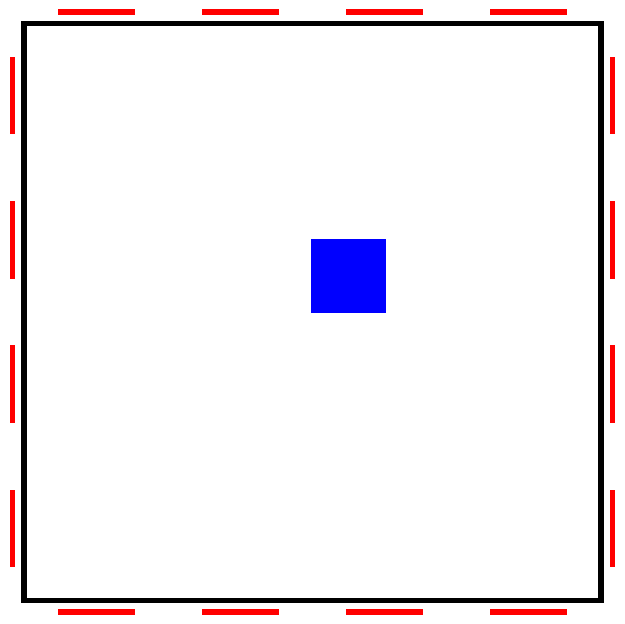
\includegraphics[width=0.15\textwidth]{domain}\qquad
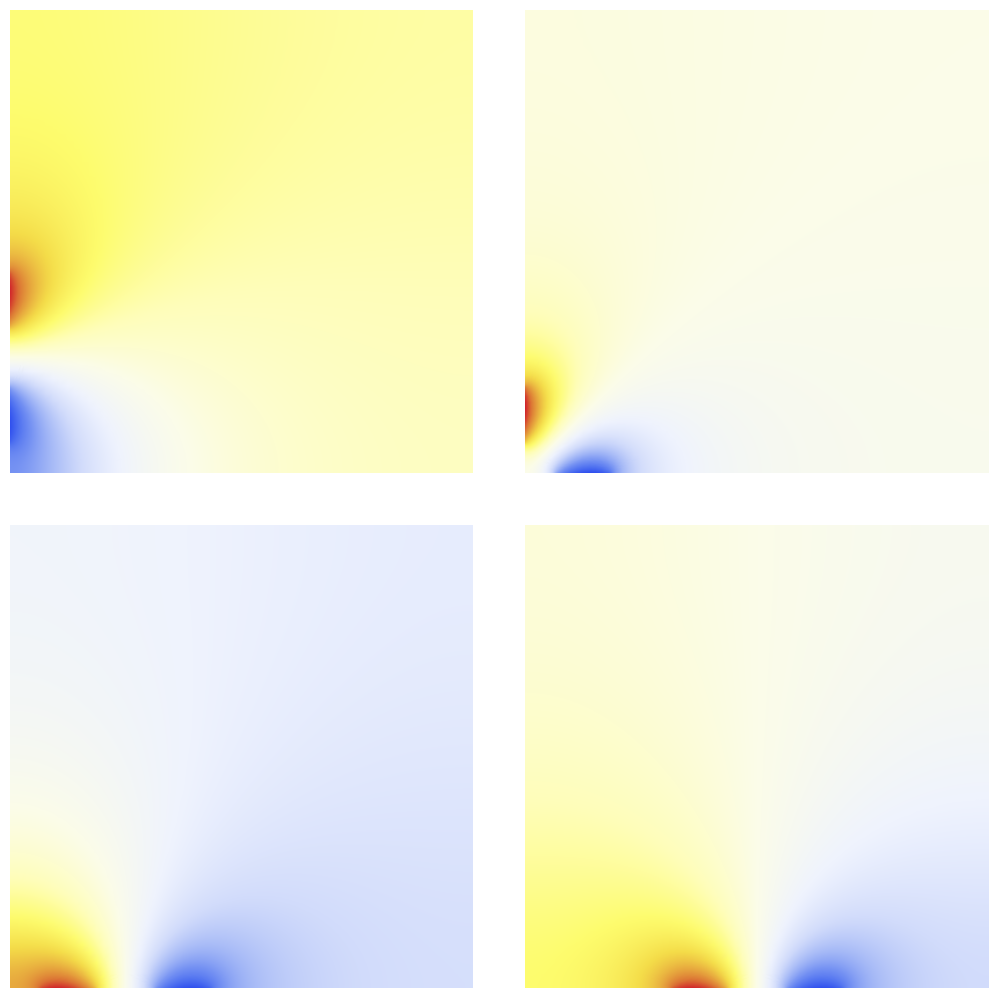
\includegraphics[width=0.16\textwidth]{potentials}\qquad
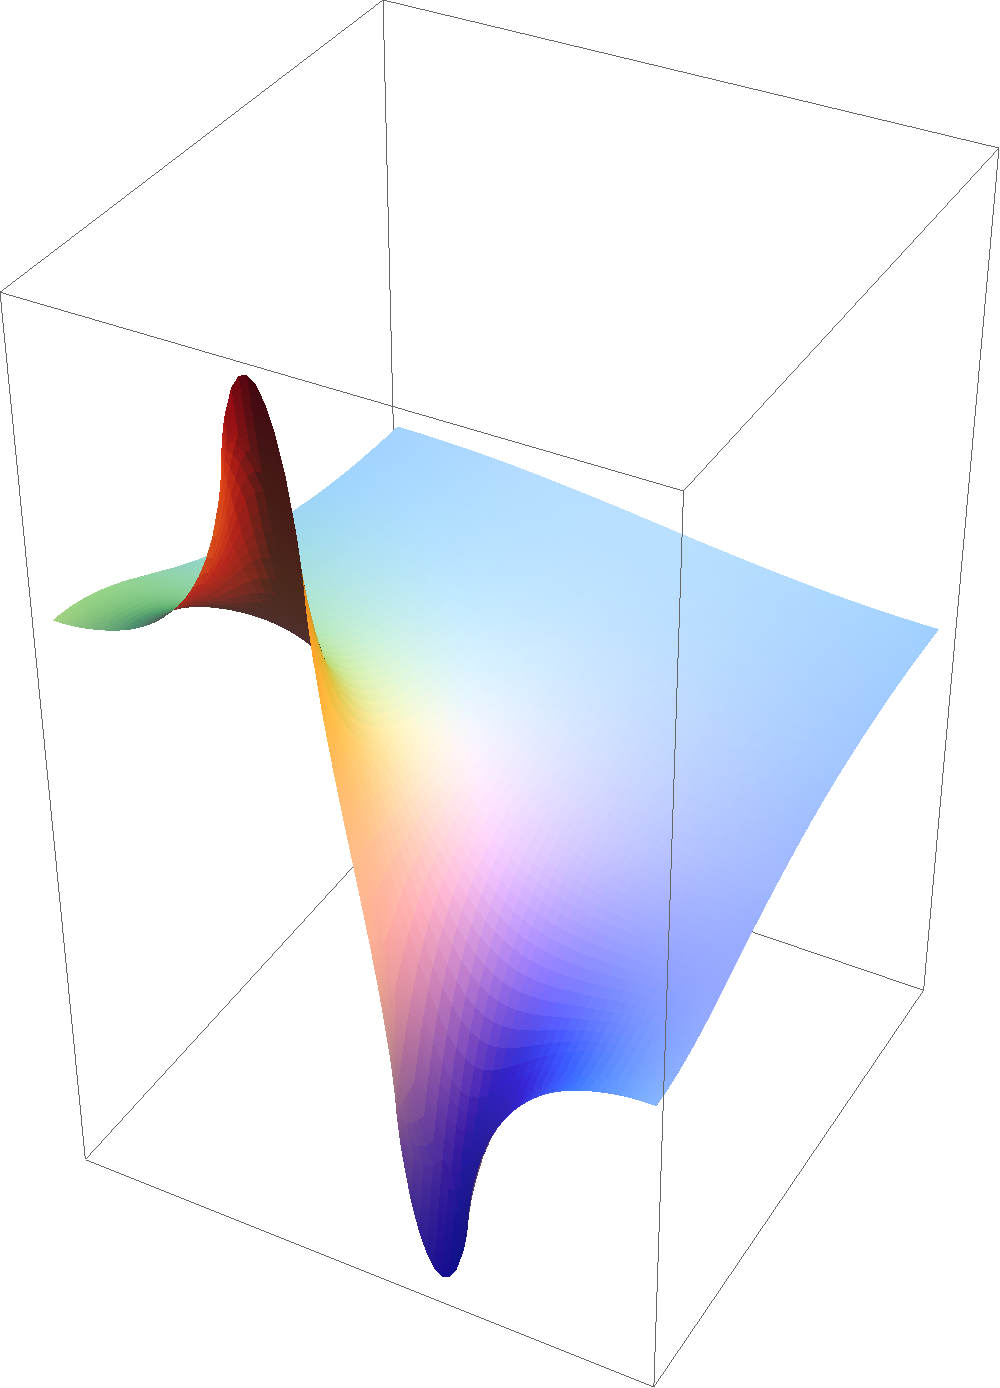
\includegraphics[height=1.25in]{potential3d}\qquad
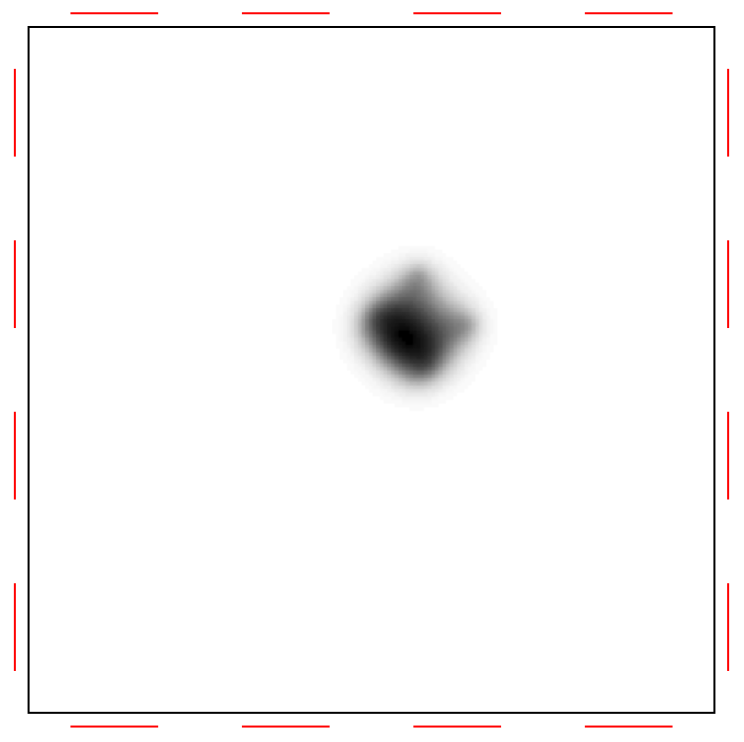
\includegraphics[width=0.15\textwidth]{reconstruction}\newline
\caption{Domain with electrodes and inclusion. Electrode pair potentials (2D\&3D). Reconstruction \cite{LHH}.}%
\label{fig}
\end{figure}
\vspace{-4mm}
\bibliographystyle{plain}
\begin{thebibliography}{10}
\bibitem{LHH} {\sc A.~Lechleiter, N.~Hyv�nen, H.~Hakula}, 
{The factorization method applied to the complete electrode model of impedance tomography}. 
SIAM Journal on Applied Mathematics, 68, pp.~1097--1121 (2008).
\bibitem{HT} {\sc H.~Hakula and T.Tuominen}, IOP Conf. Ser.: Mater. Sci. Eng. 10 012163
\end{thebibliography}

% ***************************
% *   YOUR TEXT ENDS HERE   *
% ***************************
\newpage
\title{Development of a Reactor System Analysis Code using TRILINOS}
\author{} \institute{}
\tocauthor{\underline{Glen Hansen}, Vincent Mousseau}

\begin{center}

\textbf{\Large Development of a Reactor System Analysis Code using TRILINOS}\\
\vspace{10mm}
{\large \underline{Glen Hansen}, Vincent Mousseau}\\
Idaho National Laboratory\\
{\tt Glen.Hansen@inl.gov, Vincent.Mousseau@inl.gov}

\end{center}

\section*{Abstract}

This presentation gives an overview of the development of RELAP6, a reactor thermal-hydraulics code that is based on the TRILINOS multiphysics framework from Sandia National Laboratories (\url{http://trilinos.sandia.gov}). The software constructs a dynamic rendition of the reactor facility geometry using models from component libraries and input files. The components interconnect to form a simple graph, where each component supports the required degrees of freedom (DOF) needed to support the spatial resolution needed for the analysis of the component's thermal-hydraulic behavior. The component DOF are assembled together with an ordering determined by the connectivity of the graph to form a vector of nonlinear algebraic equations.  The component graph can construct an initial condition vector given the initial state of the components, or can create a residual vector that is valid for any time state of the system. These initial conditions and system residual is used by TRILINOS' NOX nonlinear solver, various linear solvers and preconditioner packages, to obtain the state of the system each time step. Typically, this provides an implicit Jacobian-free Newton Krylov solution method that provides for stable, parallel system simulation given the user's choice of time step.

The software system leverages the CMAKE build system within TRILINOS and the CTEST testing system for regression testing. Details of the software architecture, capabilities, and design strategy will be discussed in detail.

\bibliographystyle{plain}
\begin{thebibliography}{1}

\bibitem{gaston09a}
D.~Gaston, G.~Hansen, S.~Kadioglu, D.~Knoll, C.~Newman, H.~Park, C.~Permann, and W.~Taitano.
\newblock Parallel multiphysics algorithms and software for computational nuclear engineering.
\newblock {\em Journal of Physics: Conference Series}, 180(1):012012, 2009.

\bibitem{pope:09}
M.~A. Pope and V.~A. Mousseau.
\newblock Accuracy and efficiency of a coupled neutronics and thermal hydraulics model.
\newblock {\em Nuclear Engineering and Technology}, 41(7):885--892, 2009.

\end{thebibliography}\newpage
\title{Reduced-Order Modeling of Two-Phase Flow Hydraulics using Orthonormal Wavelets}
\author{} \institute{}
\tocauthor{M.~Hernandez}
\maketitle

\begin{center}
{\large \underline{Miguel Hernandez IV}, Leticia Velazquez}\\
Department of Mathematical Sciences, The University of Texas at El Paso\\
{\tt \{miguelher,leti\}@utep.edu}\\
\end{center}

\section*{Abstract}
We present the numerical performance of the solution to nonlinear least-squares problems with reduced-order models using orthonormal wavelets.  The reduced-order wavelet modeling scheme is tested on a two-phase flow hydraulics problem using the Proteus Adaptive Hydraulics Modeling System (previously known as the Python Adaptive Hydraulics Modeling System [PyADH]) developed by the U.S. Army Corps of Engineers, Engineer Research and Development Center, Coastal and Hydraulics Laboratory.  Using Proteus, the goal is to estimate the unknown permeability field such that the difference in pressure between the model and the observed behavior of the system is minimized.

Solutions to the nonlinear least-squares problems with reduced-order models will be obtained using the Simultaneous Perturbation Stochastic Approximation (SPSA) algorithm, a stochastic steepest descent direction algorithm.  In this work, the wavelets used for model order reduction include the Daubechies, Coiflet, and Symlet families of wavelets.  In addition to a comparison of the various orthonormal wavelet families, an analysis of the performance of each at different levels of decomposition will also be discussed.

\bibliographystyle{plain}
\begin{thebibliography}{10}
\bibitem{MHWaveletModel}
{\sc M.~Hernandez~IV and L.~Velazquez and M.~Argaez}. {A Comparison of Wavelet-Based Schemes for Parameter Estimation}. Proceedings of the IEEE 2010 Users Group Conference. (2010)

\bibitem{NumTestParam}
{\sc L.~Velazquez and M.~Argaez and C.~Quintero}. {Numerical Testing of Parameterization Schemes for Solving Parameter Estimation Problems.} Proceedings of the 26th Army Science Conference (2008)
\end{thebibliography}\newpage
\title{Implicit Discontinuous Galerkin Methods for Parabolic Problems}
\author{} \institute{}
\tocauthor{\underline{J.~J.~Heys}, G.~D.~Vo, G.~Hansen}
\maketitle

\begin{center}
{\large \underline{Jeffrey J. Heys}}\\
Chemical and Biological Engineering, Montana State University\\
{\tt jeff.heys@gmail.com}\\
\vspace{4mm}

{\large Garret D. Vo}\\
Mechanical Engineering, Montana State University\\
{\tt garretvo19@gmail.com}\\
\vspace{4mm}

{\large Glen Hansen}\\
Multiphysics Methods Group, Idaho National Laboratory\\
{\tt Glen.Hansen@inl.gov}
\end{center}

\section*{Abstract}
Discontinuous Galerkin (DG) methods have the potential to combine the stable upwinding of finite volume methods with the accuracy and efficiency of high-order finite element methods.  Much of the development of DG algorithms has focus on explicit time stepping and hyperbolic equations~\cite{HesWar2010}.  In multiphysics applications, however, it is important to have the time step size flexibility allowed by implicit time stepping, and, in many cases, the equations of interest are parabolic equations, such as the advection-diffusion equation or transitional Navier-Stokes equations.  This talk will describe the derivation and implementation of implicit DG methods for parabolic problems with a focus on comparing these DG methods to traditional implicit Galerkin finite element methods in terms of both accuracy and computational cost.  The test problems for the comparison include the heat equation, advection-diffusion equation, viscous Burger's equation, and the Navier-Stokes equations.  Appealingly, the approximation spaces for velocity and pressure can be chosen almost arbitrarily with DG methods when solving the Stokes or Navier-Stokes system~\cite{CocKanSch2002}.  In order to provide a common platform for the comparison and because future development will focus on parallel implementation, the Trilinos library is used throughout the development of the implicit DG algorithms.  Previous work has shown that SA multigrid algorithms, like those available in Trilinos, can potentially give optimal scalability for DG operators~\cite{OlsSch2010}.

\bibliographystyle{plain}
\begin{thebibliography}{10}
\bibitem{HesWar2010}
{\sc J.S.~Hesthaven and T. Warburton}. {Nodal discontinuous Galerkin methods:  algorithms, analysis, and applications}. Vol.~54 in Texts in Applied Mathematics, Springer, New York, 2010.

\bibitem{CocKanSch2002}
{\sc R.~Cockburn, G. Kanschat, D. Schotzau, and C. Schwab}. {Local discontinuous Galerkin methods for the stokes system}. SIAM J.~Numer.~Anal. 40 (2002), pp.~319--343.

\bibitem{OlsSch2010}
{\sc L.N.~Olson and J.B. Schroder}. {Smoothed aggregation for Helmholtz problems}. Numer.~Lin.~Alg.~Appl. 
17 (2010), pp. 361-386. 
\end{thebibliography}\newpage


% *****************************
% *   YOUR TEXT STARTS HERE   *
% *****************************

\title{Vaporization and Combustion of Droplet Clusters in Zero Gravity Environment }
\author{} \institute{} % Intentionally left blank
\tocauthor{Irina Ciobanescu Husanu} %, \underline{Radian Belu}}
\maketitle
\begin{center}
{\large \underline{Irina Ciobanescu Husanu}}\\
Drexel University, 3001 Market Street, Philadelphia, PA 19104\\
{\tt inc22@drexel.edu}\\
\vspace{4mm} % Use this space when including 3rd author
{\large Radian Belu}\\
Drexel University, 3001 Market Street, Philadelphia, PA 19104\\
{\tt rbelu@dri.edu}
\end{center}

\section*{Abstract}
Isolated drop and drop array studies are common methods to isolate and investigate the effects of many of the complexities that enter into the drop combustion process. While the combustion of small drops (1 - 100 micro m diameters) is not greatly affected by buoyancy, these drops are difficult to observe. Microgravity environments are required to allow larger drops to be studied while minimizing or eliminating the confounding effects of buoyancy[1],[2]. Even with the large number of isolated droplet, droplet array, and spray studies that have been conducted in recent years, the extrapolation of the results from droplet array studies to spray flames is difficult since even the simplest spray systems introduce complexities of multi-disperse drop sizes and drop-drop interactions, coupled with more complicated fluid dynamics. Fiber-supported droplet array studies attempt to bridge the gap between individual group combustion and spray flames yet they, too, are limited because the fiber interactions introduce additional unknowns into the problem. The objective of this paper is to study the vaporization of well-characterized clusters in microgravity environment using direct numerical simulation. The research investigates droplet interactions during vaporization of clusters of droplets of different sizes and asymmetric three-dimensional configurations in zero gravity environments for low relative Reynolds numbers. The numerical simulation accounts for variable thermo-physical properties, includes the gas-phase radiative transfer for finite rate reaction and simulates the variation of the fuel mass flow rate with the radius of the droplets in the cluster. Mass burning rates are calculated for each droplet in an array and compared to mass burning rate of similar single droplet, the ratio of these two being a correction factor that depends on droplet diameters and droplets interspacing in cluster. Preliminary data obtained with proposed method provided results consistent with and in qualitative agreement with single droplet combustion theories[1]. These simulations may support future possible microgravity experiments. Using this system, dilute and dense clusters can be created and stabilized before combustion is begun allowing the spectrum of droplet interactions during combustion to be observed and quantified. 
\bibliographystyle{plain}
\begin{thebibliography}{10}
\bibitem{AnnamalaiRyan93}
{\sc K.~Annamalai and W.~Ryan}. {Evaporation of Arrays of Drops Using the Point Source Method}. ASME Publications, Emerging Energy Technology, PD vol. 50 (1993)
 \bibitem{MoriueaMikamiKojimaEigenbrod05}
{\sc O.~Moriuea, M.~Mikami, N.~Kojima, and C.~Eigenbrod}. {Numerical simulations of the ignition of n-heptane droplets in the transition diameter range from heterogeneous to homogeneous ignition}. Proc. of Comb. Inst. 30 (2005)

\end{thebibliography}
\newpage
\title{Finite element simulation of trocar insertion into human abdominal tissue}
\author{} \institute{}
\tocauthor{\underline{P.~Chavan}, Y.~W.~Seo}
\maketitle

\begin{center}
{\large \underline{Priyvardhan Chavan}, Yong Won Seo, Thenkurussi Kesavdas}\\
{\large Virtual Reality labs, State University of New York at Buffalo}\\
{\tt ppchavan@buffalo.edu, yongwons@buffalo.edu, kesh@buffalo.edu}
\end{center}

\section*{Abstract}
Trocar insertion, the first step to most micro surgery procedures is a difficult procedure to learn and practice because procedure is carried out almost entirely without any visual feedback of the organs underlying the tissue being punctured. A majority of injuries is attributed to the excessive use of force by the surgeon. Hence, the current research in Virtual reality lab is focused on simulating the trocar insertion procedure, in real time using advanced simulation techniques and develops a trocar insertion simulator for surgeon skill enhancement. In this paper, we present the results of our preliminary analysis of the problem, carried out using non linear FEM solver. The purpose of this analysis is to simulate the problem realistically with different material models of increasing complexity. The results of the analysis gives an idea about stress distribution pattern at the point of insertion, maximum stress developed in the vicinity of penetration and correlation between different trocar design factors and stress patterns in the vicinity of trocar insertion. We intend to use this information to construct a haptic simulator for surgeon skill training.

\bibliographystyle{plain}
\begin{thebibliography}{10}
\bibitem{KesavdasT2005}
{\sc Kesavdas T., Srimathveeravalli G., Arulesan V.}. {Parametric modeling and simulation of trocar insertion procedure}. Studies in Health Technology Inform, 2005, pp 119- 252-4

\bibitem{Brummer2008}
{\sc Brummer V., Carnahan H., Okrainec A., Dubrowski A.}. {Trocar insertion: the neglected task of VR simulation}. Medicine Meets Virtual Reality 16, J.D. Westwood et al. (Eds.), IOS Press, 2008

\bibitem{Okrainec2009}
{\sc Okrainec A., Farcas M., Henao O., Choy I., Green J., Fotoohi M., Leslie R., Wight D., Karam P., Gonzalez N., Apkarian J.}.
\newblock Development of a Virtual Reality Haptic Veress Needle Insertion Simulator for Surgical Skills Training
\newblock Medicine Meets Virtual Reality 17, J.D. Westwood et al. (Eds.), IOS Press, 2009

\bibitem{Shafer2006}
{\sc Shafer D., Khajanchee Y., Wong J. and Swanström L.}.
\newblock Comparison of Five Different Abdominal Access Trocar Systems: Analysis of Insertion Force, Removal Force, and Defect Size
\newblock Surgical Innovation, Volume 13 Number 3, September 2006, pp 183-189

\bibitem{SNg2003}
{\sc Ng P.S., Singh Sahota D., Yuen P.}.
\newblock Measurement of Trocar Insertion Force Using a Piezoelectric Transducer
\newblock Journal of the American Association of Gynecologic Laparoscopists, volume 10, issue 4, November 2003, pp 534-538
\end{thebibliography}\newpage
\title{Simulation of shock tube flows with an adaptive conservative scheme}
\author{} \institute{}
\tocauthor{\underline{Dario Isola}, Alberto Guardone}

\begin{center}

\textbf{\Large Simulation of shock tube flows with an adaptive conservative scheme}\\
\vspace{10mm}
{\large Dario Isola, Alberto Guardone}\\
Dipartimento di Ing. Aerospaziale - Politecnico di Milano, Via La Masa 34, 20156, Milano, Italy. \\
{\tt isola@aero.polimi.it, guardone@aero.polimi.it}

\end{center}

\section*{Abstract}

The numerical simulation of two-dimensional shock tube flows can be particularly challenging since, even in simple geometries, very complex unsteady flows can develop~\cite{Woodward-Colella-1984}. A quite common feature of such flows is the presence of moving shocks separating regions where the flow is substantially uniform. To reduce the computational burden and improve the overall accuracy of the solution, mesh adaptation techniques can be adopted to increase the grid spacing only where it is required~\cite{Naderi-Darbandi-Rahni-2010}.  In the present work a Finite-Volume solver for the Arbitrary Lagrangian-Eulerian (ALE) formulation of the Euler equations over two-dimensional adaptive grids~\cite{Forestieri-Isola-Marulli-Guardone-Quaranta-2010} is adopted to perform unsteady flow computations. The interpretation of the grid modifications as a continuous deformation of the finite volumes, resulting in a modification of the interface velocities, allows to compute the solution onto the new grid simply integrating the governing equations, without any explicit interpolation step~\cite{Isola-Guardone-Quaranta-2010}.

\begin{figure}

\centering
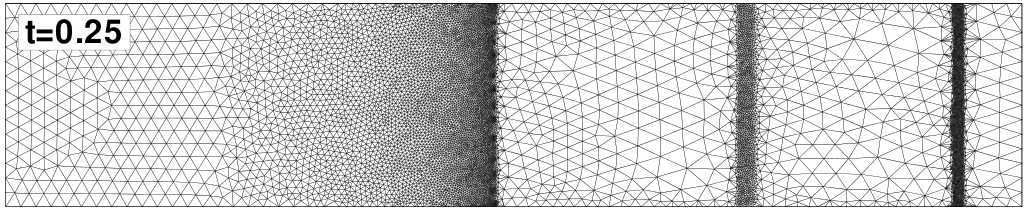
\includegraphics[height=.16\textwidth]{./isola/grid.png}
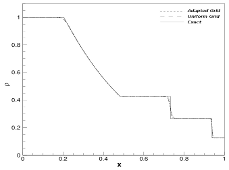
\includegraphics[height=.16\textwidth]{./isola/solution.png}
\caption{Adapted grid and density along the shock tube.}

\end{figure}

\bibliographystyle{plain}
\begin{thebibliography}{10}

\bibitem{Woodward-Colella-1984}
{\sc P.~Colella and P.~R.~Woodward}
{The numerical simulation of two-dimensional fluid flow with strong shocks}.
J. Comput. Phys. (Elsevier) 54: 115--173, (1984).
	
\bibitem{Naderi-Darbandi-Rahni-2010}
{\sc A.~Naderi, M.~Darbandi and M.~Taeibi-Rahni}
{Developing a unified FVE-ALE approach to solve unsteady fluid flow with moving boundaries}
{International Journal for Numerical Methods in Fluids, 63(1):40--68, (2010).}
	
\bibitem{Forestieri-Isola-Marulli-Guardone-Quaranta-2010}
{\sc G.~Forestieri, D.~Isola, F.~Marulli, G.~Quaranta and A.~Guardone}.
{Numerical simulation of compressible vortical flows using a conservative unstructured-grid adaptive scheme}.
2$^{nd}$ European Seminar on Coupled Problems, Pilsen, Czech Republic, (28$^{th}$ June -2$^{nd}$ July, 2010).
	
\bibitem{Isola-Guardone-Quaranta-2010}
{\sc D. Isola, A. Guardone, and G. Quaranta.}
{An {ALE} scheme without interpolation for moving domain with adaptive grids}.
AIAA 40\ensuremath{^{\textrm{th}}} Fluid Dynamics Conference and Exhibit, Chicago, IL, USA, (28 June--1 July 2010).

\end{thebibliography}\newpage
\title{Minimum Sobolev Norm Methods For Bi-Harmonic Type Equations}
\author{} \institute{}
\tocauthor{S.~Chandrasekaran, \underline{K.~R.~Jayaraman}, J.~Moffitt, M.~Gu, H.~N.~Mhaskar}
\maketitle

\begin{center}
{\large S.~Chandrasekaran, \underline{K.~R.~Jayaraman}, J.~Moffitt}\\
Department of Electrical and Computer Engineering, University of California\\
{\tt shiv@ece.ucsb.edu, jrk@ece.ucsb.edu, jmoffitt@umail.ucsb.edu}\\
\vspace{4mm}

{\large M.~Gu}\\
Department of Mathematics, University of California\\
{\tt mgu@math.berkeley.edu}\\
\vspace{4mm}

{\large H.~N.~Mhaskar}\\
Department of Mathematics, California State University\\
{\tt hmhaska@calstatela.edu}
\end{center}

\section*{Abstract}
Minimum Sobolev Norm (MSN) methods were introduced by the authors as a technique to produce higher-order interpolatory operators that suppress Runge oscillations \cite{MSN1,MSN2}. This interpolatory framework can be used to construct finite difference weights (MSN-FD weights) for solving PDEs as will be discussed in \cite{MSNFD}. One can also construct finite element (MSN-FEM) like approaches based on the MSN framework. In this article we give a brief summary of these methods and present a large set of numerical experiments to show the high efficiency, accuracy, robustness and generality of the methods. Details of meshing and mapping to assemble the grand system are discussed. We then consider the solution to equations with bi-harmonic leading terms using the MSN-FD method. Initial results obtained with the MSN-FD method for the pure bi-harmonic equation indicates it to be a very promising higher-order method. For several difficult cases accuracies of $O(10^{-8})$ were achieved with relatively coarse grids. Results of solving several classes of planar PDEs are also compared among the MSN based approaches and Finite Element Toolboxes, such as the Matlab's PDETool, Hermes \cite{Hermes} and Deal II \cite{Deal2}. Implementation issues, such as possible opportunities for parallelism, as well as implementation notes about the use of Python for the development of the above packages are discussed.

\bibliographystyle{plain}
\begin{thebibliography}{10}
\bibitem{MSN1}
{\sc S.~Chandrasekaran and H.~N.~Mhaskar}. {A construction of linear bounded interpolatory operators on the torus}, arXiv:1011.5448v1 [math.NA].

\bibitem{MSN2}
{\sc S.~Chandrasekaran, K.~R.~Jayaraman, J.~Moffitt, H.~N.~Mhaskar, and S.~Pauli}. {Minimum Sobolev Norm schemes and applications in image processing}, Proc. SPIE 7535, 753507 (2010), DOI:10.1117/12.842734.

\bibitem{MSNFD}
{\sc S.~Chandrasekaran, M.~Gu, K.~R.~Jayaraman, J.~Moffitt, H.~N.~Mhaskar}. {Higher Order Numerical Discretization Methods with Sobolev Norm Minimization}. To be submitted to The International Conference on Computational Sciences 2011.

\bibitem{Hermes}
{\sc T.~Vejchodsky, P.~Solin, M.~Zitka}. {Modular hp-FEM System HERMES and Its Application to the Maxwell's Equations}. Math. Comput. Simul. 76 (2007) 223 - 228.

\bibitem{Deal2}
{\sc W.~Bangerth, R.~Hartmann and G.~Kanschat}. {deal.II - A general-purpose object-oriented finite element library}, ACM Transactions on Mathematical Software (TOMS), Vo.33.4 (2007)
\end{thebibliography}\newpage
\title{Application Of Variational Data Assimilation To Dynamical Downscaling Of Regional Wind Energy Resources In The Western U.S.}
\author{} \institute{}
\tocauthor{\underline{J.~Jiang}, D.~Koracin, R.~Vellore, K.~Horvath, R.~Belu}
\maketitle

\begin{center}
\vspace{-6mm}
{\large \underline{Jinhua Jiang}, Darko Koracin, Ramesh Vellore}\\
Desert Research Institute, Reno 
{\tt jinhua.jiang@dri.edu}\\
\vspace{4mm}

{\large Kristian Horvath}\\
Meteorological and Hydrological Service, Zagreb 
{\tt Kristian.Horvath@dri.edu}
\vspace{4mm}

{\large Radian Belu}\\
Drexel University 
{\tt Radian.Belu@dri.edu}
\end{center}

\section*{Abstract}
Data assimilation (DA) has been widely used in mesoscale meteorological modeling. This technique merges observational data into gridded data (the first-guess fields from forecasts) to provide dynamically consistent four-dimensional datasets. For wind power forecasting, due to the non-linear relationship between wind power and wind speed, small over/under-estimations in the wind speed predictions will substantially alter the wind power assessment. In the western U.S., local topography and land-use have important effects on both wind speed and wind direction. In order to describe orographical flows or diurnal circulations, a fine spatial and temporal resolution is necessary for simulating the local/regional-scale wind characteristics, as well as for better assessments of regional wind energy resources over complex terrain. 

In this study, three-dimensional variational data assimilation is applied to short-term wind and wind power predictions with the Weather Research and Forecasting (WRF) model and WRFVar , its data assimilation module (Paegle et al. 1997, Barker et al. 2003),. The observational data used for DA include radiosonde data and RAWS (Remote Automated Weather Station) data covering California, Nevada, Arizona, Idaho, and Oregon. The WRF model is configured with a parent domain and seven nested domains. The horizontal resolution of the parent domain is 27 km. For the first three nested domains the horizontal resolutions are 9, 3 and 1 km, respectively, and for the four innermost domains are 333 m. The seven nested domains are initialized with the output from data assimilation for the parent domain. The preliminary numerical experiments showed that variationally assimilated datasets on the coarser domain (27 km grid) improved the forecasts in the nested domains compared to without WRFVar. The study further addresses the impact of increased horizontal resolution on the forecast skill over complex terrain. In addition, the effects of terrain and boundary conditions on the forecast skill are discussed.

\bibliographystyle{plain}
\begin{thebibliography}{10}
\bibitem{Bark04}
{\sc Barker, D. M., W. Huang, Y.-R. Guo, et al.}. {A three-dimensional variational data assimilation system for MM5: Implementation and initial results}.Monthly Weather Review. 132 (2004), pp.~897--914.

\bibitem{Paegle97}
{\sc Paegle, J., Q. Yang, and M. Wang}. {Predictability in limited area and global models}. Meteor. Atmos. Phys., 63 (1997), pp.~53--69.
\end{thebibliography}
\newpage % Prilis dlouhe
\title{Monolithic Modeling of Assembly of Induction Shrink Fits}
\author{} \institute{}
\tocauthor{\underline{P.~Karban}, F.~Mach, I.~Dole\v{z}el}
\maketitle

\begin{center}
{\large \underline{Pavel Karban}, Franti\v{s}ek Mach}\\
Faculty of Electrical Engineering, University of West Bohemia, RICE\\
{\tt karban@kte.zcu.cz, fmach@kte.zcu.cz}\\
\vspace{4mm}
{\large Ivo Dole\v{z}el}\\
Faculty of Electrical Engineering, Czech Technical University\\
{\tt dolezel@fel.cvut.cz}
\end{center}

\section*{Abstract}
Assembly of an induction shrink fit is modeled in monolithic formulation. This process is realized by induction heating of one part (usually that with higher coefficient of thermal dilatability) whose dimensions enlarge due to its thermal dilatation; another cold part is then inserted into the hole of the first part (or, vice versa, the hot part is drawn on the cold part). After consequent cooling of the whole system we obtain the shrink fit. The model of the process represents a triply coupled strongly nonlinear problem (typical by the interaction of magnetic field, temperature field and field of thermoelastic displacements) whose solution must be performed in hard-coupled formulation, otherwise the results may exhibit unacceptable errors.

Modeling of induction shrink fits is still a challenging problem and the relevant references are rather rare. Quasi-coupled formulation of the task can be found in \cite{Skopek} and \cite{Ukraine}, but only with very approximate respecting of nonlinearities. This paper treats the problem much more accurately. The authors describe its complete mathematical model consisting of three nonlinear partial differential equations and illustrate its solution by numerical computation of a typical example. The computations are carried out by codes Hermes2D and Agros2D \cite{Hermes2D} based on the finite element method of higher order of accuracy and algorithms described partly in \cite{Solin}. The solution is supplemented with the analysis of the influence of the principal nonlinearities on the accuracy of results.

This work was supported by the European Regional Development Fund and Ministry of Education, Youth and Sports of the Czech Republic under the project No. CZ.1.05/2.1.00/03.0094: Regional Innovation Centre for Electrical Engineering (RICE) and by Grant project GACR P102/11/0498.

\bibliographystyle{plain}
\begin{thebibliography}{10}

\bibitem{Skopek}
{\sc M.~Skopek, B.~Ulrych, and I.~Dole\v{z}el}. {Optimized regime of induction heating of a disk before its pressing on shaft}. IEEE Trans. on Magn. 37 (2001), pp.~3380--3383.

\bibitem{Ukraine}
{\sc I.~Dole\v{z}el, P.~Karban, B.~Ulrych, M.~Pantelyat, Y.~Matyukhin, P.~Gontarowsky, and N. Shulzhenko}. {Limit operation regimes of actuators working on principle of thermoelasticity}. IEEE Trans. on Magn. 44 (2008). pp.~810--813.

\bibitem{Hermes2D}
{http://hpfem.org}.

\bibitem{Solin}
{\sc P.~Solin, J.~Cerveny, L.~Dubcova, and D.~Andrs}. {Monolithic discretization of linear thermoelasticity problems via adaptive multimesh \textit{hp}-FEM}. J. Comput. Appl. Math. 234 (2010), pp.~2350--2357.
\end{thebibliography}\newpage


% *****************************
% *   YOUR TEXT STARTS HERE   *
% *****************************

\title{Multiscale Numerical Modeling of Levee Breach Processes}
\author{} \institute{} % Intentionally left blank
\tocauthor{\underline{C. E. Kees}, M. W. Farthing, I. Akkerman, and Y. Bazilevs}
\maketitle
\begin{center}
{\large \underline{C. E. Kees}}\\
US Army ERDC, Vicksburg, MS, USA\\
{\tt christopher.e.kees@usace.army.mil}\\
\vspace{4mm} % Use this space when including 3rd author
{\large M. W. Farthing}\\
US Army ERDC, Vicksburg, MS, USA\\
{\tt matthew.w.farthing@usace.army.mil}\\
\vspace{4mm} % Use this space when including 3rd author
{\large I. Akkerman}\\
US Army ERDC, Vicksburg, MS, USA\\
{\tt idoakkerman@gmail.com}\\
\vspace{4mm} % Use this space when including 3rd author
{\large Y. Bazilevs}\\
Structural Engineering, University of Caifornia, San Diego, CA, USA\\
{\tt jbazilevs@ucsd.edu}\\
\end{center}

\section*{Abstract}
One of the dominant failure modes of levees during flood and storm
surge events is erosion-based breach formation due to high velocity
flow over the back (land-side) slope.  Modeling the breaching process
numerically is challenging due to both physical and geometric
complexity that develops and evolves during the overtopping event. The
surface water flows are aerated and sediment-laden mixtures in the
supercritical and turbulent regimes. The air/water free surface may
undergo perturbations on the same order as the depth or even
topological change (breaking). Likewise the soil/fluid interface is
characterized by evolving headcuts, which are essentially moving
discontinuities in the soil surface elevation. The most widely used
models of levee breaching are nevertheless based on depth-integrated
models of flow, sediment transport, and bed morphology. In this work
our objective is to explore models with less restrictive modeling
assumptions, which have become computationally tractable due to
advances in both numerical methods and high-performance computing
hardware. In particular, we present formulations of fully
three-dimensional flow, transport, and morphological evolution for
overtopping and breaching processes and apply recently developed
finite element and level set methods to solve the governing equations
for relevant test problems.

%% Enter your abstract here. Authors of contributed lectures: Please do not 
%% exceed one page including references. References to related or 
%% competitive work are mandatory. Presenting author should be underlined. 
%% Please do not alter the internal structure of the template. Do not 
%% introduce any new definitions or commands, they cause problems during the 
%% compilation of the final Book of Abstract. The Book of Abstracts will be 
%% compiled using pdflatex. If using images, please make sure thay are
%% in PDF or PNG. Thank you!


 \bibliographystyle{plain}
 \begin{thebibliography}{10}

 \bibitem{CockburnGopalakrishnan04}
 {\sc B.~Cockburn and J.~Gopalakrishnan}. {A characterization of hybridized
   mixed methods for second order elliptic problems}. SIAM J. Numer. Anal. 42
   (2004), pp.~283--301.

 \bibitem{EwingWangYang03}
 {\sc R.~Ewing, J.~Wang, and Y.~Yang}. {A stabilized discontinuous finite
   element method for elliptic problems}. Numer. Linear Alg. Appl. 10 (2003),
   pp.~83--104.

 \bibitem{A104}
 {\sc Randolph~E. Bank, Jinchao Xu, Bin Zheng}.
 \newblock Superconvergent derivative recovery for {Lagrange} triangular
   elements of degree $p$ on unstructured grids.
 \newblock SIAM J.~Numer. Anal. 45 (2007), pp. 2032--2046. 

 \end{thebibliography}

% ***************************
% *   YOUR TEXT ENDS HERE   *
% ***************************
\newpage
\title{The Sizing and Shape Optimization of Hospital Bed Structure for Independently Seperating Left and or Right Leg to Search Minimum Mass}
\author{} \institute{}
\tocauthor{A.~Ariyarit, \underline{R.~Kittipichai}}
\maketitle

\begin{center}
{\large Atthaphon Ariyarit, \underline{Rung Kittipichai}}\\
Department of Mechanical Engineering, Faculty of Engineering, Mahidol University\\
{\tt u5013419@student.mahidol.ac.th, egrkt@mahidol.ac.th}\\
\end{center}

\section*{Abstract}
At present, there are many types of the hospital bed with various functions such as lifting the head section or leg section of the bed. Unfortunately, the hospital bed cannot lift either left or right leg. That means when the patient's left leg or right leg is broken, the hospital bed need to lift both legs. It cannot lift independently.  This work focuses on the hospital bed design for independently separating the left and or right leg  for patient's leg splint. The paper proposes an idea to search the minimum mass of hospital bed. The design problem is a combination of sizing and shape optimization of bed structure. The aim is to minimize the mass of bed structure subject to nodal displacement, stress and buckling constraints using Genetic Algorithms (GAs) as a stochastic search method.\\
The bed structure was modeled and analyzed by using Finite Element (FE) method. FE with 2-D beam element was selected and applied to the 3-D bed structure. The GAs and FE code using MATLAB program were developed to analyze the structure. The bed structure was modeled by using 54 beam elements with 38 nodes. The mass of bed structure was minimized by reducing the cross-section area of each element and changing some node position under the down force of 4,600 N and the left and right side force of 2,750 N. The structure was made of steel alloy with the safety factor of 2. The total design variables of the optimization problem were 56 variables in the sizing part and 4 variables in the shape part.  In GA procedure, the number of strings in a population and the number of generation was set to 500 and 1500, respectively. The results showed the success in searching the minimum mass whilst the stress, nodal displacement and buckling constraints were accepted. The optimum mass for the bed structure was 39.22 kg with the maximum constraint of stress in the element. Therefore, this paper demonstrates that it is possible to design the hospital bed for independently separating left and or right leg by using GAs combined with FE analysis to search the minimum mass. 

\bibliographystyle{plain}
\begin{thebibliography}{10}
\bibitem{W.M.Jenkins97}
{\sc W.~M.~ Jenkins}. {On the application of natural algorithms to structural design optimization}. Engineering Sturcture J.  Vol. 19 (1997), pp.~302--308.

\bibitem{AnnicchiaricoCerrolaza98}
{\sc W. ~Annicchiarico and M. ~Cerrolaza}. {Optimization of finite element bidimensional models: an approach based on genetic algorithms}.Finite Elements in Analysis and Design  Vol. 29 (1998), pp.~231--257.

\bibitem{CoelloChristiansen00}
{\sc C. ~A. ~Coello and A. ~D. ~Christiansen}. {Multiobjective optimization of trusses using genetic algorithms}.Computers \& Structures. Vol. 75 (2000), pp.~647--660.

\bibitem{DebGulati01}
{\sc K. ~Deb and S. ~Gulati}. {Design of truss-structures for minimum weight using genetic algorithms}. Finite Elements in Analysis and Design. Vol. 37 (2001), pp.~447--465.

\bibitem{Dow98}
{\sc J. ~O. ~Dow}. {A unified approach to the finite element method and error analysis procedure}. London: Academic Press (1998).

\bibitem{Cook89}
{\sc R. ~D. ~Cook, et al., }. {Concepts and applications of finite element analysis}.,New York: John Wiley \& Son (1989).

\bibitem{Rao05}
{\sc S. ~S. ~Rao}. {The finite element method in engineering, 4th ed}. Amsterdam: Boston, MA: Elsevier/Butterworth Heinemann (2005).

\bibitem{Shigley86}
{\sc J. ~E. ~Shigley}. {Mechanical engineering design.} London: McGraw-Hill (1986).

\bibitem{Mott92}
{\sc R. ~L. ~Mott}. {Machine elements in mechanical design}. New York: Maxwell Macmillan International (1992).

\bibitem{Holland75}
{\sc J. ~H. ~Holland}. {Adaptation in natural and artificial systems : an introductory analysis with applications to biology, control, and artificial intelligence}. Ann Arbor: University of Michigan Press (1975).

\bibitem{Goldberg89}
{\sc D. ~E. ~Goldberg}. {Genetic algorithms in search, optimization, and machine learning}. Reading: Addison-Wesley (1989).

\bibitem{Coello00}
{\sc C. ~A. ~C. ~Coello}. {Constraint-Handling using an Evolutionary Multiobjective Optimization Technique}. ," Civil Engineering and Environmental Systems. Vol. 17 (2000), pp.~319--346.

\bibitem{Bureera01}
{\sc S. ~Bureerat}. {Multidisciplinary Optimisation of Mechanical and Aerospace Systems}. the Degree of Doctor of Philosophy, Faculty of Science and Engineering, University of Manchester (2001).
\end{thebibliography}\newpage % Prilis dlouhe

% *****************************
% *   YOUR TEXT STARTS HERE   *
% *****************************

\title{Combined Adaptive Multimesh $hp$-FEM/$hp$-DG for Multiphysics 
Coupled Problems Involving Compressible Inviscid Flows}
\author{} \institute{} % Intentionally left blank
\tocauthor{Lukas Korous, \underline{Milan Hanus}}
\maketitle
\begin{center}
{\large Lukas Korous}\\
Univerzita Karlova v Praze\\
{\tt lukas.korous@gmail.com}\\
\vspace{4mm} % Use this space when including 3rd author
{\large \underline{Milan Hanus}}\\
Zapadoceska Univerzita v Plzni\\
{\tt mhanus@kma.zcu.cz}
\end{center}

\section*{Abstract}

During the last decade, Discontinuous Galerkin (DG) methods have
been studied by numerous researchers in the context of different
problems ranging from linear elliptic equations to Euler equations
of compressible inviscid flow, the latter e.g. in~\cite{1}. It is well known that DG methods
yield larger discrete problems than standard continuous finite
element methods (FEM). On the other hand, their implicit stabilization
through embedded numerical fluxes makes them particularly well
suited for hyperbolic flow problems. Thus for multiphysics problems
involving compressible flow we propose to combine the best
of both worlds: DG is used for the flow part only while standard
FEM is employed for second-order equations where it works very well.
The DG/FEM combination is carried out for arbitrary-degree elements
in a monolithic fashion, using a novel multimesh hp-FEM technology
deployed by Dr. Solin and his collaborators~\cite{2},~\cite{3}.


\bibliographystyle{plain}
\begin{thebibliography}{10}

\bibitem{1}
{\sc V. Dolejsi, M. Feistauer, C. Schwab}. {On Some Aspects of the Discontinuous Galerkin Finite Element Method for Conservation Laws}. Math. Comput. Simul. 61 (2003), pp.~333--346.

\bibitem{2}
{\sc L. Dubcova, P. Solin, J. Cerveny, P. Kus}. {Space and Time Adaptive Two-Mesh $hp$-FEM for Transient Microwave Heating Problems}. Electromagnetics, Vol. 30, Issue 1 (2010), pp.~23--40.

\bibitem{3}
{\sc P. Solin, J. Cerveny, L. Dubcova, D. Andrs}. {Monolithic Discretization of Linear Thermoelasticity Problems via Adaptive Multimesh $hp$-FEM}. J. Comput. Appl. Math 234 (2010), pp.~2350--2357.

\end{thebibliography}

% ***************************
% *   YOUR TEXT ENDS HERE   *
% ***************************
\newpage
\title{Ica Based Channel Seperation of EEG}
\author{} \institute{}
\tocauthor{\underline{S.~S.~Kumar}, B.~Kishore}
\maketitle

\begin{center}
{\large \underline{S.~Senthil Kumar}}\\
{\tt sentheeyan@yahoo.co.in}\\
\vspace{4mm}
{\large B.~Kishore}\\
{\tt bk\underline{ }7in@yahoo.com}
\end{center}

\section*{Abstract}
This project deals with the usage of Independent Component Analysis for processing EEG signal. In this proposed project we have obtained EEG signal from a normal human subject and processed through five signal processing techniques which are signal acquisition, filtering, sub sampling, running ICA and signal extraction. As a result of this process we have obtained processed EEG data from which channels responsible for performing certain specified tasks done by the normal human subject while taking EEG can be obtained. This has been obtained by undergoing certain internal threshold operations based on ICA weightage of the processed EEG signal. This project can be extended for helping handicapped people by implementing artificial parts to their body based on their EEG signal generated. In this project we have used a specified tool kit to perform EEG based operations called as “EEG LAB tool kit” which is a toolbox that can be added to MATLAB.\newpage
\title{Seepage Influence due to Joint Sealing Damaged of CRFD Built on Covering Layers}
\author{} \institute{}
\tocauthor{\underline{G.~Lei}, Z.~Shen}
\maketitle

\begin{center}
{\large \underline{Gan Lei}, Zhenzhong Shen}\\
Institude of Hydraulic Structures, Hohai University\\
{\tt ganlei2015@hhu.edu.cn, shen6627@yahoo.com.cn}
\end{center}

\section*{Abstract}
The safe operation of concrete face rock fill dam what built on covering layers depends on the integrity of its water stop system. So analyzing of seepage field inside the dam before and after joint seal damage is significant, including the research of the influence on the dam seepage behavior when the water stop of peripheral joint and slab joint damaged. In this paper, the CRFD of a specific hydropower station project was used to be as a case. The numerical analysis models for simulating the different water stop damage and failure types were established. So as to compare the dam seepage before and after the joint water stop damaged and analyze the influence mechanism how the peripheral joint and slab joint damaged affect the seepage gradient , saturated surface and seepage discharge inside the dam. Base on the presenting results, the water stop area where needed to focus on can be ascertained when the dam anti-seepage system was arranged.

\bibliographystyle{plain}
\begin{thebibliography}{10}
\bibitem{DaweiNenghuiZhankuan 04} 
{\sc Sun Dawei, Li Nenghui, and Mi Zhankuan}. {Advance and prospect on key technology of CFRD on thick alluvium deposits}. Water Power. 08(2005), pp.~67--69.

\bibitem{LiderChernovCherdantsev 04}
{\sc A.~Lider,I.~Chernov,and Y.~Cherdantsev}. {Hydrogen Permeability of Covering Layer Generated by Electron Beam Processing}. JOURNAL OF IRON AND STEEL RESEARCH INTERNATIONAL. 17(2010), pp.~77--81.

\bibitem{Xiaoli 04}
{\sc Wen Xiaoli}. {Joint sealing design of Jiudianxia CFRD}. Gansu Water Conservancy and Hydropower Technology. 03(2008), pp.~196--197.

\bibitem{Cooke 04}
{\sc J.B.~Cooke}. {Proceedings of International Symposium on High Earth-rockfill Dams}. Chinese Soeiety for Hydro-electric Engineering.01(1993).

\bibitem{Neidert 04}
{\sc S.H.~Neidert}. {Design and construetion of the Segredo conerete-faced rockfill dam }. Water Power and Dam construetion. .06(1991).

\bibitem{BaoyuZhenzhongJian 04}
{\sc Su Baoyu, Shen Zhenzhong,and Zhao Jian}. {The cut-off negative pressure method for soling filtration problems based on the theory of variational inequalities}. JOURNAL OF HYDRAULIC ENGINEERING. 03(1996), pp.~22--29.

\bibitem{ZhenzhongChunmei 04}
{\sc Shen zhenzhong and Mao Chunmei}. {Calculation of steady seepage field and Automation draw nets}. JOURNAL OF HOHAI UNIVERSITY (NATURAL SCIENCES). 22(1994), pp.~75--77.
\bibitem{Shuwen 04}
{\sc Qi Shuwen}. {Research on Calculation Method of Seepage Discharge for Complicated 3-D Seepage Flow Field Based on FEM}. Hohai University. 05(2007).

\bibitem{ZhenzhongLiqunShuwen 04}
{\sc SHEN Zhenzhong, XU Liqun,and QI Shuwen}. {A New Interpolation Meshing Method for Calculating Section Seepage Flux}. The 10th national conference on percolation mechanics. 04(2009).
\end{thebibliography}\newpage
\title{Analysis of Earthquake Response of A Face Rock-fill Dam}
\author{} \institute{}
\tocauthor{\underline{C.~Li}, Z. Shen, Y.~Jiao}
\maketitle

\begin{center}
{\large \underline{Li Chenliang}, Shen Zhenzhong}\\
Institude of Hydraulic Structures, Hohai University\\
{\tt chenliang-li@163.com, shen6627@yahoo.com.cn}
\end{center}

\section*{Abstract}
By use of the 3-dimensional dynamic non-linear FEM, the earthquake response behavior of Xigu Face Rock-fill Dam is researched in detail. The dynamic response properties of the dam are obtained at design peak acceleration of input earthquake curve, such as acceleration response, displacement response, stress response of dam body and concrete face, and displacement response of its peripheral joint and slab joint. Under an earthquake action with ten percent of exceeding probability in 50 years, the maximum acceleration reaction, displacement reaction and shear stress reaction of the dam body are 7.37m/s2, 81mm and 484kPa. The displacement response of peripheral joint and slab joint is very little. Calculation results show that the seismic stability of the dam body meets the specifications, and the design of the dam body is technically reasonable.

\bibliographystyle{plain}
\begin{thebibliography}{09}
\bibitem{XYZZSX 04}
{\sc Wen XY, Shen ZZ,and Lv SX}. {Study on Stress and Deformation Properties of Jiudianxia Concrete Face Rockfill Dam}. Journal of Hehai University (Natural Sciences ). 33(2005), pp.~42--46.

\bibitem{YZGC 04}
{\sc Dai YZ and Gu GC}. {Three-dimensional Nonlinear Analysis for Gongbo Gorge Concrete Face Rockfill Dam on the Yellow River}. Hongshui River. 20(2001), pp.~37--41.

\bibitem{GC 04}
{\sc Gu GC}. {Earthquake Engineering of Earth-Rock Fill Dams}.Hohai University Press (in Chinese). (1989).

\bibitem{SCGC 04}
{\sc Chi SC and Gu GC}. {Seismic stability Analysis of Concrete Face Rockfill Dam}. WATER RESOURSE HYDROPOWER OF NORTHEAST CHINA. 137(1995), pp.~3--5.

\bibitem{ZZMSX 04}
{\sc Shen ZZ, Ma M, and Lv SX}. {Seismic stability Analysis of Jiudianxia Concrete Face Rockfill Dam}. Conference Proceedings of First National Meeting on Hydraulic Earthquake and Disaster Prevention in China. (2006), pp.~273--278.

\bibitem{YZGC 04}
{\sc Dai YZ and  Gu GC}. {Three-dimensional Nonlinear Analysis for Gongbo Gorge Concrete Face Rockfill Dam on the Yellow River}. Hongshui River. 20(2001), pp.~37--41.

\bibitem{ZYZJ 04}
{\sc Xu ZY and Shen ZJ}. {Static and Dynamic Nonlinear Analysis and Seismic stability of High Tailing Dams}. Journal of East China Institute of Water Conservancy. 04(1980), pp.~1--17.

\bibitem{SSQYM 04}
{\sc Zhu S, Wen SQ,and Huang YM}. {Deformation and StressCalculation for A 200m High CFRD}. ournal of Hehai University (Natural Sciences ). 31(2003), pp.~631--634.

\bibitem{JMWS 04}
{\sc Zhao JM and Wang WS}. {Deformation and StressCalculation for A 200m High CFRD}. ournal of Hehai University (Natural Sciences ). 20(2001).
\end{thebibliography}\newpage
\title{A Fast Mesh-Alignment Algorithm for 2D Curvilinear Grid}
\author{} \institute{}
\tocauthor{Shengtai Li, \underline{Second Author}}

\begin{center}

\textbf{\Large A Fast Mesh-Alignment Algorithm for 2D Curvilinear Grid}\\
\vspace{10mm}
{\large\underline{Shengtai Li}, J. Mac Hyman}\\
Theoretical Division, Los Alamos National Laboratory, NM 87545, USA\\
{\tt sli@lanl.gov, hyman@lanl.gov}\\
\vspace{4mm}
{\large Patrick Knupp} \\
Applied Mathematics \& Applications Dept.
Sandia National Laboratories, 
Alberquerque, NM 87185, USA \\
{\tt pknupp@snl.gov}\\
\vspace{4mm}
{\large Mikhail Shashkov} \\
Computational Physics Division, Los Alamos National Laboratory, NM
87545, USA \\ 
{\tt shashkov@lanl.gov}

\end{center}

\section*{Abstract}

When numerically approximating physical systems with discontinuous coefficients, often the largest numerical errors are introduced in a neighborhood of the discontinuities. These errors are often greatly reduced if the grid is aligned with the discontinuities. In predicting the extent of contamination and environment danger posed by subsurface flows from hazardous waste sites, the rate and direction of underground flows is governed by discontinuities in the geomorphology of the flow field.  Numerical approximations are more accurate when the underlying grid is  aligned with the discontinuities to minimize the heterogeneity  within a grid cell.

We will present a new numerical algorithm that aligns a curvilinear grid with internal alignment curves (IACs).  These IACs can be used to delineate internal interfaces, discontinuities in material properties, internal boundaries, or major features of a flow field. Our grid generation algorithm readjusts a predefined reference grid to create a nearby grid where the mesh cell edges are aligned with the IACs.  On an aligned grid, numerical discretizations of partial differential
equations can be formulated to satisfy the interfacial relations, such as matching fluxes across the discontinuity, to  reduce the numerical errors introduced by the discontinuity.  We present  examples to demonstrate the effectiveness of the grid-alignment algorithm for multiple imbedded interfaces.   

\bibliographystyle{plain}
\begin{thebibliography}{10}

\bibitem{CockburnGopalakrishnan04}
{\sc J.M.~Hyman, P.~Knupp, S.~Li, and M.~Shashkov}. {An algorithm to align a
quadrilateral grid with internal boundary}. J. Comput. Phys. 136
(2000),  133

\end{thebibliography}\newpage
\title{Hard-coupled model of induction heating of cylindrical billets by rotation in static magnetic field}
\author{} \institute{}
\tocauthor{\underline{F.~Mach}, P.~Karban, I.~Dole\v zel}
\maketitle

\begin{center}
{\large \underline{Franti\v{s}ek Mach}, Pavel Karban}\\
Faculty of Electrical Engineering, University of West Bohemia, RICE\\
{\tt fmach@kte.zcu.cz, karban@kte.zcu.cz}\\
\vspace{4mm}

{\large Ivo Dole\v{z}el}\\
Faculty of Electrical Engineering, Czech Technical University\\
{\tt dolezel@fel.cvut.cz}
\end{center}

\section*{Abstract}
Induction heating of cylindrical billets by their rotation in static magnetic field belongs to modern and progressive technologies characterized by substantially higher efficiency in comparison with the classical processes \cite{UIE1}, \cite{UIE2}. The paper deals with the case when the static field is generated by a system of permanent magnets, thus without any losses in the field windings. Nowadays, this variant is explored very intensively mainly for billets of lower radii (one of somewhat simplified models was solved, for example, in \cite{HES}).

The mathematical model of the problem consists of two nonlinear partial differential equations describing the distribution of magnetic and temperature fields (the nonlinearities rooting in the temperature dependencies of the physical parameters of individual parts of the system). Its numerical solution is carried out by a fully adaptive higher-order finite element method in the monolithic formulation using the codes Hermes2D and Agros2D \cite{Hermes2D}. Except for the determination of the most important thermal and mechanical characteristics of heating the authors also deal with the sensitivity analysis of various nonlinearities on the results. Another comparison is performed for the results obtained on a common triangular mesh and mesh containing curvilinear elements that perfectly copies particular boundaries in the system.

This work was supported by the European Regional Development Fund and Ministry of Education, Youth and Sports of the Czech Republic under the project No. CZ.1.05/2.1.00/03.0094: Regional Innovation Center for Electrical Engineering (RICE), further by Grant project GACR P102/10/0216, and by Research Plan MSM6840770017.

\bibliographystyle{plain}
\begin{thebibliography}{10}
\bibitem{UIE1}
{\sc M.~Zlobina, B.~Nacke, and A.~Nikonarov}. {Electromagnetic and thermal analysis of induction heating of billets by rotation in DC magnetic field}. Proc. UIE Krakow, Poland (2008), pp.~21--22.

\bibitem{UIE2}
{\sc S.~Lupi and M. Forzan}. {A Promising high efficiency technology for the induction heating of aluminium billets}. Proc. UIE Krakow, Poland (2008), pp.~19--20.

\bibitem{HES}
{\sc P.~Karban, F.~Mach, and I.~Dolezel}. {Higher-order finite element modeling of rotational induction heating of nonferromagnetic cylindrical billets}. Proc. HES Padua, Italy (2010), pp.~515--522.

\bibitem{Hermes2D}
{http://hpfem.org}
\end{thebibliography}\newpage
\title{Solving a Suite of NIST Benchmark Problems with Hermes}
\author{} \institute{}
\tocauthor{\underline{Z.~Ma}, L.~Korous, E.~Santiago}
\maketitle

\begin{center}
{\large \underline{Zhonghua Ma}}\\
China University of Petroleum\\
{\tt mazhonghua83@gmail.com}\\
\vspace{4mm}

{\large Luka\v s Korous}\\
Charles University in Prague\\
{\tt lukas.korous@gmail.com}\\
\vspace{4mm}

{\large Erick Santiago}\\
University of Nevada\\
{\tt laviticus@sbcglobal.net}
\end{center}

\section*{Abstract}
Adaptive grid refinement is a critical component of algorithms for the numerical solution of partial differential equations (PDEs). The development of new algorithms and computer codes for the solution of PDEs usually involves the use of proof-of-concept test problems [1,2].

It is common to compare different algorithms using a large test set, to evaluate the algorithm's overall quality, which lies in the ability to handle all kinds of problems, and also to determine the algorithm's strengths and weaknesses.

In this paper we solve a set of benchmark problems devised by W. Mitchel at NIST [1]. The problems exhibit various types of singularities, disruptions, and oscillations.

Each of the benchmark problem is introduced, together with its exact solution. Then the solution obtained with the use of the multi-platform open source C++ library for rapid development of adaptive $hp$-FEM and $hp$-DG solvers {\sc Hermes} [3] is shown, complemented with convergence graphs and comparison of the fully anisotropic $hp$-FEM to low-order FEM in terms of convergence.

\bibliographystyle{plain}
\begin{thebibliography}{10}
\bibitem{mitchell-1}
{\sc W.~Mitchell}. {A Collection of 2D Elliptic Problems for Testing Adaptive Algorithms}. NISTIR 7668, 2010 (available online).

\bibitem{hpfem-1}
{\sc P.~Solin, O.~Certik, and L.~Korous}. {Three Anisotropic Benchmark Problems for Adaptive Finite Element Methods}. J.~Appl. Math. Comput. 2011 (available online).

\bibitem{hpfem-2}
{http://hpfem.org}
\end{thebibliography}\newpage
\title{Simulation and parameterization of atmospheric surface flow with computational fluid dynamics}
\author{} \institute{}
\tocauthor{\underline{J.D. McAlpine}, Darko Koracin}

\begin{center}

\textbf{\Large Simulation and parameterization of atmospheric surface flow with computational fluid dynamics}\\
\vspace{10mm}
{\large \underline{J.D. McAlpine}}\\
Desert Research Institute, 2215 Raggio Pkwy, Reno, NV 89512\\
{\tt jdmac@dri.edu}\\
\vspace{4mm}
{\large Darko Koracin}\\
Desert Research Institute, 2215 Raggio Pkwy, Reno, NV 89512\\
{\tt darko.koracin@dri.edu}

\end{center}

\section*{Abstract}

The most common everyday exposure to an application of numerical modeling is the daily weather forecast. Indeed, some of the first computational modeling attempts in history were targeted towards weather prediction. The science and technique of atmospheric modeling has progressed substantially to the point that large scale features can be accurately modeled out to the limits of predictability. Much of today\textquoteright s research therefore focuses on modeling of higher frequency and smaller scale atmospheric phenomena.

At the extreme end of the scale is microscale modeling of the flow around the individual surface roughness elements in the atmospheric surface layer. This field requires direct simulation of eddies in the wake of the elements as well as thermally-driven large eddies because they greatly dominate the flow at this scale. Simulation of flow around objects can be attained using computational fluid dynamics (CFD), where the equations of motion are solved over a grid of discrete  fluid volumes, meshed around the individual roughness elements.

The difficulty in accounting for turbulent behavior requires some degree of turbulence parameterization even at this small scale. A number of methods have been developed to simulate the flow in a steady-state or unsteady fashion using various turbulence closure methods, such as k-e closure and Large Eddy Simulation. Sets of guidelines have been developed based on the work of various authors and engineering groups and recently reviewed in McAlpine and Ruby (2008).

In this work we present some of the methods that have been used to simulate the atmospheric surface layer with CFD in both neutral and unstable atmospheric conditions. Included is a review of the strengths and weaknesses of various ad-hoc and numerical procedures and guidelines established in attempts to achieve more accurate results. We also present various applications of this modeling which include environmental assessment, health and safety review, and assessment of aircraft 
operation near the surface. Recent work by the group involves CFD simulation of surface rotor wakes and dust entrainment(McAlpine, 2009).

\bibliographystyle{plain}
\begin{thebibliography}{10}

\bibitem{mcalandruby}
{\sc J.~McAlpine and M.~Ruby}. {Computational fluid dynamics of microscale meteorological flow for air quality applications}. Ch. 5C of Air Quality Modeling (P. Zannetti, Ed.), Envirocomp Inst., (2008).

\bibitem{mcalthesis}
{\sc J.~McAlpine}. {Lagrangian stochastic dispersion modeling in the atmospheric surface layer with an embedded strong flow perturbation}. Master's Thesis,  University of Nevada, Reno, (2009).

\end{thebibliography}\newpage

% *****************************
% *   YOUR TEXT STARTS HERE   *
% *****************************

\title{Improved Continuum Skin and Proximity Effect Model for Hexagonally Packed Wires }
\author{} \institute{} % Intentionally left blank
\tocauthor{David Meeker}
\maketitle
\begin{center}
{\large David Meeker}\\
QinetiQ North America\\
350 Second Avenue \\
Waltham, MA 02451 \\
{\tt dmeeker@ieee.org}\\
% \vspace{4mm} % Use this space when including 3rd author
%{\large \underline{Second Author}}\\
%Address of Second Author\\
%{\tt email@of.second.author}
\end{center}

\section*{Abstract}

This work develops accurate closed-form expressions for ``effective''
complex-valued magnetic permeability and electric conductivity that
represent the effects of proximity and hysteresis losses in wound coils.
These material properties can then be used in 2D/axisymmetric finite element
models in which the coil is modeled as a coarsely meshed, homogeneous region
({\em i.e.} removing the need for modeling each turn in the coil). The
practically useful case of circular wires in a hexagonal packed coil is
addressed.

A novel method for computing effective material properties via 2D finite
elements is presented. Effective material property results are tabulated
over a wide range of frequencies and packing factors using these methods. 
Closed-form expressions for approximating these results are then presented.
These closed-form expressions yield improved accuracy over previous
expressions based on an equivalent foil approach, especially at very high or
very low packing factors. Several examples demonstrate good agreement
between between total losses computed from a homogenized coil model with
those computed from a model in which each turn is individually modeled.

\bibliographystyle{plain}
\begin{thebibliography}{10}

\bibitem{Moreau} O. Moreau, L. Popiel, and J. L. Pages,``Proximity losses computation with
a 2D complex permeability modelling,'' \emph{IEEE Trans. Magn.}, vol. 34, pp. 3616-3619, Sept. 1998.

\bibitem{Gyselinck} J. Gyselinck and P. Dular, ``Frequency-domain
homogenization of bundles of wires in 2-D magnetodynamic FE
calculations,'' \emph{IEEE Trans. Magn.}, vol. 41, pp. 1416-1419,
May 2005.

\bibitem{Meeker}
D. C. Meeker,''Effective Material Properties of Wound Coils from an Equivalent Foil Approach'', {\tt
http://www.femm.info/examples/prox/notes.pdf}.



\end{thebibliography}

% ***************************
% *   YOUR TEXT ENDS HERE   *
% ***************************
\newpage
\title{A Smart Job Scheduler for Non-linear Finite Element Analyses on Cloud Computing Platforms}
\author{} \institute{}
\tocauthor{\underline{N.~ }, I.~Ari}
\maketitle

\begin{center}
{\large  \underline{Nitel Muhtaroglu}, Ismail Ari}\\
Ozyegin University, Altunizade Uskudar Istanbul\\
{\tt nitel.muhtaroglu@ozyegin.edu.tr, ismail.ari@ozyegin.edu.tr}
\end{center}

\section*{Abstract}
Current practice on High Performance Computing (HPC) solutions require expensive hardware infrastructure and specially trained IT professionals. While hardware maintenance and IT management are not the main goal for many, significant time and effort is still spent on installing, administering, and tuning computing resources. Provisioning Cloud Computing (CC) infrastructure and platform services for handling HPC workloads, \emph{i.e.} offering and using ''HPC as a Service'' provides a feasible and sustainable solution. Such online services will be beneficial especially for small and medium enterprises, academic institutions, and individuals who don't possess the resources or skills necessary to maintain and effectively utilize HPC systems. In this work, we describe the issues encountered while developing a Finite Element Analysis (FEA) CC platform service and the smart job scheduler designed to address some of its challenges.

One major challenge for an online FEA service is to continuously assure the service predictability in terms of computation time and solution accuracy in a multi-tenant environment. In our recent study~\cite{Muhtaroglu:PARENG11}, we characterized some representative linear FEA loads from the structural mechanics field and found the number of non-zero elements in the sparse system of linear equations to be the dominant factor affecting computational time and memory footprint. We developed a scheduler that could characterize a batch job and distribute the tasks to best matching resources to maximize the throughput and minimize the total execution time. However, we also know that our service users will have jobs modeled with non-linear geometric and material properties and have high expectations on the solution accuracy. Therefore, in depth analysis and comparison of both linear and non-linear FEA models are required. In this paper, we report our findings on these analyses and discuss how we automate our scheduler to handle mixed models, simultaneously. Our scheduler can effectively utilize multiple-cores in a single node and/or multiple-nodes using Message Passing Interface. We implement our service on top of an open-source FEA engine called CalculiX~\cite{Dhondt04}. As this is a timely subject, there is growing interest among the research community on providing public FEA cloud services \cite{SolinFemHub}.

\bibliographystyle{plain}
\begin{thebibliography}{10}

\bibitem{Muhtaroglu:PARENG11}
{\sc N.~Muhtaroglu and I.~Ari}. {Smart Job Scheduling for High-Performance Cloud Computing Services}. Civil-Comp Press, Proceedings of the 2nd Int. Conf. on
Parallel, Distributed, Grid and Cloud Computing for Engineering (2011)

\bibitem{Dhondt04}
{\sc G.~Dhondt}. {The FEM for Three-dimensional Thermomechanical Applications}. John Wiley \& Sons Ltd. (2004)

\bibitem{SolinFemHub}
{\sc P.~Solin}. {FEMHub Online Laboratory, University of Nevada, Reno, http://lab.femhub.org/}
\end{thebibliography}\newpage

% *****************************
% *   YOUR TEXT STARTS HERE   *
% *****************************

\title{Compression of Large Microstructural Data Sets via Aperiodic Tiling}
\author{} \institute{} % Intentionally left blank
\tocauthor{\underline{Jan Nov\'{a}k}, Ani\v{c}ka Ku\v{c}erov\'{a}} \maketitle
\begin{center}
{\large \underline{Jan Nov\'{a}k}}\\
CTU in Prague, Faculty of Civil Engineering, Centre of Integrated Design of Advanced Structures, Th\'akurova 7, Prague, Czech Republic\\
{\tt novakj@cml.fsv.cvut.cz}\\
\vspace{4mm} % Use this space when including 3rd author
{\large Ani\v{c}ka Ku\v{c}erov\'{a}}\\
CTU in Prague, Faculty of Civil Engineering, Department of Mechanics, Th\'akurova 7, Prague, Czech Republic\\
{\tt anicka@cml.fsv.cvut.cz}\\
\end{center}

\renewcommand{\note}[1]{{\noindent\color{red}[#1]}}

\section*{Abstract}

%\note{what's the main topic}\\
The main objective of this paper is drawn toward the compression of large datasets determining the microstructure of macroscopic bodies or, vice versa, a qualitatively new technique of filling the infinite Euclidean space by an non-periodic microstructure from only few representative volume elements.
%\note{what's the method based on}\\
The proposed method is based on the concept of aperiodic tiling making use the lowest aperiodic set of Wang tiles discovered so far~\cite{Culik96}. Exploiting this approach, the entire information about the infinitely large 2D microstructure is reduced to only 13 squared tiles along with five different edges. It is worthwhile to note that the essential number of tiles to compose a three dimensional domain can be even smaller.

%\note{how and motivation}\\
Our goal is to investigate the effectiveness of optimization
algorithms in forcing the pre-determined properties of required
microstructure~\cite{Leps05}. Basically, it wrestles several
constrains of two kinds. The first kind of issues, represented by
the physical nature of simulated material, consists of forcing the
prescribed volume fraction of each material's phase and
characteristic length of the microstructure. Yet, the second
concern is more artificial, as it includes the problem of
interaction between contiguous tile edges and required overall
materials behaviour (isotropy/anisotropy/orthotropy). The
performance of proposed methodology is demonstrated on a simple
planar benchmark of generating the microstructure of two-phase
inclusion-like composite material. The method shows the potential
to deal with one of the fundamental demerits of the recently
emerging hybrid concept to analysis of microstructured materials
across all scales of interest without the need of
averaging~\cite{Novak10}.

\bibliographystyle{plain}
\begin{thebibliography}{10}

\bibitem{Culik96}
{\sc K.~Culik}.
{An aperiodic set of 13 Wang tiles}. Discrete Mathematics 160 (1996), pp.~245--251.

\bibitem{Leps05}
{\sc M.~Lep\v{s}}. {Single and Multi-Objective Optimization in Civil Engineering with Applications}, PhD. thesis, CTU in Prague, (2005).

\bibitem{Novak10}
{\sc J.~Nov\'{a}k, \L.~Kaczmarczyk, P.~Grassl, C.~J.~Pearce}. {Hybrid Analysis of Fibre Reinforced Polypropylene from Micro to Macro Scale}. Proceedings of the 10th International Conference on Computational Structures Technology, (2010).

\end{thebibliography}

% ***************************
% *   YOUR TEXT ENDS HERE   *
% ***************************
\newpage
\title{Parallel Hexahedral Mesh Generation from Volume Fraction Data}
\author{} \institute{}
\tocauthor{\underline{S.~J.~Owen}, M.~L.~Staten}
\maketitle

\begin{center}
{\large \underline{Steven J. Owen}, Matthew L. Staten}\\
Sandia National Laboratories\\
{\tt sjowen@sandia.gov, mlstate@sandia.gov}\\
\end{center}

\section*{Abstract}
Computational simulation must often be performed on domains where materials are represented as scalar quantities or volume fractions at cell centers of an octree-based grid. Common examples include bio-medical, geotechnical or shock physics calculations where interface boundaries are represented only as discrete statistical approximations.  In this work, we introduce new parallel methods for generating Lagrangian computational meshes from Eulerian-based data. We focus especially on problems that model high speed impact and penetration phenomena that are generated from the Eulerian-based code, CTH \cite{CTH90}.  The resulting meshes are used in a finite-element based code for quasi-statics and dynamics simulations. 

New procedures for generating all-hexahedral finite element meshes from volume fraction data are introduced which improve on existing techniques \cite{Zhang08}. A new primal-contouring approach is introduced for defining a geometric domain. New methods for, node smoothing, resolving non-manifold conditions, managing multiple conforming materials and defining geometry are also introduced. 

We focus specifically on the parallel mesh generation problem, where each processor domain is a Cartesian grid which can be prescribed by an Eulerian-based code running in parallel.  Resolution of the serial-parallel consistency problem, or the ability to generate the same mesh, regardless of the number of processors is also demonstrated with this work. We describe the methods used for achieving this condition.

\bibliographystyle{plain}
\begin{thebibliography}{10}
\bibitem{CTH90}
{\sc J.M.~McGlaun, S.L.~Thompson and M.G.~Elrick}. {CTH: A three-dimensional shock wave physics code}. Int. J. Impact Analysis 10 (1990), pp.~351-360.

\bibitem{Zhang08}
{\sc Y.~Zhang, T.~Hughes and C.~Bajaj}. {Automatic 3D Mesh Generation for a Domain with Multiple Materials}. Proc. 16th Int. Meshing Roundtable. (2008), pp.~367--386.
\end{thebibliography}\newpage
\title{Multiscale Modeling of Complex Structures}
\author{} \institute{}
\tocauthor{C. Bajaj, A. DiCarlo, A. Paoluzzi, G.Scorzelli}

\begin{center}

\textbf{\Large Multiscale Modeling of Complex Structures}\\
\vspace{10mm}
{\large Chandrajit Bajaj}\\
Department of Computer Science \& ICES, University of Texas at Austin\\
{\tt bajaj@ices.utexas.edu}\\
\vspace{4mm}
{\large Antonio DiCarlo}\\
Department of Studies on Structures, ``Roma Tre'' University\\
{\tt adicarlo@mac.com}\\
\vspace{4mm}
{\large Alberto Paoluzzi and  Giorgio Scorzelli}\\
Department of Computer Science and Automation, ``Roma Tre'' University\\
{\tt \{paoluzzi,scorzelli\}@dia.uniroma3.it}

\end{center}

\section*{Abstract}

A complex evolving structure is one that contains important features at multiple spatial and/or temporal scales. In this paper we introduce a novel approach to multiscale geometric modeling of complex structures, both natural (in particular biological) and artificial. We distinguish between multiresolution, that adds more detail to the current set of structures, and multiscale, that populates the current scene with new interior structures. The key passage from a scale to another is the boundary computation, and often (although not necessarily) the "solidification" of the boundary and/or the search for coboundary of boundary cells.  We discuss multiscale and multiresolution of complex structures by using multidimensional decompositions with convex cells and the topological operators of boundary and coboundary. Working with chains and cochains~\cite{DicarloMPS09} allows us to represent the relevant fields at the proper scales, by using information or models from different levels. Examples are given of man-made and biological architectures, that use scaffolding and membranes to define the emerging substructures, populated by interesting inhabitants and exhibiting nontrivial patterns at various scales. The change of scale requires the integration of different indexing methods, including octrees, progressive BSP trees~\cite{ScorzelliPP-PSM2008} and Dynamic Packing Grids (DPG), a neighborhood data structure for maintaining and manipulating flexible molecules and assemblies~\cite{Bajaj:2009:DDS:1629255.1629287}. The approach is demonstrated by a Python software package allowing for symbolic multiscale modeling of structured assemblies, that is a first step towards a computational environment to produce libraries of executable, combinable and customizable computer models of natural and synthetic biosystems~\cite{BajajDP-PPP2008}.


\bibliographystyle{plain}
\begin{thebibliography}{10}

\bibitem{Bajaj:2009:DDS:1629255.1629287}
{\sc Bajaj, C., Chowdhury, R.~A., and Rasheed, M.}
\newblock A dynamic data structure for flexible molecular maintenance and informatics.
\newblock In {\em 2009 SIAM/ACM Joint Conference on Geometric and Physical Modeling\/} (New York, NY, {USA}, 2009), SPM '09, Acm, pp.~259--270.

\bibitem{BajajDP-PPP2008}
{\sc Bajaj, C., DiCarlo, A., and Paoluzzi, A.}
\newblock Proto-plasm: A parallel language for scalable modeling of biosystems.
\newblock {\em Philosophical Transactions of the Royal Society A 366}, 1878 (2008), 3045--3065.

\bibitem{DicarloMPS09}
{\sc DiCarlo, A., Milicchio, F., Paoluzzi, A., and Shapiro, V.}
\newblock Chain-based representations for solid and physical modeling.
\newblock {\em {IEEE} Transactions on Applied Science and Engineering 6}, 3 (July 2009), 454--467.

\bibitem{ScorzelliPP-PSM2008}
{\sc Scorzelli, G., Paoluzzi, A., and Pascucci, V.}
\newblock Parallel solid modeling using bsp dataflow.
\newblock {\em International Journal of Computational Geometry and Applications 18}, 5 (October 2008), 441--467.

\end{thebibliography}\newpage
\title{FEMhub Online Numerical Methods Laboratory}
\author{} \institute{}
\tocauthor{M.~Paprocki}
\maketitle

\begin{center}
{\large Mateusz Paprocki, Pavel Solin}\\
University of Nevada, Reno\\
{\tt mattpap@gmail.com, solin@unr.edu}
\end{center}

\section*{Abstract}
With increasing importance of the Internet for research and teaching, especially for presenting dynamic and interactive materials, the development of feature--complete and effective--to--use online tools becomes a high priority. Such applications run in a web browser and provide an interface for constructing interactive worksheets consisting of source code in various programming languages (most notably Python), images, animations, formatted text, 2D and 3D visualisations, and interactive applets. Compatibility with modern desktop web browsers including Google Chrome, Mozilla Firefox, Microsoft Internet Explorer, Apple Safari and others are required, and capability to run on mobile platforms such as Apple iOS or Google Android is desirable. 

The key design issue is to undergo a paradigm shift from interactive web sites to web applications where the user is able manage resources of different types uniformly in a single web browser window or tab. To make this happen, a desktop--like JavaScript environment called {\em FEMhub Online Numerical Methods Laboratory} \cite{ol} has been developed using the well establised ExtJS library \cite{ExtJS}. The Online Lab is a desktop-like application where the user does not have to install anything on his/her local computer. User data are stored and computations are run on a remote server where cloud computing machinery is utilized to manage physical computational resources.

This is not the first attempt to develop such an application. There have been at least two of them in the Open Source market: the Sage Notebook \cite{SageNotebook} and the Codenode Notebook \cite{CodenodeNotebook}. The former is more mature and it provides richer user--level functionality, including plotting and interactive components. Codenode is younger and puts more emphasis on designing the internal structures properly. Therefore, it is more modular and easier to extend than the Sage Notebook. On the other hand, it is missing many useful features of the Sage Notebook. As the Online Lab, both these notebooks are oriented towards the Python programming language and allow running most Python software, including mathematical libraries such as SciPy, NumPy, SymPy and many others. The Online Lab has a more attractive User Interface based on the ExtJS library, and it is more oriented towards advanced computational methods for PDEs and associated subjects such as browser-based geometry modeling and mesh generation, and WebGL 3D visualization and postprocessing. The Online Lab is interopeable with both Sage and Codenode. 

\bibliographystyle{plain}
\begin{thebibliography}{10}
\bibitem{SageNotebook}
{\sc www.sagenb.org}. {http://www.sagenb.org/} (accessed December 10, 2010)

\bibitem{CodenodeNotebook}
{\sc codenode.org}. {http://codenode.org/} (accessed December 10, 2010)

\bibitem{ol}
{\sc lab.femhub.org}. {http://lab.femhub.org/} (accessed December 10, 2010)

\bibitem{SymPy}
{\sc www.sympy.org}. {http://www.sympy.org} (accessed December 10, 2010)

\bibitem{ExtJS}
{\sc extjs.com}. {http://extjs.com} (accessed December 10, 2010)
\end{thebibliography}
\newpage

%%%%% HEADING %%%%%

\vspace{5ex}

\begin{center}
%%%%% TITLE %%%%%
\textbf{\large
High-Order Discontinuous Galerkin Simulation of Flapping Wings
}

%%%%% AUTHORS %%%%%
\textbf{
Per-Olof Persson
}

%%%%% AFFILIATIONS %%%%%
Per-Olof Persson \\
Department of Mathematics, UC Berkeley \\
970 Evans Hall \#3840, Berkeley, CA 94720 \\
persson@berkeley.edu

\end{center}

The numerical simulation of flapping flight is a challenging
problem, partly because of the large deformations of the computational
domain, the transitional flows, and the complex geometries. We present
our recent results with high-order accurate discontinuous Galerkin
methods, which are capable of accurately solving complex flow problems
on unstructured meshes [1]. We generate tetrahedral meshes using the
DistMesh mesh generator and the Delaunay refinement method. The
elements are curved to align with the boundaries using a nonlinear
elasticity analogy [2].

The moving domain is modeled by a mapping-based high-order accurate
Arbitrary Lagrangian-Eulerian formulation [3]. We explore various
mappings, including explicitly prescribed expressions as well as
numerical ones. The equations are discretized using the Compact DG
method [4], and solved efficiently in parallel using Newton-Krylov
solvers and optimized element ordering [5]. We study several flapping
strategies and flow parameters, and determine in which regimes a
high-fidelity approach is required and when faster simulation tools
could be used [6].


%%%%% REFERENCES %%%%%
\textbf{References}

[1] A. Uranga, P.-O. Persson, M. Drela, and J. Peraire, ``Implicit
Large Eddy Simulation of transition to turbulence at low Reynolds
numbers using a Discontinuous Galerkin method,'' \emph{Int. J. Num.
  Meth. Engrg.}, to appear. \\ \vspace{-9mm}

[2] Persson, P.-O. and Peraire, J., ``Curved Mesh Generation and Mesh
Refinement using Lagrangian Solid Mechanics,'' \emph{47th AIAA
  Aerospace Sciences Meeting and Exhibit}, Orlando, Florida, 2009,
AIAA-2009-949. \\ \vspace{-9mm}

[3] Persson, P.-O., Bonet, J., and Peraire, J., ``Discontinuous
Galerkin Solution of the Navier-Stokes Equations on Deformable
Domains,'' \emph{Comput. Methods Appl. Mech. Engrg.}, Vol. 198, No.
17--20, 2009, pp. 1585--1595. \\ \vspace{-9mm}

[4] Peraire, J. and Persson, P.-O., ``The compact discontinuous
Galerkin (CDG) method for elliptic problems,'' \emph{SIAM J. Sci.
  Comput.}, Vol. 30, No. 4, 2008, pp. 1806--1824. \\ \vspace{-9mm}

[5] Persson, P.-O., ``Scalable Parallel Newton-Krylov Solvers for
Discontinuous Galerkin Discretizations,'' \emph{47th AIAA Aerospace
  Sciences Meeting and Exhibit}, Orlando, Florida, 2009,
AIAA-2009-606. \\ \vspace{-9mm}

[6] Persson, P.-O., Willis, D. J., and Peraire, J., ``The Numerical
Simulation of Flapping Wings at Low Reynolds Numbers,'' \emph{48th
  AIAA Aerospace Sciences Meeting and Exhibit}, Orlando, Florida,
January 2010, AIAA-2010-724.
\newpage
\title{Finite Element Network Analysis of Random Particle Composites}
\author{} \institute{}
\tocauthor{D.~Peterseim}
\maketitle

\begin{center}
{\large Daniel Peterseim}\\
Humboldt-Universit\"at zu Berlin\\
{\tt peterseim@math.hu-berlin.de}\\
\end{center}

\section*{Abstract}
The numerical simulation of partial differential equations is particularly challenging if the underlying data is complicated, e.g., if non-uniform, heterogeneous or oscillating diffusion coefficients are considered. 

In this respect, a new finite element method \cite{PeCa10}
is presented which computes conductivity in some unstructured particle-reinforced composite material and thereby covers applications in thermodynamics, mechanics, or electromagnetism. The $2$-phase material under consideration is composed of a poorly conducting matrix material filled by highly conducting circular inclusions which are randomly dispersed. The mathematical model is a Poisson-type problem with discontinuous coefficients. The discontinuities are huge in contrast and quantity.

The proposed method generalizes classical continuous piecewise affine finite elements to special computational meshes which encode the particles in a network structure \cite{DP09,P10}.
This approach preserves important quantities like volume and surface fractions exactly and mimics macroscopic phenomena such as a maximum principle and percolation phenomena. The discretization error is proportional to the particle distance and does not depend on the conductivity contrast in the medium.

This research aims at a better understanding of how macroscopic material properties depend on the microscopic geometry. A precise knowledge of such dependencies is of enormous importance since shape parameters of the filler particles are often at manufacturer's disposal and can be adjusted within material optimization.

\bibliographystyle{plain}
\begin{thebibliography}{10}
\bibitem{PS11}
\textsc{D.~Peterseim and S.~Sauter}.
\newblock Error Estimates for Finite Element Discretizations of Elliptic Problems with Oscillatory Coefficients.
\newblock {\em DFG Research Center Matheon Berlin, Preprint Series}, 756, 2011.
\newblock (submitted for publication)

\bibitem{PeCa10}
\textsc{D.~Peterseim and C.~Carstensen}.
\newblock Finite Element Network Approximation of Conductivity in Particle Composites.
\newblock 2010.
\newblock (submitted for publication)

\bibitem{DP09}
\textsc{D.~Peterseim}.
\newblock Generalized {D}elaunay Partitions and Composite Material Modeling.
\newblock {\em DFG Research Center Matheon Berlin, Preprint Series}, 690, 2010.
\newblock (submitted for publication)

\bibitem{P10}
\textsc{D.~Peterseim}.
\newblock Triangulating a System of Disks.
\newblock In {\em Proceedings of the EuroCG 2010, Dortmund, Germany}, 2010.
\end{thebibliography}\newpage
\title{Visualization of Blood Flow Simulation in Human Arteries}
\author{} \institute{}
\tocauthor{\underline{First Author}, Second Author, Third Author}

\begin{center}
\textbf{\Large Visualization of Blood Flow Simulation in Human Arteries}\\
\vspace{10mm}
{\large \underline{Esra Baltaoglu}, Senol Piskin, M. Serdar Celebi}\\
Istanbul Technical University, Informatics Institute, Computational Science and
Engineering Department\\
{\tt esra.baltaoglu@be.itu.edu.tr, senol.piskin@itu.edu.tr, mscelebi@be.itu.edu.tr}

\end{center}

\section*{Abstract}

Flow in three dimensional (3D) human arteries is visualized using open source visualization tools. The artery geometry is generated from scanned computed tomography (CT) data of a real patient \cite{fsi2009,biomed}. The flow simulation is based on transient Newtonian Navier - Stokes (NS) equations \cite{cfd2010}. Since the simulation is transient, the visualization process is time dependent. Therefore the pressure, velocity and wall shear stress (WSS) values for each node are obtained at every time step of the simulation and visualized. For two thousand time steps and over one million nodes, the amount of raw data is big and need proper management. Visualization of this big raw data is done on a parallel environment where each server has eight cores (processors) and eight GB of RAM. During the postprocessing of the simulation data, particles are injected into the fluid domain to visualize the pathlines. At each time step one thousand particles are injected from the inlet of the domain (artery geometry). So there are over one million active particles in the geometry during the visualization. Study gives many important information about the blood flow such as the regions with very low velocity, vortices at enlargement regions and depositions of particles at bifurcations. This paper 
gives the details of the generation of raw simulation data, injection of particles to geometry and decomposition of raw data for parallel post-processing. Also the speedup results of the parallelization of the process are presented.

\bibliographystyle{plain}
\begin{thebibliography}{10}

\bibitem{fsi2009}
{\sc Senol Piskin, Erke Aribas, and M. Serdar Celebi}. {Coupled Simulation of a 
Carotid Artery Bifurcation Model}. 10TH Mesh Based parallel Code Coupling 
Interface USER FORUM, Sankt Augustin, Germany (2009).

\bibitem{biomed}
{\sc Erke Aribas, Senol Piskin, and M. Serdar Celebi}. {3D blood flow 
simulations in human arterial tree bifurcations}. 14th National Biomedical 
Engineering Meeting, Izmir, Turkey (2009).

\bibitem{cfd2010}
{\sc Senol Piskin, Erke Aribas, and M. Serdar Celebi}. {A 3D human carotid 
artery simulation using realistic geometry and two-level bifurcation and 
experimental inlet velocity profile}. Fifth European Conference on 
Computational Fluid Dynamics, Lisbon, Portugal (2010).

\end{thebibliography}\newpage
\title{Using $hp$-FEM to model actuation of IPMC materials}
\author{} \institute{}
\tocauthor{\underline{D.~Pugal}, P.~Solin, K.~J.~Kim, A.~Aabloo}
\maketitle

\begin{center}
{\large \underline{David Pugal}, Kwang J. Kim, Alvo Aabloo}\\
Mechanical Engineering Department, University of Nevada\\
Institute of Technology, Tartu University\\
{\tt david.pugal@gmail.com, kwangkim@unr.edu, alvo.aabloo@ut.ee}\\
\vspace{4mm}

{\large Pavel Solin}\\
Department of Mathematics and Statistics, University of Nevada\\
Institute of Thermomechanics, v.v.i., Academy of Sciences of the Czech Republic\\
{\tt solin@unr.edu}
\end{center}

\section*{Abstract}
The system of Poisson and Nernst-Planck (PNP) equations is used to describe the charge transport in ionic polymer-metal composite~\cite{shahinpoor2001} (IPMC) materials. Deformation of the material can be described by coupling the calculated charge density to the local body forces and solving Navier's equation. The charge density occurs in a very narrow region near the boundaries, characterized by the Debye length that is in the range of micrometer or less~\cite{bazant2004diffuse}. The required computing power for a full scale finite element (FE) model is, especially in 3D, rather significant.
  
First, we briefly demonstrate how using the multi-meshing and time dependent adaptivity when solving the PNP system with Hermes~\cite{Hermes-project} result in the most optimal mesh in terms of computation time and problem size for each time step while maintaining a pre-set error of solution. Secondly, we show the multi-mesh and $hp$-adaptivity performance when calculating the actuation of IPMC --- that is a solution of the nonlinear system of four equations. Also, modeling IPMC actuation in 3D is discussed while preliminary results are demonstrated.

\bibliographystyle{plain}
\begin{thebibliography}{10}
\bibitem{shahinpoor2001}
\textsc{M.~Shahinpoor and K.~J. Kim.}
\newblock Ionic polymer-metal composites: I. fundamentals.
\newblock {\em Smart Materials \& Structures}, 10(4):819--833, 2001.

\bibitem{bazant2004diffuse}
\textsc{M.Z. Bazant, K.~Thornton, and A.~Ajdari.}
\newblock {Diffuse-charge dynamics in electrochemical systems}.
\newblock {\em Physical Review E}, 70(2):21506, 2004.

\bibitem{Hermes-project}
\textsc{P.~Solin and et~al.}
\newblock {\em Hermes - Higher-Order Modular Finite Element System (User's Guide)}.
\end{thebibliography}\newpage
\title{Conserving Integrators for Wave Propagation in Hyperelastic Layers}
\author{} \institute{}
\tocauthor{\underline{A.~A.~Ramabathiran}, S.~Gopalakrishnan}
\maketitle

\begin{center}
{\large \underline{Amuthan Arunkumar Ramabathiran}, S.~Gopalakrishnan}\\
Department of Aerospace Engineering, Indian Institute of Science\\
{\tt aparyap@gmail.com, krishnan@aero.iisc.ernet.in}
\end{center}

\section*{Abstract}
A class of higher order numerical integrators that conserve discrete energy, momentum and angular momentum are employed for the study of wave propagation in a Hyperelastic layer of uniform thickness. The Murnaghan potential is used to model the material nonlinearity and full geometric nonlinearity is considered. A numerical procedure using techniques of automatic differentiation is developed within a Hamiltonian framework to directly formulate the Finite Element Matrices without recourse to an explicit derivation of the governing equations. The advantage of this formulation is illustrated using higher order waveguide models. Solutions obtained using a standard nonlinear Finite Element formulation with Newmark time stepping are also illustrated for comparison.

\bibliographystyle{plain}
\begin{thebibliography}{10}
\bibitem{GrossBetschSteinmann}
{\sc M.~Gross, P.~Betsch and P.~Steinmann}. {Conservation properties of a time FE method. Part IV: Higher order energy and momentum conserving schemes}. Int. J. Numer. Meth. Engng 63 (2005), pp.~1849--1897.

\bibitem{AutoDiff}
{\sc Michael~Bartholomew-Biggs, Steven~Brown, Bruce~Christianson and Laurence Dixon}. {Automatic differentiation of algorithms}. J. Computational and Applied Mathematics 124 (2000), pp.~171--190.

\bibitem{deLimaHamilton}
{\sc W.J.N.~de~Lima and M.F.~Hamilton}. {Finite-amplitude waves in isotropic elastic plates}. J. Sound and Vibration 265 (2003), pp.~819--839.
\end{thebibliography}\newpage
\title{Object-Oriented Finite Element Materials Modeling at NIST}
\author{} \institute{}
\tocauthor{A.~Reid}
\maketitle

\begin{center}
{\large Andrew Reid}
\end{center}

\section*{Abstract}
We describe an open-source materials modeling program developed at the National Institute of Standards and Technology. OOF, or ``Object Oriented Finite Elements'', is intended to provide powerful modeling and analysis capabilities to users who are experts in materials science, but not necessarily knowledgeable about computational modeling.  Such a user can start with a real or simulated image of a material microstructure, and easily create a finite-element mesh whose structure corresponds to physical features of the microstructure, then construct a model, and impose boundary conditions and perform virtual experiments to investigate the behavior of the material under load.  

The software has been developed with a focus on solid mechanics and thermal conductivity, but is easily extensible to new kinds of constitutive rules involving other fields, making it applicable to a very broad class of problems.  The current version incorporates first and second order time dependence, and sophisticated nonlinear solvers.

We are working on extending the software to fully 3D systems, as well as to various kinds of inequality-based constitutive rules, such as plasticity.\newpage
\title{Numerical Simulation of Drop in a Constricted Capillary using Finite Element and Level Set Methods}
\author{} \institute{}
\tocauthor{\underline{J. Roca}, M.~S.~Carvalho}
\maketitle

\begin{center}
{\large \underline{Jose Roca}, Marcio S. Carvalho}\\
Rua Marques de Sao Vicente\\
{\tt jfrr2030@yahoo.com, msc@puc-rio.br}
\end{center}

\section*{Abstract}
Emulsion flow through a porous material can be analyzed by understanding the flow of drop suspended in a continuous phase in the pore scale. The geometry of a pore throat that connects two pore bodies is well approximated by a constricted capillary tube \cite{Carvalho01}. We study the drop dynamics in the flow through a constricted capillary tube using finite element and level set methods. The results show the variation of the pressure gradient as a function of imposed flow rate, capillary geometry, drop size, viscosity ratio of drop and continuous phase and capillary number \cite{Tsai01}. The Navier-Stokes and level set equations are used to solve the two-phase immiscible flow. The level set function in a fixed grid is used to capture the liquid-liquid interface \cite{Kim01}. Numerical results are obtained by using our FEM program developed in FORTRAN and compared to available experimental data.

\bibliographystyle{plain}
\begin{thebibliography}{10}
\bibitem{Carvalho01}
{\sc S. Cobos, M. S. Carvalho and V. Alvarado}. {Flow of oil-water emulsions through a constricted capillary}. International Journal of Multiphase Flow 35 (2009), pp.~507--515.

\bibitem{Tsai01}
{\sc T. M. Tsai and Michael J. Miksis}. {Dynamics of a drop in a constricted capillary tube}. J. Fluid Mech. vol. 274 (1994), pp.~197--217.

\bibitem{Kim01}
{\sc S. J. Kim, W. R. Hwang, K. H. Lim and H. S. Shin}. {Numerical Simulation of drop deformation in a cylindrical using moving and fixed grid methods}. International Journal of Modern Physics B. vol 22. Nos. 9,10,11 (2008), pp.~1552--1557.
\end{thebibliography}\newpage
\title{Homogenization of Non-Stationary Transport Processes in Masonry Structures}
\author{} \institute{}
\tocauthor{Jan S\'{y}kora, \underline{Michal \v{S}ejnoha}, Ji\v{r}\'{i} \v{S}ejnoha}

\begin{center}

\textbf{\Large Homogenization of Non-Stationary Transport Processes in Masonry Structures}\\
\vspace{10mm}
{\large Jan S\'{y}kora, \underline{Michal \v{S}ejnoha}}\\
CTU in Prague, Faculty of Civil Eng., Dept. of Mechanics, Th\'akurova 7, Prague, Czech Republic\\
{\tt jan.sykora.1@fsv.cvut.cz, sejnom@fsv.cvut.cz}\\
\vspace{4mm} % Use this space when including 3rd author
{\large Ji\v{r}\'{i} \v{S}ejnoha}\\
CTU in Prague, Faculty of Civil Eng., Centre of Integrated Design of Advanced Structures, Thkurova 7, Prague, Czech Republic\\
{\tt sejnoha@fsv.cvut.cz}
\end{center}

\section*{Abstract}

The presented paper is focused on multi-scale modeling of masonry structures. The proposed multi-scale algorithm of coupled heat and moisture transfer is based on homogenization technique which is an efficient tool to derive effective models at the scale of interest. For calculations we utilize nonlinear diffusion model proposed by K\"{u}nzel, see\cite{Kunzel97}, which is based on Krischer's concept. Mesostructural sub-model presented in~\cite{Sykora10} includes assumption of stationary transport. On the other hand, neglecting capacity terms may play crucial role in estimating the effective conductivity and capacity matrices, especially in calculations with longer time steps.

Our goal is to investigate an influence of non-stationary coupled heat and moisture transport on macroscopic terms. We shall examine two particular approaches proposed in the literature. The first approach, presented in ~\cite{Fish02,Manchiraju07}, divides the time domain into two different scales: the coarse (natural) time on macroscopic domain and the fine time-scale utilized for adequate solution on the periodic unit cell. The second approach, originally designed in ~\cite{Larsson10}, introduces a second-order conservation quantity affecting the non-stationary response on the macrostructural domain.

An example of the solution of a two-dimensional coupled heat and moisture transport (coupling is assumed both from material and scale bridging point of views) will be presented to support the theoretical derivations. The influence of parallel computing will also be examined.

\bibliographystyle{plain}
\begin{thebibliography}{10}

\bibitem{Kunzel97}
{\sc H.M.~K\"{u}nzel and  K.~Kiessl}. {Calculation of heat and
moisture transfer in exposed building components}. Int. J. Heat
Mass Tran. 40 (1997),
  pp.~159--167.

\bibitem{Sykora10}
{\sc J.~S\'{y}kora,  M.~\v{S}ejnoha, and J.~\v{S}ejnoha}.
{Homogenization of coupled heat and moisture transport in masonry
structures including interfaces}. Appl. Math. Comput. 0 (2010),
  pp.~0--0.

\bibitem{Fish02}
{\sc J.~Fish, W.~Chen and G.~Nagai}. {Non-local dispersive model
for wave propagation in heterogeneous media: multi-dimensional
case}. Int. J. Numer. Meth. Eng. 54 (2002),
  pp.~347--363.

\bibitem{Manchiraju07}
{\sc S.~Manchiraju, M.~Asai and S.~Ghosh}. {A dual-time scale
finite element model for simulating cyclic deformation of
polycrystalline alloys}. J. Strain Anal. Eng. 42 (2007),
  pp.~183--200.

\bibitem{Larsson10}
{\sc F.~Larsson, K.~Runesson and F.~Su}. {Variationally consistent
computational homogenization of transient heat flow}. Int. J.
Numer. Meth. Engng. 81
  (2010), pp.~1659--1686.

\end{thebibliography}\newpage
\title{MAdLib: An Efficient Mesh Adaptation Algorithm}
\author{} \institute{}
\tocauthor{\underline{T.~K.~Sheel}, J.~F.~Remacle}
\maketitle

\begin{center}
{\large \underline{T. K. Sheel}}\\
StFX Centre for Logic $\&$ Information, St. Francis Xavier University\\
{\underline{\tt tsheel@stfx.ca}}\\
\vspace{4mm}

{\large J.~F. Remacle}\\
iMMC, Universite Catholique de Louvain, Louvain-La-Neuve\\
{\tt jean-francois.remacle@uclouvain.be}
\end{center}

\section*{Abstract}
Most of today's finite element solvers are able to run on parallel computers. Adaptive strategies should also be parallelized. Extending the implementation of error estimation procedures is usually straightforward. This is not the case for mesh adaptation. Extending mesh adaptation algorithms to parallel is a recent trend in the field of mesh generation. 

The other reason for parallelizing mesh refinement procedures is to enable the generation of huge meshes that include several millions of nodes. For example, Gmsh 2.4, an open source mesh generation software \cite{geuzaine2009}, needs about $t_{cpu}=64$sec. of cpu. and requires about 240 Mb of RAM for generating a mesh that includes $n_e=1.25~10^6$  tetrahedra and $n_p=0.206~10^6$ points.

Finite element formulations in the time domain allow the mesh to vary in time. For vertex motions, formulations are usually written in the arbitrary Lagrangian-Eulerian framework. When topological modifications are performed, mesh to mesh interpolations are usually used~\cite{remacle2005}. Disappointingly, most of the state-of-the-art finite element implementations only allow a limited set of operations. For example, implementations only allow local mesh refinement (no coarsening). However, several authors have proposed more  general methods for local mesh adaptation. These methods either use local re-meshing, or rely on a larger set of mesh modifications, leading to a well-proved~\cite{remacle2006,compere2008} class of mesh adaptation methods for fixed domain boundaries. But no open source implementation of such a method is available.

We will present an efficient mesh adaptation library (http://sites.uclouvain.be/madlib/) which is an open source implementation under GNU license. 

\bibliographystyle{plain}
\begin{thebibliography}{10}
\bibitem{geuzaine2009}
{\sc C.~Geuzaine, J.-F.~Remacle}. 
\newblock Gmsh: a three dimensional finite element mesh generator with built-in pre- and post-processing facilities, 2009.
\newblock http://geuz.org/gmsh

\bibitem{remacle2005}
{\sc J.-F.~Remacle, X.~Li, M.~S.~Shephard, J.~E.~Flaherty}. 
\newblock Anisotropic adaptive simulation of transient flows using Discontinuous Galerkin Methods.\newblock International Journal for Numerical Methods in Engineering, 62(7)(2005), pp.~899-923.

\bibitem{remacle2006}
{\sc J.-F.~Remacle, S.~Soares Frazao, X.~Li, M.~S.~Shephard}. 
\newblock An adaptive discretization of shallow-water equations based on discontinuous galerkin Methods. 
\newblock International Journal for Numerical Methods in Fluids, 52(2006), pp.~903-923.

\bibitem{compere2008}
{\sc G.~Compere, E.~Marchandise, J.-F.~Remacle}. 
\newblock Transient adaptivity applied to two-phase incompressible flows. 
\newblock Journal of Computational Physics, 227(2008), pp.~1923-1942.
\end{thebibliography}\newpage
\title{Numerical Study on Stability of Surrounding Rock with Parallel Weak Interlayer}
\author{} \institute{}
\tocauthor{C.~Su, Y.~Jiang, \underline{F.~Sheng}}
\maketitle

\begin{center}
{\large Chao Su, Yusong Jiang,\underline{Fangfang Sheng}}\\
College of Water Conservancy and Hydropower, Hohai University\\
{\tt csu@hhu.edu.cn, jyscn@126.com, shengfangf@gmail.com}
\end{center}

\section*{Abstract}
Losing stability of surrounding rock is closely related to discontinuities during underground excavation. Aiming at the defects of numerical simulation methods for stability of surrounding rock with various discontinuity surfaces, the accuracy of FEM for contact problems to simulate discontinuities are pointed out. With FEM code for solving multibody contact problem developed by the authors, this paper mainly study the effect of different dip angles and geo-stress on stability of surrounding rock with parallel weak interlayer. Numerical analysis indicates that both the dip angles and geo-stress have a strong impact on distortion and stress redistribution of surrounding rock. The research results may provide theoretical reference for engineering practice.

\bibliographystyle{plain}
\begin{thebibliography}{10}
\bibitem{Zhou01}
{\sc Weiyuan Zhou}. {Higher rock mechanics}. China WaterPower Press.  (1993) 

\bibitem{ZhuRuanLi02}
{\sc Weishen Zhu,Yansheng Ruan, and Xiaojing Li}. {Abnormal stress distribution adjacent to a fault and its influence on stability of tunnel}. Chinese Journal of Underground Space and Engineering. 4 (2008), pp.~685--689.

\bibitem{HuangZhang03}
{\sc Da Huang,Runqiu Huang,and Yongxing Zhang}. {Analysis on influence of fault location and strength on deformation and stress distribution of surrounding rocks of large underground openings}.Journal of Civil,Architectural \& Environmental Engineering. 31 (2009), pp.~68--73.

\bibitem{ZhangLiSwoboda04}
{\sc Zhiqiang Zhang,Ning Li,and G.~Swoboda}. {Influence of weak interbed distribution on stability of underground openings}.  Chinese Journal of Rock Mechanics and Engineering. 24 (2005), pp.~3252--3257.

\bibitem{Sitharam05}
{\sc T.~G.~Sitharam, G.~Madhavi.~Latha}. {Simulation of excavations in jointed rock masses using a practical equivalent continuum approach}. International Journal of Rock Mechanics and Mining Sciences. 39 (2002), pp.~517--525.

\bibitem{HAzzam06}
{\sc Y.~H. Hao,R.~Azzam}.
\newblock The plastic zones and displacements around underground openings in rock masses containing a fault.
\newblock Tunnelling and Underground Space Technology. 46 (2005), pp. 97--106.

\bibitem{WangChen07}
{\sc Tao Wang,Xiaoling Chen, and Lihong Yu }.
\newblock Discrete element calculation of surrounding rock mass stability of underground cavern group.
\newblock Rock and Soil Mechanics. 26(2005), pp. 1936--1940.

\bibitem{WuDing08}
{\sc Aiqing Wu,Xiuli Ding,Shenghong Chen, and Genhua Shi}.
\newblock Researches on deformation and failure characteristics of an underground powerhouse with complicated geological conditions by dda method.
\newblock Chinese Journal of Rock Mechanics and Engineering. 25(2006), pp. 1--8.

\bibitem{JiangSu09}
{\sc Yusong Jiang,Chao Su}.
\newblock Mixed finite element method for contact problems of multibody.
\newblock Earth and Space 2010: Engineering, Science, Construction, and Operations in Challenging Environments. (2010), pp. 606--620.
\end{thebibliography}\newpage
\title{Study of New Leon Model for Concrete Failure}
\author{} \institute{}
\tocauthor{J.~Xu, \underline{Z.~Shen}, B.~Valentini}
\maketitle

\begin{center}
{\large  Juncai Xu, \underline {Zhenzhong Shen}}\\
College of Water Conservancy and Hydroelectric Engineering, Hohai University\\
{\tt juncaixu@yahoo.com.cn, zhzhshen@hhu.edu.cn}\\
\vspace{4mm}

{\large {Bernhard Valentini}}\\
Faculty of Civil Engineering, Innsbruck Universtiya\\
{\tt valentini@uibk.ac.at}
\end{center}

\section*{Abstract}
New Leon model (NLM) is base on a combination of the flow theory of plasticity with damage mechanics~\cite{Grassl}. But the yield function of New Leon model has two vertices at the intersection with the hydrostatic axis ~\cite{Pivonka}. Because the gradient of the yield function with respect to the stress tensor is not defined uniquely at these points. To avoid this problem, we consider the stress state is projected onto the hydrostatic axis and along the hydrostatic axis to the vertex in the second. Then this paper focuses on the comparative studies of New Leon model with Extended Leon model (ELM) in the first experiment by Hurlbut and the second experiment by Imran. Finally, the New Leon model, Extended Finite Element and gradient enhance damage model applied on plain concrete test~\cite{Feist} for simulation of concrete modeling cracking. The crack mouth opening displacement (CMOD) results were obtained from the three models. In contrast, Extended Leon model in general leads to a better agreement with the experimental results than the others.

\bibliographystyle{plain}
\begin{thebibliography}{10}
\bibitem{Grassl}
{\sc P.~Grassl, M.~Jirasek}. {Damage-plastic model for concrete failure}. International Journal of Solids and Structures. 43 (2006),pp.~7166--7196.

\bibitem{Pivonka}
{\sc P.~Pivonka}. {Comparative studies of 3D-constitutive models for concrete: application to mixed-mode fracture}. Inte.Jour.for.Num.Meth. 60 (2004), pp. 549--569.

\bibitem{Feist}
{\sc Feist}. {A Numerical Model for Cracking of Plain Concrete Based on the Strong Discontinuity Approach, }. University of Innsbruck, Ph.D. thesis,(2004), pp.~283--301.
\end{thebibliography}\newpage
\title{Crack-arresting and Strengthening Mechanism of Hybrid FRP in Strengthening of Reinforced Concrete Beams}
\author{} \institute{}
\tocauthor{X.~B.~He, Q.~G.~Yang, \underline{Q.~Shen}}
\maketitle

\begin{center}
{\large X. B. He, Q. G. Yang}\\
The MOT Key Lab. Of Bridge Structure Engineering and CQ Key Lab of Structure Engineering, Chongqing Jiaotong University\\
{\tt david.hxb@gmail.com, qgyang7053@126.com}\\
\vspace{4mm}

{\large \underline{Q. Shen}}\\
School of Civil Engineering and Architecture, Chongqing Jiaotong University\\
{\tt sq1310@126.com}
\end{center}

\section*{Abstract}
Hybrid fiber composite, which is composed of two or more complementary fibers to produce properties not presented in any individual component, possesses the capacity of crack-arresting and strengthening in cement-matrix materials. According to the principles of Fracture Mechanics, the failure process of reinforced concrete (RC) structure is exactly the emergence and propagation process of cracks. If the cracks were retarded in RC structures, the structure performance would be improved. Therefore, In this paper, Hybrid FRP (HFRP) sheets were proposed to retard crack propagation, and the crack-arresting and strengthening mechanism of HFRP sheets in the strengthening of RC beams was analyzed, which was testifiedby the finite-element-modeling (FEM) analysis and bending improvement of RC beams with externally-bonded interply Hybrid GFRP/CFRP.

\bibliographystyle{plain}
\begin{thebibliography}{10}
\bibitem{Yi}
{\sc Z. J.~Yi, Q. G.~Yang, Z. W.~Li, C.~Zhou, and K.~P}. {A new reinforced concrete (RC) composite structure based on principles of fracture mechanics}.Damage and Fracture Mechanics VII: Computer Aided Assessment and Control (2003), pp.~455--461.

\bibitem{Hosny}
{\sc A.~Hosny, H.~Shaheen, A.~Abdelrahman, and T.~Elafandy}.{Performance of reinforced concrete beams strengthened by hybrid FRP laminates}.Cement and Concrete Composites 28 (2006), pp.~906--913.

\bibitem{He}
{\sc X. B.~He, F.~Huang, and C. Y.~Zhang}. {Mechanism and experimental verification of degradation of RC beams induced by concrete/rebar bonding failure}.Key Engineering Materials 452-453 (2011), pp.~877--880.

\bibitem{}
\newblock http://www.mscsoftware.com/.
\end{thebibliography}\newpage
\title{Theoretical and Numerical Analysis on Interfacial Shear Stresses of Concrete Columns Strengthened with Hybrid FRP}
\author{} \institute{}
\tocauthor{X.~B.~He, \underline{Q.~Shen}}
\maketitle

\begin{center}
{\large X. B. He}\\
The MOT Key Lab. Of Bridge Structure Engineering and CQ Key Lab of Structure Engineering, Chongqing Jiaotong University\\
{\tt david.hxb@gmail.com}\\
\vspace{4mm}

{\large \underline{Q. Shen}}\\
School of Civil Engineering and Architecture, Chongqing Jiaotong University\\
{\tt sq1310@126.com}
\end{center}

\section*{Abstract}
Hybrid FRP sheets can change the linear stress-strain characteristics of the single FRP up to failure and lack of yield plateau, which has a good impact on the overall ductility of the strengthened concrete columns. In this paper, interply Hybrid GFRP/CFRP was proposed to strengthen concrete columns, and the expression of interfacial shear stress of strengthened columns was derived by using theoretical model for analysis of the interfacial shear stress of concrete columns strengthened with interply Hybrid GFRP/CFRP, which agreed well with the analysis of the finite element modeling (FEM) method. The effects of modulus ratio of the Hybrid FRP and concrete as well as size ratio of the column and thickness of Hybrid FRP on the interfacial shear stress were also discussed, which will be helpful for the research n the interfacial mechanical behavior of structures strengthened with the Hybrid FRP.

\bibliographystyle{plain}
\begin{thebibliography}{10}
\bibitem{Yi}
{\sc Seyed S.~Mahini and Hamid R.~Ronagh}. {Numerical modelling of FRP strengthened RC beam-column joints}.Structural Engineering and Mechanics 32 (2009), pp.~649--665.

\bibitem{Hosny}
{\sc A.~Hosny, H.~Shaheen, A.~Abdelrahman, and T.~Elafandy}. {Performance of reinforced concrete beams strengthened by hybrid FRP laminates}.Cement and Concrete Composites 28 (2006), pp.~906--913.

\bibitem{He}
{\sc S. P.~Timoshenko and J. N.~Goodier}. {Theory of Elasity}(2004).

\bibitem{}
\newblock http://www.mscsoftware.com/.
\end{thebibliography}\newpage
\title{Finite Element Analysis of the Effect of Multiple Abrasive Particle Impact on Erosion Behaviour of Titanium Alloy in Abrasive Water Jet Machining}
\author{} \institute{}
\tocauthor{Naresh Kumar, \underline{Mukul Shukla}}
\maketitle

\begin{center}
{\large Naresh Kumar}\\
Department of Mechanical Engineering, M.N.N.I.T.\\
{\tt nareshcadcam@gmail.com}\\
\vspace{4mm}

{\large \underline{Mukul Shukla}}\\
Mechanical Engineering Technology, University of Johannesburg\\
{\tt mshukla@uj.ac.za}
\end{center}

\section*{Abstract}
High-velocity Abrasive Water Jets (AWJ) are finding growing applications for cutting a wide range of materials such as stainless steel, concrete, titanium alloys, metal matrix composites, rocks etc. For ductile materials, the impact of garnet abrasive causes localized plastic strain at the impact surface. For brittle materials, the force of impacting particle causes localized cracking. Erosion is a rather complex phenomenon occurring in several engineering applications including abrasive waterjet machining (AWJM), slurry flow through pipes, rocket nozzles and valves. The erosion behaviour is dependent on abrasive particle angle of attack, size, shape and velocity. Titanium alloys possesses high strength to weight ratio, temperature strength, corrosion resistance and bio-compatiblity, leading to widespread use in aircraft structural members, biomedical implants etc. However, traditional machining of Ti alloys is extremely challenging and AWJM is popularly used.

In this paper AWJM modeling has been attempted using explicit finite element analysis (FEA). The main focus has been to investigate the effect of multiple particle impact on the erosion mechanism of a titanium alloy (Ti-6Al-4V), which has been unreported so far (ElTobgy et al., 2005). An elasto-plastic FE model has been developed using the LS-DYNA software. The rigid material model has been used for the impacting spherical particle and the piecewise linear elasto-plastic model for the Ti alloy workpiece. In the failure model the strain rate was accounted for using the Cowper and Symonds model which scales the yield stress by a strain rate dependent factor. The model successfully accounts for the effect of multiple (upto twenty after which appreciable changes are not evident) particle impact. The influence of abrasive particle impact angle (30, 60 and 90 degrees) and velocity (180, 200, 220 m/s) on the crater sphericity and depth of indentation produced has been investigated. The FE model was validated with experimental work of (Junkar et al., 2006) and found to be in very good agreement. The proposed FE modeling approach can largely help in limiting the experiments required to predict the erosion behaviour of Ti-6Al-4V during AWJM.

\bibliographystyle{plain}
\begin{thebibliography}{10}
\bibitem{ElTobgyElbestawi05}
{\sc M.S.~ElTobgy, E. ~Ng, and M.A.~Elbestawi}. {Finite element modeling of erosive wear}. Int. J Mach. Tools Manuf. 45, (2005), pp.~1337--1346.

\bibitem{JunkarJurisevicFajdigaGrah06}
{\sc M.~Junkar, B.~Jurisevic, M.~Fajdiga, and M.~Grah}. {Finite element analysis of single-particle impact in abrasive water jet machining}. Int. J of Impact Eng. 32, (2006), pp.~1095--1112.
\end{thebibliography}\newpage
\title{Numerical Scheme for Augmented Landau-Lifshitz Equation in Heat Assisted Recording}
\author{} \institute{}
\tocauthor{L.~Ba\v nas, A.~Prohl, \underline{M.~Slodi\v{c}ka}}
\maketitle

\begin{center}
{\large Lubom\'\i r Ba\v nas}\\
Department of Mathematics, Heriot-Watt University\\
{\tt L.Banas@hw.ac.uk}\\
\vspace{4mm}

{\large Andreas Prohl}\\
Mathematisches Institut der Universit\"at T\"ubingen\\
{\tt prohl@na.uni-tuebingen.de}\\
\vspace{4mm}

{\large \underline{Marian Slodi\v{c}ka}}\\
Department of Mathematical Analysis, Ghent University\\
{\tt marian.slodicka@ugent.be}\\
\vspace{4mm}
\end{center}

\section*{Abstract}
 The motivation of heat assisted recording is to improve the thermal stability of recorded data bits by increasing the strength of the uniaxial anisotropy. During the recording process the medium is heated by a laser, reducing the coercivity and allowing the head to write data bits. We present a micromagnetic model based on the augmented Landau-Lifshitz equation taking into account a phenomenological power-law describing the dependence of the saturation magnetization on the temperature. A full-discrete numerical scheme is presented and the convergence of approximate solutions to a weak one is shown.\newpage
\title{An Efficient Finite Element Scheme to Simulate Blast and Impact Coupled Fluid/Structure Problems}
\author{} \institute{}
\tocauthor{\underline{Orlando Soto}, Joseph Baum, Rainald L\"ohner}

\begin{center}

\textbf{\Large An Efficient Finite Element Scheme to Simulate Blast and Impact Coupled Fluid/Structure Problems}\\
\vspace{10mm}
{\large \underline{Orlando Soto}, Joseph Baum}\\
SAIC - 1710 Saic Dr. MSN 2-6-9 - Mclean, VA 22102, USA\\
{\tt orlando.a.soto@saic.com, joseph.d.baum@saic.com}\\
\vspace{4mm}
{\large Rainald L\"ohner}\\
GMU - 4400 University Drive MS 6A2 - Fairfax, VA 22030, USA\\
{\tt rlohner@gmu.edu}
\end{center}

\section*{Abstract}

In this work an efficient finite element (FE) scheme to model blast and impact coupled fluid-solid problems is presented. Its main ingredients are: an OSS-Q1/P0 element (tri-linear hexahedra with constant pressure and Orthogonal Sub-grid Scale stabilization), a large-strain finite  element (FE) convective formulation, a phenomenological concrete model to  deal with damage and fracture of concrete structures, and a general contact algorithm  which uses bin technology to perform the node-face searching operations in a parallel manner. All the schemes have been fully parallelized and coupled using a loose-embedded procedure with the CFD (computational fluid dynamics) code FEFLO.

Even though it can not be proved that the Q1/P0 element is suitable for incompressible problems like the pseudo-plastic flow of concrete at high pressures (the element is not div-stable), it is utilized and works in an acceptable manner for many real applications. Nevertheless, spurious pressure oscillations (the chessboard mode) may appear in several simulation time steps, which pose a serious challenge for blast cases that require an accurate modeling of the material damage to evaluate crack propagation and fragment formation. Therefore, we follow the idea showed in \cite{ref1} where linear elements have been stabilized using an OSS scheme
for flow problems: we improved the pressure stability of the Q1/P0  element by adding the OSS terms to the standard FE Galerkin formulation. It can be proved that the stabilized scheme is consistent and stable, hence, its solution converges to the solution of the boundary value problem that is being approximated (i.e. the right physical problem). Details of the concrete material model (K\&C), the FSI (Fluid Solid Interaction) procedure and the contact algorithm, may be consulted in \cite{ref3}. They will also be briefly described in the final paper. A real 3D coupled Fluid/Structure simulation with experimental comparisons will be also presented.

\bibliographystyle{plain}
\begin{thebibliography}{10}

\bibitem{ref1}
{\sc R.~Codina}. {On stabilized finite element methods for linear systems of convection-diffusion- reaction equations}. Computer Methods in Applied
Mechanics and Engineering. 188 (2000), pp.~61--82.

\bibitem{ref3}
{\sc O.~Soto, J.~Baum and R.~L\"ohner}. {An efficient fluid-solid coupled finite element scheme for weapon fragmentation simulations}. Engineering
Fracture Mechanics. 77 (2010), pp.~549--564.

\end{thebibliography}\newpage
\title{Radial Point Interpolation Method for Analysis of  Elastic Blocks Contact Problems}
\author{} \institute{}
\tocauthor{X.~Li, \underline{C.~Su}}
\maketitle

\begin{center}
{\large Xudong Li, Chao Su}\\
no1.Xikang road, Nanjing\\
{\tt perlxd@yeah.net, Csu@hhu.edu.cn}
\end{center}

\section*{Abstract}
Plenty of discontinuities surfaces and the blocks cut by them exist in the system of engineering structures. This paper apply the meshless method to analysis of discontinuous contact problems of elastic Blocks. This method adopts local radial basis point interpolation method to form the shape function and to carry out the numerical integration in the nodes on the local integral domains. This method avoids abundant mesh generation. It is conducive to numerical iterative calculation of the system of contact blocks. When the contact events are occurred between blocks, in accordance with the contact system compatibility conditions the contact objects can not invade each other and they linked each other by contact force on the contact surfaces. The Mohr-Coulomb criterion is satisfied between the surfaces of contact rock blocks. Contact situations of contact objects are determined according to the contact forces of the pairs of contact node on the surface. Then, the discrete form of global system function is inferred from energy functional by variational principle. Finallythe efficiency of the method is verified by example analysis.
Key words: meshless method; radial point interpolation method; Mohr-Coulomb criterion; contact force; energy functional

\bibliographystyle{plain}
\begin{thebibliography}{10}
\bibitem{Li01}
{\sc Jichun Li}. {Mixed methods for fourth-order elliptic and parabolic problems using radial basis functions. Advances in Computational Mathematics}. Advances in Computational Mathematics. 23 (2005), pp.~21-30.

\bibitem{KeeLiuLu03}
{\sc Bernard.~B.~T.Kee, G.~R.~Liu, C.~Lu}. {A regularized least-squares radial point collocation method (RLS-RPCM) for adaptive analysis}. Comput Mech.40 (2007), pp.~837-853.

\bibitem{GuedesAS03}
{\sc Cristina Faria Guedes,JosM.~A, Csar de S}.{A proposal to deal with contact and friction by blending meshfree and finite element methods in forming processes}.Int J Mater Form .1 (2008),pp.~177-188.

\bibitem{HeryudonoDriscoll02}
{\sc Alfa~R.~H. Heryudono and Tobin~A.~Driscoll}.{Radial Basis Function Interpolation on Irregular Domain through Conformal Transplantation}.J Sci Comput.44 (2010),pp.~286-300.

\bibitem{YanFengZhou03}
{\sc Fei Yan, Xiating Feng,Hui Zhou}.{A dual reciprocity hybrid radial boundary node method based on radial point interpolation method}.Comput Mech.45 (2010),pp.~541-552.

\bibitem{Li01}
{\sc Xin Li}.{Radial basis approximation and its application to biharmonic equation}.Adv Comput Math.32 (2010),pp.~275-302.

\bibitem{AKuttleraShillorb02}
{\sc K.~L.~Kuttlera and M.~Shillorb}.{Regularity of solutions to a dynamic frictionless contact problem with normal compliance}.Nonlinear Analysis.59 (2004),pp.~1063-1075.

\bibitem{HeintzHansbo02}
{\sc Per Heintz and Peter Hansbo}.{Stabilized Lagrange multiplier methods for bilateral elastic contact with friction}.Comput. Methods Appl. Mech. Engrg.195 (2006),pp.~4323-4333.

\bibitem{ZhangZhongWuLiao04}
{\sc H.~W.~Zhang, W.~X.~Zhong, C.~H.~Wu, A.~H.~Liao}.{Some advances and applications in quadratic programming method for numerical modeling of elastoplastic contact problems}.International Journal of Mechanical Sciences.48(2006),pp.~176-189.
\end{thebibliography}\newpage
\title{Study on the finite element calculation method of Multibody system}
\author{} \institute{}
\tocauthor{C.~Su, \underline{L.~Su}}
\maketitle

\begin{center}
{\large Chao Su, \underline{Lin Su}}\\
College of Water Conservancy and Hydropower Engineering, HoHai University\\
{\tt csu\_hhu@163.com, sulin1987@tamu.edu}
\end{center}

\section*{Abstract}
Contact problems of few blocks are a part of hydropower engineering stability problems, such as arch dam abutments, underground caverns, slope stability, etc. Finite element method of continuous problems can't reflect actual contact state, while discrete element method has excessive variables and it's hard to converge. According to the basic idea of displacement method and force method from classical mechanics, every single elastic block can be discretized with isoparametric element. Single block satisfies Centre-of-mass Motion Theorem and Theorem of moment of momentum relative to the Center of mass. Taking interfacial contact force and global motion of blocks as variables, governing equations can be established. Based on the iterative calculation of governing equations, contact state among blocks can be determined, contact force and global displacement of blocks can be computed, as well as the deformation and stress.

\bibliographystyle{plain}
\begin{thebibliography}{10}
\bibitem{Cundall71}
{\sc Cundall P A}. {A computer model for simulating progressive large scale movement in block rock System}. Symposium ISRM. 2 (1971), pp.~129--136.
	
\bibitem{ShiGoodman85}
{\sc Genhua Shi, Goodman Richard E}. {Two dimensional discontinuous deformation analysis}. Int J Numer Anal Methods Geomech. 9 (1985),pp.~541--556.

\bibitem{A1}
{\sc Jun Liu, Jianyun Chen, Xianjing Kong, Gao Lin}.{Seismic stability analysis of rolled compacted concrete dam based on approach of DDA coupled with FEM}. Journal of Dalian University of Technology. 43 (2003), pp.~793--798.

\bibitem{A2}
{\sc Qinghui Jiang, Chuanyun Zhu}.{Discoutinuous deformation analysis for dynamics and its application in modeling of blasting throwing process}. Engineering Blasting. 10 (2004), pp.~5--8.

\bibitem{A3}
{\sc Yong Li, Maotian Luan, Xiating Feng, Yongjia Wang, Xiangji Ye}.{Viscoelastic analysis method of discontinuous deformation computational mechanicsmodel \Rmnum{1}: Fundamental theory}. Chinese Journal of Computational Mechanics. 21 (2004), pp.~440--447.
\end{thebibliography}\newpage
\title{Study on the calculation method of contact between foundation and shiplock on soft foundation}
\author{} \institute{}
\tocauthor{C.~Xu, C.~Su,\underline{L.~Su}}
\maketitle

\begin{center}
{\large Chao Xu, Chao Su, \underline{Lin Su}}\\
College of Water Conservancy and Hydropower Engineering, HoHai University\\
{\tt xuchao571@163.com, csu\_hhu@163.com, sulin1987@tamu.edu}
\end{center}

\section*{Abstract}
To construct reinforced concrete ship lock on a soft foundation, the simulation of contact between concrete block and foundation soil mass is one of key problems in structural simulation analysis. With semi-analytical method, foundation is calculated with analytical formula of semi-infinite elastic foundation subsidence, upper concrete structure is discretized with eight-node three-dimensional isoparametric element. According to the basic idea of displacement method and force method from classical mechanics, governing equations which take interfacial reactions and structural global movements as variables can be established. Based on the iterative calculation of governing equations, contact problem between upper concrete structure and foundation soil mass can be solved and deformation and stress of structure and foundation are computed. It has been applied to simulation of jiangsu lusi shiplock successfully.

\bibliographystyle{plain}
\begin{thebibliography}{10}
\bibitem{A01}
{\sc Chao Su, Hongdao Jiang, Enhui Tan}. {Simulating Computation Method and Its Application to Structures on Soft Foundations}. Journal of HoHai University. 28 (2000), pp.~23--28.

\bibitem{A02}
{\sc Chao Su, Hongdao Jiang, Enhui Tan}. {An inverse analysis method for foundation parameters and its application based on viscoelastic foundation beam computation}. Chinese Journal of Geotechnical Engineering. 22 (2000), pp.~186--189.

\bibitem{A03}
{\sc Chao Su, Xianmei Wang, Jianzhong Cao, Fei Lu, Jianxin Lu, Zhaoming Ding}. {Simulation method for shiplock structure}. Port \& Waterway Engineering. 9 (2010), pp.~97--104.

\bibitem{A04}
{\sc Zuoxin Fu}. {Some Problems in the design and construction of Large-size Lock Floor}. Port \& Waterway Engineering. 1 (1993), pp.~37--42.
\end{thebibliography}\newpage


% *****************************
% *   YOUR TEXT STARTS HERE   *
% *****************************

\title{On Finite Element Application for Solution of Aeroelastic Instability of Airfoil with Consideration of Nonlinear Effects}
\author{} \institute{} % Intentionally left blank
\tocauthor{P. Sv\' a\v cek}%, \underline{J. Hor\' a\v cek}}
\maketitle
\begin{center}
{\large P. Sv\' a\v cek}\\
{$^\ast$ Czech Technical University, Faculty of Mechanichal Engineering,
Dep. Technical Mathematics}
Karlovo nam. 13, Praha 2, 121 35,\\{\tt Petr.Svacek@fs.cvut.cz}\\
%\vspace{4mm} % Use this space when including 3rd author
%{\large \underline{J. Hor\' a\v cek}}\\
%Institute of Thermomechanics, Academy of Sciences of the Czech Republic,
%Dolej\v skova 5, Praha 8, Czech Republic\\
%{\tt jaromirh@it.cas.cz}
\end{center}

\section*{Abstract}
This paper focuses on numerical approximation of a nonlinear problem
of interactions of vicous incompressible flow over a flexibly supported airfoil with aileron.
The time-dependent computational domain is taken into account by the Arbitrary Lagrangian-Eulerian method,
cf.~\cite{Sva1}. The flow is governed by the incompressible Navier-Stokes equations written in the ALE form 
\begin{equation}
\label{eq:NS}
\frac{D^{\mathcal A} {\mathbf v} }{D t} \,  
- \nu \triangle {\mathbf v} + (({\mathbf v}-{\mathbf w}_D)\cdot\nabla) {\mathbf v}
+ \nabla p = 0,  \qquad\qquad
\mbox{div}\, {\mathbf v} = 0, 
\qquad \mbox{ in } \Omega_t,
\end{equation}
where $\mathbf v$ is flow velocity, $p$ is the kinematic pressure and $\nu$ the kinematic viscosity.
The computational domain $\Omega_t$ surrounds a flexibly supported airfoil with aileron section. 
The motion of the airfoil and aileron structure is described by the system of  ordinary differential equations
for vertical displacement $h$, angle of rotation $\alpha$ and angle of rotation of the aileron $\beta$

\begin{equation}
  \label{eq:ODE3}
 \left(
 \begin{array}{ccc}
   m         &     S_\alpha                           &    S_\beta                    \\
   S_\alpha  &     I_\alpha                           &    \widetilde{\Delta} S_\beta  + I_\beta \\
   S_\beta   &  \widetilde{\Delta} S_\beta  + I_\beta       &    I_\beta                    \\
 \end{array}
 \right)
 \left( \begin{array}{c} \ddot{h} \\ \ddot{\alpha} \\ \ddot{\beta} \end{array} \right)
+ {\mathbb K}
 \left( \begin{array}{c} h \\ \alpha \\ \beta\end{array} \right)
 = 
 \left( \begin{array}{c} -L  \\ M \\ M_\beta\end{array} \right),
\end{equation}
where ${\mathbb K}=\mbox{diag}( k_{h},k_{\alpha},k_{\beta})$, $m$, $S_\alpha$, $I_\alpha$, $S_\beta$,
$I_\beta$ are the structural parameters. Further, $L$, $M$, $M_\beta$ are the aerodynamical forces.
In order to describe correctly the behaviour also for large displacements, the geometrical nonlinearities 
are included in the model. Further, the effect of nonlinear stiffness is investigated.

The numerical approximation of the presented mathematical model consists of approximations of the stucture model,
the fluid model and the interface conditions. The structure model is integrated in time by Runge-Kutte 4th order method and coupled with 
the fluid model with the aid of strong coupling algorithm. The realization of the strongly coupled algorithm
is realized by repeated solutions of both structural and flow models. 
For the approximation of Navier-Stokes equations the stabilized finite element method is used, cf.~\cite{Sva1}.
The described method is applied on solution of several problems.

\bibliographystyle{plain}
\begin{thebibliography}{10}

%\bibitem{CockburnGopalakrishnan04}
%{\sc B.~Cockburn and J.~Gopalakrishnan}. {A characterization of hybridized
%  mixed methods for second order elliptic problems}. SIAM J. Numer. Anal. 42
%  (2004), pp.~283--301.


\bibitem{Sva1}
{\sc P.~Sv\'{a}\v{c}ek, M.~Feistauer, J.~Hor\'{a}\v{c}ek}.
\newblock Numerical Simulation of Flow Induced Airfoil Vibrations with Large Amplitudes.
\newblock {Journal of Fluids and Structure} {23}(3) (2007), pp. 391--411.

\bibitem{Sva2}
{\sc P.~Sv\'{a}\v{c}ek}. 
On Energy Conservation for Finite Element Approximation of Flow - Induced Airfoil Vibrations.
\newblock Mathematics and Computers in Simulation 80(8) 2010, pp. 1713-1724.


\bibitem{Ricci}
{\sc S.~Ricci, A.~Scotti, J.~Cecrdle, J.~Malecek}.
Active control of three-surface aeroelastic model.
\newblock Journal of Aircraft 45(3) 2008, 1002-1013.

\end{thebibliography}

% ***************************
% *   YOUR TEXT ENDS HERE   *
% ***************************
\newpage
\title{Acceleration of Uncertainty Updating in Description of Transport Processes in Heterogeneous Materials}
\author{} \institute{}
\tocauthor{Anna Ku\v{c}erov\'a,\underline{Jan S\'ykora}, Hermann G. Matthies}

\begin{center}

\textbf{\Large Acceleration of Uncertainty Updating in Description of Transport Processes in Heterogeneous Materials}\\
\vspace{10mm}
{\large Anna Ku\v{c}erov\'a, \underline{Jan S\'ykora}}\\
CTU in Prague, Faculty of Civil Eng., Dept. of Mechanics, Th\'akurova 7, Prague, Czech Republic\\
{\tt anicka@cml.fsv.cvut.cz, jan.sykora.1@fsv.cvut.cz}\\
\vspace{4mm}
{\large Hermann G. Matthies, Bojana Rosi\'c}\\
TU Braunschweig, Inst. of Scientific Computing, Hans-Sommer-Str. 65, Braunschweig, Germany\\
{\tt wire@tu-bs.de, bojana.rosic@tu-bs.de}

\end{center}

\section*{Abstract}

Structural durability is highly influenced by heat and moisture transport. Proper estimation of the durability, therefore, needs a reliable and probabilistic simulation of transport processes.  The reliability of such simulation is related to the suitable identification of material parameters. To include some expert knowledge (e.g. positivity or realistic bounds of parameters) together with experimental results, one can employ an updating procedure, where prior distributions based on expert's recommendations are updated by measurements in order to obtain more reliable a posteriori distributions~\cite{Kucerova:2010:AMC}. This procedure usually involving Monte Carlo sampling is however very computationally demanding.

Here, the novel stochastic computational techniques like generalized polynomial chaos expansion (PCE) are used for much faster updating procedure by replacing the computationally expensive forward simulation via a FE-program by the PCE via a stochastic FE-computation \cite{Matthies:2007:IB}. This inexpensive PCE-forward model can then be used in the Bayesian updating as in the \cite{Kucerova:2010:AMC}.

The presented uncertainty updating techniques are applied to the numerical model of coupled heat and moisture transport \cite{Kunzel:1997} for heterogeneous material, where the particular transport coefficients are not spatially constant and can be described by correlated random fields.

\bibliographystyle{plain}
\begin{thebibliography}{10}

\bibitem{Kucerova:2010:AMC}
{\sc A.~Ku\v{c}erov\'a and J.~S\'ykora}.
{Uncertainty Updating in the Description of Coupled Heat and Moisture Transport in Heterogeneous Materials}. Appl. Math. Comput. (2011) Accepted for publication.

\bibitem{Kunzel:1997}
{\sc H.~M.~ K\"{u}nzel and K.~Kiessl}. {Calculation of heat and moisture transfer in exposed building components}. Int. J. Heat Mass Tran. 40 (1997), pp.~159--167.

\bibitem{Matthies:2007:IB}
{\sc H.~G.~Matthies}. {Encyclopedia of Computational Mechanics}, chapter Uncertainty Quantification with Stochastic Finite Elements. John Wiley \& Sons, Ltd., 2007.

\end{thebibliography}\newpage
\title{OFELI: An Object-Oriented Finite Element Library}
\author{} \institute{}
\tocauthor{Rachid Touzani}
\maketitle

\begin{center}
{\large Rachid Touzani}\\
Laboratoire de Math\'ematiques, UMR CNRS\\
Universit\'e Blaise Pascal (Clermont-Ferrand 2)\\
{\tt rachid.touzani@univ-bpclermont.fr}
\end{center}

\section*{Abstract}
We present, in this contribution the library OFELI  (Object Finite Element Library). OFELI is a multipurpose finite element library written in C++. OFELI is designed as an efficient tool for constructing large size finite element codes for coupled problems in 2-D and 3-D. Classes for mesh handling, linear system solving, optimization, eigenvalue extraction, \ldots are provided to solve various types of problems and to deal with a large variety of numerical methods. We present some examples of developed codes in CFD, electromagnetics and solid mechanics and emphasize on some particular applications such as:
\begin{itemize}
\item A projection finite element code for time dependent incompressible Navier-Stokes equations (\cite{PhC}).
\item A finite element code for three-dimensional elasticity.
\item A mixed hybrid finite element method for the Laplace equation (see \cite{Djenno}).
\item A MUSCL finite volume solver for compressible Euler equations (see \cite{CC,CR}).
\item A numerical code for the simulation of inductively coupled plasma torches.
\end{itemize}
Other applications in chemistry like \cite{SSDTZ} can be mentioned in this context.

The library is provided with some prototype codes to illustrate its use. OFELI is free but copyrighted under the LGPL license.

\bibliographystyle{plain}
\begin{thebibliography}{10}
\bibitem{PhC}
{\sc P.~Caussignac}. {A gauge finite element method for the 2D Navier--Stokes problem}. Applied Numerical Mathematics, 58(10), doi: 1016/j.apnum.2007.08.002 (2007).

\bibitem{CC}
{\sc S. Clain and V. Clauzon}. {The multi-slopes MUSCL method}. Proceeding in the Finite Volumes for Complex Application 5, Wiley Editor (2008), pp.~297--304.

\bibitem{CR}
{\sc S.~Clain and D.~Rochette}. {First- and second-order finite volume methods for the one-dimensional nonconservative Euler system}. J. Comp. Phys., 28(22), doi: 10.1016/j.jcp.2009.07.038 (2009).

\bibitem{Djenno}
{\sc M. Djenno}. {Nouvelles approximations num\'eriques pour les \'equations de Stokes et l'\'equation Level Set}. PhD Thesis, Universit\'e Blaise Pascal, France (2007).

\bibitem{SSDTZ}
{\sc \L.~Sochaczewski, A.~Stockdale, W.~Davison, W.~Tych, and H.~Zhang}. {A three-dimensional reactive transport model for sediments, incorporating microniches}. Environmental Chemistry, 5(3), doi: 10.1071/EN08006 (2008),  pp.~218--225.
\end{thebibliography}\newpage
\title{A Finite-Element Thin-Sheet Approach in Magneto-Quasistatics}
\author{} \institute{}
\tocauthor{\underline{J.~Trommler}, S.~Koch, T.~Weiland}
\maketitle

\begin{center}
{\large \underline{Jens Trommler}, Stephan Koch, Thomas Weiland}\\
TU Darmstadt, Institut f\"ur Theorie Elektromagnetischer Felder (TEMF),\\
{\tt trommler@temf.tu-darmstadt.de, koch@temf.tu-darmstadt.de, thomas.weiland@temf.tu-darmstadt.de}
\end{center}

\section*{Abstract}
Modeling thin sheets in combination with volume discretization methods, e.g., the finite element method (FEM) is often cumbersome. Resolving thin sheets in the volumetric mesh leads to large numerical models and, in turn, to a high computational effort.
To avoid meshing such thin structures, the central idea is to replace it by a surface defined at its midline. Several formulations of that type are known. In \cite{nakata}, the field value across the thin sheet (in thickness direction) is chosen to be constant and so called special elements are used. Ill-conditioned matrices are mostly overcome but the accuracy can be poor. In order to allow also linear or higher order variation across the sheet, such special elements are extended by using a double layer model for the sheet and then choose prismatic elements in combination with special basis functions \cite{ren,gyselinck} or, alternatively, define impedance boundary conditions (IBCs) \cite{krahenbuhl,mayergoyz}. These  methods are more accurate but can still lead to ill-conditioned system matrices related to the FE discretization.\\
In this work a different FEM-approach is applied to magneto-quasistatic problems in the magnetic vector potential (MVP) formulation. Constant sheet elements are used for the tangential variation of the MVP. The information about the discontinuity in normal direction is incorporated into the basis functions of the volume elements that are connected to the sheet elements. The determination of the normal variation can be reduced to a 1D problem which can be solved analytically. For this purpose, the normal derivative of the MVP at the sheet interface together with the appropriate interface condition is used. No double layers or global asymptotic expansions \cite{schmidt} are needed. The advantages with respect to the condition number of the system matrix are shown for different test scenarios.

\bibliographystyle{plain}
\begin{thebibliography}{10}
\bibitem{nakata}
{\sc T.~Nakata, N.~Takahashi, K.~Fujiwara and Y.~Shiraki}. {3D magnetic field analysis using special elements}. IEEE Trans. Magn. 26   (1990), pp.~2379--2381.

\bibitem{ren}
{\sc Z.~Ren}. {Degenerated Whitney Prism Elements - General Nodal and Edge Shell Elements
For Field Computation in Thin Structures}. IEEE Trans. Magn. 34 (1998), pp.~2547--2550.

\bibitem{gyselinck}
{\sc J.~Gyselinck, R.V.~Sabariego, P.~Dular and C.~Geuzaine}. {Time-Domain Finite-Element Modeling of Thin Electromagnetic Shells}. IEEE Trans. Magn. 44 (2008), pp.~742--745.

\bibitem{krahenbuhl}
{\sc L.~Kr\"ahenb\"uhl and D.~Muller}. {Thin layers in electrical engineering-example of shell models in analysing eddy-currents by boundary and finite element methods}. IEEE Trans. Magn. 29 (1993), pp.~1450--1455.

\bibitem{mayergoyz}
{\sc I.D.~Mayergoyz and G.~Bedrosian}. {On calculation of 3-D eddy currents in conducting and magnetic shells}. IEEE Trans. Magn. 31  (1995 ), pp.~1319--1324.

\bibitem{schmidt}
{\sc K.~Schmidt}. {High-order numerical modelling of highly conductive thin sheets}. PhD thesis, ETH Z\"urich, July 2008.
\end{thebibliography}\newpage
\title{Numerical Simulations of Concrete Mechanical Tests}
\author{} \institute{}
\tocauthor{\underline{J.~Vorel}, V.~\v{S}milauer, Z.~Bittnar}
\maketitle

\begin{center}
{\large \underline{Jan Vorel}, V\'{i}t \v{S}milauer, Zden\v{e}k Bittnar}\\
Faculty of Civil Engineering, CTU in Prague\\
{\tt jan.vorel@fsv.cvut.cz, smilauer@cml.fsv.cvut.cz, bittnar@fsv.cvut.cz}
\end{center}

\section*{Abstract}
In a civil engineering, computational modeling is widely used in the design process at the structural level. In contrast to that, an automated support for the selection or design of construction materials is currently not available. Specification of material properties and model parameters has a strong influence on the accuracy of the results.

Therefore, a study for a numerical concrete tests at the mesostructural level is presented. A completely random granular skeleton is created by means of "take and place" method~\cite{Shutter:1993:RPC}. The particle generation is based on the grain-size distribution function, volume fraction and shape factor. The aggregates are considered as a ellipsoids or polytopes with a smallest dimension given by the sieve curve. Starting from the largest one, aggregates are sequentially placed into the sample.

The simplified 2D and general 3D models are used for the modeling of the compression cube test. The parametric study is presented to determine the suitable level of simplification when the numerical model is prepared. Our attention is focused on the estimation of the sufficient number (volume, size) of grains which have to be involved during the finite element (FE) simulations. The influence of grains excluded from the FE analysis are introduced into the cement paste with the help of the mean field approaches, i.e. the Mori-Tanaka~\cite{Vorel:2009:EHTC} or self-consistent methods. The numerical results are then compared with experimentally obtained data.

\bibliographystyle{plain}
\begin{thebibliography}{10}
\bibitem{Shutter:1993:RPC}
{\sc G.~DE~SCHUTTER and L.~TAERWE}. {Random particle model for concrete based on Delaunay
triangulation}. Materials and Structures 26 (1993), pp.~67--73.

\bibitem{Vorel:2009:EHTC}
{\sc J.~Vorel and M.~\v{S}ejnoha}. {Evaluation of homogenized thermal conductivities of imperfect carbon-carbon textile composites using the Mori-Tanaka method}. Structural Engineering and Mechanics 33 (2009), pp.~429--446.
\end{thebibliography}\newpage
\title{Large-Scale Density-Dependent Groundwater Modelling in Agriculurally Used Coastal Arid Regions}
\author{} \institute{}
\tocauthor{\underline{M.~Walther}, R.~Liedl, J.~Grundmann, O.~Kolditz}
\maketitle

\begin{center}
{\large \underline{Marc Walther}, Jens Grundmann, Rudolf Liedl}\\
Institute for Groundwater Management, Technische Universit\"at Dresden\\
{\tt marc.walther@tu-dresden.de}\\
\vspace{4mm}

{\large Jens Grundmann}\\
Institute of Hydrology, Technische Universität Dresden\\
\vspace{4mm}

{\large Olaf Kolditz}\\
Department of Environmental Informatics, Helmholtz-Centre for Environmental Research -- UFZ
\end{center}

\section*{Abstract}
Ensuring the sustainability of an aquifer's yield is one of the fundamental tasks for nowadays ground-water management, especially within agriculturally used regions. Within the context of the research project "International Water Research Alliance Saxony", the groundwater quality of near-coastal, agriculturally used areas under the influence of marine salt water intrusion is investigated. In the bounds of the study region's coastal areas, i.e. the Batinah plains of Northern Oman, an increasing agricultural development and a concurrent lowering of the groundwater level was observed during the last decades. Decreased groundwater levels cause an inversion of the hydraulic gradient which is naturally aligned towards the coast which leads to an intrusion of marine salt water endangering the productivity of farms near the coast.

Utilizing the modelling software package OpenGeoSys (Department of Environmental Informatics at the Helmholtz Centre for Environmental Research Leipzig \cite{walther1}), a three-dimensional, density-dependent model is currently being built up. The model, comprehending a part of three selected coastal wadis of interest, shall be used to investigate different management scenarios. The modelling's main focus are the optimization of pumping schemes and, in long-term view, the coupling with a surface run-off model, which is also used for the determination of the groundwater recharge due to wadi run-off downstream of retention dams. Also, the highly uncertain local hydro-geological conditions and scarcity of data are addressed by utilizing an extended inverse-distance approach for a three-dimensional interpretation of the aquifer's properties and the model's calibration.

\bibliographystyle{plain}
\begin{thebibliography}{10}
\bibitem{walther1}
{\sc OpenGeoSys}. {http://www.ufz.de/index.php?en=18345}.
\end{thebibliography}
\newpage % Prilis dlouhe
\title{Analysis of Pharmaceutical Tablet Compaction using Finite Element Method}
\author{} \institute{}
\tocauthor{T.~Sinha, \underline{C.~Wassgren}}
\maketitle

\begin{center}

{\large Tuhin Sinha, \underline{Carl Wassgren}}\\
School of Mechanical Engineering, Purdue University\\
{\tt sinha0@purdue.edu, wassgren@purdue.edu}
\end{center}

\section*{Abstract}
Pharmaceutical tablets are the most common form of drug dosage and have many advantages over other drug delivery forms such as ease of handling, storage, distribution, etc. thus, making tabletting as one of the most significant unit operations in the pharmaceutical industry. However, there are many factors that lead to poorly compacted tablets prone to attrition and breakage during various post-compaction processes (e.g., tablet coating) and other handling processes. Our study involves the application of finite element methods to investigate the details of tablet compaction process. The pharmaceutical powder is treated as a continuum with its elastic-plastic constitutive behavior being described by the Drucker-Prager Cap (DPC) model. The model captures the shearing and densification of the powder during compaction, predicting the localized stress and relative density distributions, thus providing a detailed insight of the mechanics of powder compaction. The DPC model was implemented for cylindrical shaped tablet geometry through commercial FEA software, Abaqus for Micro-crystalline cellulose (MCC Ph101), with the material parameters being taken from the relevant literature. The elastic-plastic material parameters of the constitutive model are strongly dependent on the relative density (porosity) of the powder and evolve gradually with it during the tablet compaction process. In the current study, we have developed a modified material model in which the DPC parameters are dependent on the real-time relative density of the powder during compaction and hence provide more accurate macroscopic property distributions within the tablet. The results show remarkable differences in the final stress and relative density distributions and provide the detailed physics of powder flow during compaction as compared to the previous works that adopted constant material parameters in the simulations.\newpage
\title{AMDiS - A user friendly parallel adaptive finite element toolbox}
\author{} \institute{}
\tocauthor{A.~Voigt, \underline{T.~Witkowski}}
\maketitle

\begin{center}
{\large Axel Voigt, \underline{Thomas Witkowski}}\\
Department of Mathematics, TU Dresden\\
{\tt axel.voigt@tu-dresden.de, thomas.witkowski@tu-dresden.de}
\end{center}

\section*{Abstract}
The numerical solution of PDEs on parallel computers is usually a very demanding task. We present a user friendly adaptive finite element toolbox which is suitable for solving a broad class of nonlinear time-dependent systems of PDEs. Parallelization details are hidden from the users point of view as far as possible. The parallelization is based on a general non-overlapping domain decomposition, which makes it possible to derive a large class of parallel solution methodss, e.g., global matrix solver or Schur complement approaches with geometrical preconditioning. The adaptive meshes are automatically redistributed to achieve good load balancing during the whole simulation.  Using several numerical examples from physics and materials science, we demonstrate that our approach scales to thousands of processors on today's HPC systems.

\bibliographystyle{plain}
\begin{thebibliography}{10}
\bibitem{VeyVoigt07} 
{S.~Vey and A.~Voigt}. {AMDIS - adaptive multidimensional simulation}. Comput. Vis. Sci. 10 (2007), pp.~57--66.

\bibitem{VoigtWitkowski10}
{A.~Voigt, T.~Witkowski}. {Hybrid parallelization of adaptive finite element code}. Kybernetika 46-2 (2010), pp.~316--327.
\end{thebibliography}\newpage
\title{Immersed Finite Element (IFE) Methods for Elasticity Interface Problems}
\author{} \institute{}
\tocauthor{Z.~Xu}
\maketitle

\begin{center}
{\large Xu Zhang}
\end{center}

\section*{Abstract}
In the presentation, we will discuss immersed finite element (IFE) methods for solving the planer elasticity interface problems with Cartesian mesh. One important feature of these methods is that their partitions do not need to fit the material interface. The IFE functions are constructed to incorporate the interface jump conditions. Basic features of these IFE functions will be presented such as the unisolvent property. In particular, we will show that interpolations in these IFE spaces have the optimal approximation capability. Moreover, we will use numerical examples to demonstrate that IFE solutions based on the standard Galerkin formulation for elasticity interface problems also have the optimal convergence in both $L^2$ and $H^1$ norms.\newpage
\title{Parallel FEM Simulation of Electromechanics of the Heart}
\author{} \institute{}
\tocauthor{H.~Xia, K.~Wong, X.~Zhao}
\maketitle

\begin{center}
{\large Henian Xia, Kwai Wong, and Xiaopeng Zhao}\\
Department of Mechanical, Aerospace, and Biomedical Engineering\\
National Institute for Computational Sciences, University of Tennessee\\
{\tt xzhao9@utk.edu}
\end{center}

\section*{Abstract}
In this work, we develop a FEM model to investigate electromechanics problems in the heart. The model integrates properties of cardiac electrophysiology, electro-mechanics, and mechano-electrical feedback. In order to account for large deformations of heart muscle, the updated Lagrangian approach is adopted. The parallel numerical model uses Trilinos and is implemented on the supercomputer, Kraken, at the National Institute for Computational Sciences (NICS).
Extensive numerical simulations are carried out on a dog ventricle to investigate the interaction of electrical and mechanical functions in the heart and their influences to cardiac arrhythmias.
Fatal arrhythmias may cause sudden cardiac arrest (SCA), a leading cause of death in the industrialized world, claiming over 350,000 Americans each year.\newpage

%--------------------------------------------------------------------------------------
%--------------------------------------------------------------------------------------

%\part{List of Participants}
%\noindent
{\bf Alvo Aabloo}\\
IMS Lab,
Institute of Technology,
Tartu University,
Nooruse 1,
50411 Tartu,
Estonia\\

\noindent
{\bf Kazimierz Adamiak}\\
Department of Electrical and Computer Engineering,
University of Western Ontario,
London, Ontario,
Canada N6A 5B9\\

\noindent
{\bf L'ubom\'{\i}r Ba\v nas}\\
Department of Mathematics and the Maxwell Institute for Mathematical Sciences,
Heriot-Watt University,
EH14 4AS Edinburgh,
United Kingdom\\

\noindent
{\bf Olaf Benedix}\\
Technische Universit\" at M\" unchen,
Zentrum f\" ur Mathematik, M1,
Boltzmannstr. 3,
85748 Garching b. M\" unchen,
Germany\\

\noindent
{\bf Lud\v ek Bene\v s}\\
Department of Technical Mathematics,
Czech Technical University in Prague,
Karlovo n\'am. 13,
121 35 Prague 2,
Czech Republic\\

\noindent
{\bf Michal Bene\v s}\\
Department of Mathematics,
Faculty of Civil Engineering,
Czech Technical University in Prague,
Th\'akurova 7,
166 29 Prague 6,
Czech Republic\\

\noindent
{\bf Morgane Bergot}\\
Projet Poems,
INRIA Rocquencourt,
Domaine du Voluceau BP 105,
78 153 Le Chesnay,
France\\

\noindent
{\bf Zden\v ek Bittnar }\\
Faculty of Civil Engineering,
Czech Technical University in Prague,
Th\'akurova 7,
166 29 Prague 6,
Czech Republic\\

\noindent
{\bf Alain Bossavit}\\
Laboratoire de G\'enie \'Electrique de Paris,
11 Rue Joliot-Curie,
91192 Gif-sur-Yvette CEDEX,
France\\

\noindent
{\bf Mohamed El Bouajaji}\\
INRIA Sophia Antipolis-M\'editerran\'ee,
2004 Route des Lucioles,
06902 Sophia Antipolis,
France\\

\noindent
{\bf Jun Cao}\\
Department of Mechanical and Industrial Engineering,
Ryerson University,
Toronto, Ontario,
Canada M5B 2K3\\

\noindent
{\bf Ond\v rej \v Cert\'{\i}k}\\
Department of Mathematics and Statistics,
University of Nevada,
Ansari Business Building 625,
Reno,
NV 89557,
USA\\

\noindent
{\bf Robert Cimrman}\\
New Technologies Research Centre,
University of West Bohemia,
Univerzitn\'i 22,
306 14 Pilsen,
Czech Republic\\

\noindent
{\bf Antal Danyi}\\
University of Szeged,
D\'om t\'er 9,
H-6725 Szeged,
Hungary\\

\noindent
{\bf Sergiu Dascalu}\\
Department of Computer Science and Engineering,
University of Nevada,
Mail Stop 171,
Reno,
NV 89557,
USA\\

\noindent
{\bf Alain Dimier}\\
University of Karlsruhe,
Emmy-Noether-Strasse 11,
D-76131 Karlsruhe,
Germany\\

\noindent
{\bf Lenka Dubcov\'a}\\
Institute of Thermomechanics,
Academy of Sciences of the Czech Republic,
Dolej\v skova 1402/5,
182 00 Praha 8,
Prague,
Czech Republic\\

\noindent
{\bf Matthias Ehrhardt}\\
Lehrstuhl f\"ur Angewandte Mathematik und Numerische Analysis,
Fachbereich Mathematik und Naturwissenschaf\-ten,
Bergische Universit\"at Wuppertal,
Gau{\ss}strasse 20,
42119 Wuppertal,
Germany\\

\noindent
{\bf Dmytro Farina}\\
CST AG,
Bad Nauheimer Str. 19,
64289 Darmstadt,
Germany\\

\noindent
{\bf Anton\'{\i}n Fejfar}\\
Institute of Physics,
Academy of Sciences of the Czech Republic,
Na Slovance 2,
182 21 Prague 8,
Czech Republic\\

\noindent
{\bf Petr Furm\'anek}\\
Department of Technical Mathematics,
Faculty of Mechanical Engineering,
Czech Technical University in Prague,
Karlovo n\'am. 13,
121 35 Prague 2,
Czech Republic\\

\noindent
{\bf Fikret G\"{o}lgeleyen}\\
Department of Mathematics,
Faculty of Arts and Sciences,
Z. Karaelmas University,
Incivez 67100,
Zonguldak,
Turkey\\

\noindent
{\bf Ismet G\"{o}lgeleyen}\\
Department of Mathematics,
Faculty of Arts and Sciences,
Z. Karaelmas University,
Incivez 67100,
Zonguldak,
Turkey\\

\noindent
{\bf Alberto Guardone}\\
Dipartimento di Ingegneria Aerospaziale,
Politecnico di Milano,
Via La Masa, 34,
20156 Milano,
Italy\\

\noindent
{\bf Marcel Gurris}\\
Dortmund University of Technology,
Institute of Applied Mathematics (LS III),
Vogelpothsweg 87,
D-44227 Dortmund,
Germany\\

\noindent
{\bf Jan Halama}\\
Department of Technical Mathematics,
Czech Technical University in Prague,
Karlovo n\'am. 13,
121 35 Prague 2,
Czech Republic\\

\noindent
{\bf Michael L. Hall}\\
Computational Physics \& Methods Group,
Los Alamos National Laboratory,
P. O. Box 1663, MS-D413,
Los Alamos, NM 87545,
USA\\

\noindent
{\bf Glen Hansen }\\
Multiphysics Methods Group,
Idaho National Laboratory, 
Idaho Falls,
Idaho,
USA\\

\noindent
{\bf Milan Hanu\v s}\\
Department of Mathematics,
Faculty of Applied Sciences,
University of West Bohemia,
Univerzitn\'{\i} 22,
306 14 Pilsen,
Czech Republic\\

\noindent
{\bf Radek Honz\'atko}\\
Institute of Thermomechanics AS CR,
Dolej\v skova 1402/5,
182 00 Prague 8,
Czech Republic\\

\noindent
{\bf Ronald H.W. Hoppe}\\
Institute of Mathematics,
University of Augsburg,
D-86159 Augsburg,
Germany\\

\noindent
{\bf Tam\'as L. Horv\'ath}\\
ELTE Institute of Mathematics,
P\'azm\'any P.s. 1/C,
1117 Budapest,
Hungary\\

\noindent
{\bf Jaroslav Huml}\\
Faculty of Mechanical Engineering,
Czech Technical University in Prague,
Karlovo n\'am. 13,
121 35 Prague 2,
Czech Republic\\

\noindent
{\bf Roxana Ionutiu}\\
Jacobs University Bremen,
P.O. Box 750 561,
28725 Bremen,
Germany\\

\noindent
{\bf Michal Januszewski}\\
Institute of Physics,
University of Silesia,
Bankowa 12,
40-007 Katowice,
Poland\\

\noindent
{\bf Pavel Karban}\\
Department of Theoretical Electrical Engineering
Faculty of Electrical Engineering,
University of West Bohemia,
Univerzitn\'{\i} 22,
306 14 Pilsen,
Czech Republic\\

\noindent
{\bf Jan Karel}\\
Department of Technical Mathematics,
Faculty of Mechanical Engineering,
Czech Technical University in Prague,
Karlovo n\'am. 13,
121 35 Prague 2,
Czech Republic\\

\noindent
{\bf Harald Klimach}\\
Applied Supercomputing in Engineering,
German Research School for Simulation Sciences GmbH and RWTH Aachen University,
Schinkelstr. 2a,
52062 Aachen,
Germany\\

\noindent
{\bf Mattheww Knepley}\\
Computation Institute,
University of Chicago,
600 S Dearborn St. No. 1001, 
Chicago,
IL 60637,
USA\\

\noindent
{\bf Luk\'a\v{s} Korous}\\
Department of Numerical Mathematics,
Faculty of Mathematics and Physics,
Charles University in Prague,
Ke Karlovu 3,
12116 Prague 2,
Czech Republic\\

\noindent
{\bf Juraj Kosek}\\
Department of Chemical Engineering,
ICT Prague,
Technick\'a 5,
166 28 Prague 6,
Czech Republic\\

\noindent
{\bf V\'aclav Kotlan}\\
Department of Theoretical Electrical Engineering,
Faculty of Electrical Engineering,
University of West Bohemia,
Univerzitn\'i 22,
306 14 Pilsen,
Czech Republic\\

\noindent
{\bf Tom\'a\v s Koudelka}\\
Faculty of Civil Engineering,
Czech Technical University in Prague,
Th\'akurova 7,
Prague 6,
Czech Republic\\

\noindent
{\bf Karel Kozel}\\
Department of Technical Mathematics,
Faculty of Mechanical Engineering,
Czech Technical University in Prague,
Karlovo n\'am. 13,
121 35 Prague 2,
Czech Republic\\

\noindent
{\bf Tom\'a\v s Krej\v c\'{\i}}\\
Faculty of Civil Engineering,
Czech Technical University in Prague,
Th\'akurova 7,
Prague 6,
Czech Republic\\

\noindent
{\bf Petr Krop\'ik}\\
Department of Theory of Electrical Engineering,
Faculty of Electrical Engineering,
University of West Bohemia,
Univerzitn\'i 22,
306 14 Pilsen,
Czech Republic\\

\noindent
{\bf Jaroslav Kruis}\\
Department of Mathematics,
Faculty of Civil Engineering,
Czech Technical University in Prague,
Th\'akurova 7,
166 29 Prague 6,
Czech Republic\\

\noindent
{\bf V\'aclav Ku\v cera}\\
Department of Numerical Mathematics,
Faculty of Mathematics and Physics,
Charles University Prague,
Ke Karlovu 3,
121 16 Prague 2,
Czech Republic\\

\noindent
{\bf Anna Ku\v cerov\'a}\\
Department of Mechanics,
Faculty of Civil Engineering,
Czech Technical University in Prague,
Th\'aku\-rova 7,
166 29 Prague 6,
Czech Republic\\

\noindent
{\bf Michal Kur\'a\v{z}}\\
Department of Water Resources and Environmental Modeling,
Faculty of Environmental Sciences,
Czech University of Life Sciences,
Kam\'yck\'a 1176,
165 21 Prague 6,
Czech Republic\\

\noindent
{\bf Dmitri Kuzmin}\\
Department of Mathematics,
University of Houston,
651 Philip G. Hoffman Hall,
Houston,
TX 77204-3008,
USA\\

\noindent
{\bf Jan L\'{\i}sal}\\
NTI,
Faculty of Mechatronics, Informatics and Interdisciplinary Studies,
Technical University of Liberec,
Studentska 2/1402,
461 17 Liberec,
Czech Republic\\

\noindent
{\bf Libor Lobovsk\'y}\\
Department of Mechanical and Biomedical Engineering,
College of Engineering and Informatics,
National University of Ireland,
University Road,
Galway, Ireland\\

\noindent
{\bf Agnieszka Lutowska}\\
Department of Mathematics and Computer Science,
Eindhoven University of Technology,
Den Dolech 2,
P.O. Box 513,
5600 MB Eindhoven,
Netherlands\\

\noindent
{\bf Zhonghua Ma}\\
Department of Electrical Engineering,
Faculty of Mechanical and Electronic Engineering,
China University of Petroleum,
18 Fuxue Road,
Changping,
Beijing,
China\\

\noindent
{\bf Franti\v sek Mach}\\
Department of Theory of Electrical Engineering,
Faculty of Electrical Engineering,
University of West Bohemia,
Univerzitn\'{\i} 22,
306 14 Pilsen,
Czech Republic\\

\noindent
{\bf Mohammed S. Mahmood}\\
Department of Applied Mathematics,
Faculty of Mechanical Engineering,
University of \v Zilina,
010 26 \v Zilina,
Slovakia\\

\noindent
{\bf Ivo Marek}\\
Department of Mathematics,
Faculty of Civil Engineering,
Czech Technical University in Prague,
Th\'akurova 7,
166 29 Prague 6,
Czech Republic\\

\noindent
{\bf Petr Mayer}\\
Department of Mechanics,
Faculty of Civil Engineering,
Czech Technical University in Prague,
Th\'akurova 7,
166 29 Prague 6,
Czech Republic\\

\noindent
{\bf William F. Mitchell}\\
NIST, 100 Bureau Dr. Stop 8910,
Gaithersburg, MD 20899,
USA\\

\noindent
{\bf Matthias M\"oller}\\
Institute of Applied Mathematics (LS III),
Dortmund University of Technology,
Vogelpothsweg 87,
44227 Dortmund,
Germany\\

\noindent
{\bf Philipp Neumann}\\
Institut f\"ur Informatik,
TU M\"unchen,
Boltzmannstr. 3,
85748 Garching,
Germany\\

\noindent
{\bf Alberto Paoluzzi}\\
Dipartimento Informatica e Automazione,
Universit\`a Roma Tre,
Via della Vasca Navale 79,
00146 Roma,
Italy\\

\noindent
{\bf Mateusz Paprocki}\\
Department of Computer Science and Management,
Institute of Informatics,
Technical University of Wroclaw,
Wybrzeze Wyspianskiego 27,
50-370 Wroclaw,
Poland\\

\noindent
{\bf Milan Pultar}\\
Faculty of Civil Engineering,
Czech Technical University in Prague,
Th\'akurova 7,
166 29 Prague 6,
Czech Republic\\

\noindent
{\bf Ivana Pultarov\'a}\\
Department of Mathematics,
Faculty of Civil Engineering,
Czech Technical University in Prague,
Th\'akurova 7,
166 29 Prague 6,
Czech Republic\\

\noindent
{\bf Jerzy Stefan Respondek}\\
Silesian University of Technology,
Institute of Computer Science,
ul. Akademicka 16,
44-100 Gliwice,
Poland\\

\noindent
{\bf Karel Segeth}\\
Technical University of Liberec,
Studentska 2,
461 17 Liberec,
Czech Republic\\

\noindent
{\bf Ji\v r\'{\i} \v Simonek}\\
Department of Technical Mathematics,
Faculty of Mechanical Engineering,
Czech Technical University in Prague,
Karlovo n\'am. 13,
121 35 Prague 2,
Czech Republic\\

\noindent
{\bf Jakub \v S\'istek}\\
Institute of Mathematics,
Academy of Sciences of the Czech Republic,
\v Zitn\'a 25,
115 67 Praha 1,
Czech Republic\\

\noindent
{\bf Ivo Sl\'adek}\\
Institute of Thermodynamics,
Academy of Sciences of the Czech Republic,
Dolej\v skova 1402/5,
182 00 Praha 8,
Czech Republic\\

\noindent
{\bf Pavel Solin}\\
Department of Mathematics and Statistics,
University of Nevada,
Ansari Business Building 624
Reno, NV 89557, USA,\\
Institute of Thermomechanics, Academy of Sciences of the Czech Republic,
Dolej\v skova 5, 18200 Praha 8, Czech Republic\\

\noindent
{\bf Petr Sv\'a\v cek}\\
Department of Technical Mathematics,
Faculty of Mechanical Engineering,
Czech Technical University in Prague,
Karlovo n\'am. 13,
121 35 Prague 2,
Czech Republic\\

\noindent
{\bf Jan S\'ykora}\\
Department of Mathematics,
Faculty of Civil Engineering,
Czech Technical University in Prague,
Th\'akurova 7,
166 29 Prague 6,
Czech Republic\\

\noindent
{\bf Tam\'as Szab\'o}\\
Department of Applied Analysis and Computational Mathematics,
E\"otv\"os Lor\'and University,
H-1117 Budapest,
P{\'a}zm{\'a}ny P. s. 1/C.,
Hungary\\

\noindent
{\bf Andy Terrel}\\
Department of Computer Science,
University of Chicago,
1100 E 58th Street,
Chicago,
IL 60637,
USA\\

\noindent
{\bf Iryna Tomashchuk}\\
Laboratoire Interdisciplinaire Carnot de Bourgogne,
UMR 5209 CNRS-Universit\'{e} de Bourgogne,
12 rue de la Fonderie F-71200 Le Creusot,
France\\

\noindent
{\bf Ji\v r\'{\i} Trefil\'{\i}k}\\
Department of Technical Mathematics,
Faculty of Mechanical Engineering,
Czech Technical University in Prague,
Th\'akurova 7,
166 29 Prague 6,
Czech Republic\\

\noindent
{\bf Bohu\v{s} Ulrych}\\
Department of Theory of Electrical Engineering,
Faculty of Electrical Engineering,
University of West Bohemia,
Univerzitn\'{\i} 22,
306 14 Pilsen,
Czech Republic\\

\noindent
{\bf Jan Valdman}\\
School of Engineering and Natural Sciences,
University of Iceland,
T{\ae}knigar{\dh}ur,
Dunhaga 5,
107 Reykjavik,
Iceland\\

\noindent
{\bf Ga\" el Varoquaux}\\
INRIA Saclay,
Neurospin/CEA Saclay, B\^at 145,
91191 Gif-sur-Yvette,
France\\

\noindent
{\bf Csaba Vass}\\
Institute of Engineering and Materials Science,
University of Szeged,
H-6720 Szeged,
D\'o m t\'e r 9,
Hungary\\

\noindent
{\bf Tom\'a\v s Vejchodsk\'y}\\
Institute of Mathematics,
Academy of Sciences of the Czech Republic,
\v Zitn\'a 25,
115 67 Praha 1,
Czech Republic\\

\noindent
{\bf Kameswara S. Vepa}\\
Department of Materials Science and Engineering,
Ghent University,
Sint-Pietersnieuwstraat 41,
9000 Ghent,
Belgium\\

\noindent
{\bf \'Arp\'ad Veress}\\
Budapest University of Technology and Economics,
Department of Aircraft and Ships,
H-1111 Sztoczek u. 6 J. ép. 426,
Hungary\\

\noindent
{\bf Andrew Yeckel}\\
CEMS and MSI,
University of Minnesota,
Minneapolis,
MN 55455-0132,
USA\\

\noindent
{\bf Alexandr Zubov}\\
Department of Chemical Engineering,
ICT Prague,
Technick\'a 5,
166 28 Prague 6,
Czech Republic\\


\end{document}